\RequirePackage{xcolor}                            % color extensions
\documentclass[fleqn]{fcup-thesis}
\usepackage{mysty}

\usepackage[english]{babel}
\usepackage{lipsum}                                % dummy text
\usepackage[utf8]{inputenc}
\usepackage[T1]{fontenc}
\usepackage{lmodern}
\usepackage{amsmath,amssymb,bm}
\usepackage{mathtools}
\usepackage{graphicx}

\usepackage[version=3]{mhchem}                     % chemical formula
\usepackage{wasysym}
\usepackage[final]{microtype}
\usepackage[hang,multiple]{footmisc}
\let\newfloat\relax
\usepackage{float}
\usepackage{placeins}
\usepackage{xkvltxp}
\usepackage{fixme}                          % add fix-me to draft documents
\usepackage{color}
\usepackage{rotate}
\usepackage{rotating}
\usepackage{listings}
\usepackage{booktabs}                         % improved quality tables
\usepackage{threeparttable}
\usepackage{threeparttablex}                  % Lets threeparttable work with longtable
\usepackage{longtable}
\usepackage{pdflscape}
\usepackage{datatool}                         % Loading in databases into table
\usepackage{tabularx}
\usepackage[]{nth}                      % \nth{1} -> 1st
\usepackage{pdfpages}            % Provideds \includepdf{}
\usepackage{caption}
\usepackage{listings}

\captionsetup{labelfont=bf}
\captionsetup[table]{justification=justified,singlelinecheck=false}

\definecolor{flatblue}{RGB}{41, 128, 185}
\definecolor{flatgrey}{RGB}{52, 73, 94}
\definecolor{flatgreen}{RGB}{44, 201, 144}
\definecolor{flatpurple}{RGB}{142, 68, 173}
\definecolor{flatorange}{RGB}{211, 84, 0}
\definecolor{flatred}{RGB}{207, 0, 15}
\usepackage{soul}                           % highlight text with \hl{}, strike-through with \st{}
\sethlcolor{flatgreen}
\setstcolor{flatred}
\usepackage{epigraph}                      % for quotes
\setlength\epigraphrule{0pt}

%% TODO NOTES
\usepackage{xargs}                         % Use more than one optional parameter in a new commands
\usepackage[colorinlistoftodos,prependcaption,textsize=tiny]{todonotes}
\newcommandx{\change}[2][1=]{\todo[linecolor=flatblue,backgroundcolor=flatblue!25,bordercolor=flatblue,#1]{#2}}
\newcommandx{\reference}[2][1=]{\todo[linecolor=flatgreen,backgroundcolor=flatgreen!25,bordercolor=flatgreen,#1]{#2}}
\newcommandx{\unfinished}[2][1=]{\todo[linecolor=flatorange,backgroundcolor=flatorange!25,bordercolor=flatorange,#1]{#2}}
\newcommandx{\improvement}[2][1=]{\todo[linecolor=flatpurple,backgroundcolor=flatpurple!25,bordercolor=flatpurple,#1]{#2}}
\newcommand{\red}{\color{red}}
\newcommand*\rd{\color{red}}

% Styled frames in appendix and jorges custom colors
%!TEX root = ../thesis.tex

%===========================================================================================
% CUSTOM COLORS and frames for Appendix (from Jorges thesis)
%===========================================================================================
%% Main
%\definecolor{MainColor}{rgb}{.3,.6,1.}
%
%% Articles
%\definecolor{1stAuthor}{rgb}{.8,.3,.2}
%\definecolor{Co-Author}{rgb}{.6,.3,.4}
%\definecolor{1stProceedings}{rgb}{.4,.3,.6}
%\definecolor{Proceedings}{rgb}{.2,.3,.8}
%
%% Communications
%\definecolor{Talk}{rgb}{.8,.3,.2}
%\definecolor{Poster}{rgb}{.6,.3,.4}
%\definecolor{Seminar}{rgb}{.4,.3,.6}
%\definecolor{Outreach}{rgb}{.2,.3,.8}
%
%% Other
%\definecolor{Conference}{rgb}{.8,.3,.2}
%\definecolor{LOC}{rgb}{.6,.3,.4}
%\definecolor{Other}{rgb}{.4,.3,.6}
%\definecolor{MainColor}{rgb}{.3,.6,1.}
% Main
\definecolor{MainColor}{gray}{1}

% Articles
\definecolor{1stAuthor}{gray}{0}
\definecolor{Co-Author}{gray}{0}
\definecolor{1stProceedings}{gray}{0}
\definecolor{Proceedings}{gray}{0}

% Communications
\definecolor{Talk}{gray}{0.3}
\definecolor{Poster}{gray}{0.27}
\definecolor{Seminar}{gray}{0.25}
\definecolor{Outreach}{gray}{0.23}

% Other
\definecolor{Conference}{gray}{0.15}
\definecolor{LOC}{gray}{0.13}
\definecolor{Other}{gray}{0.11}

\usepackage{colortbl}

\usepackage[framemethod=TikZ,nobreak]{mdframed}
\mdfdefinestyle{Publication}{%
    hidealllines=true,
    topline=true,
    innertopmargin=0pt,
    innerrightmargin=0pt,
    innerleftmargin=25pt}


\newcommand{\Communication}[8]{
    \begin{mdframed}[style=Publication, linecolor=#1,singleextra={\fill[#1] (O) rectangle ([xshift=20pt]P-|O);
            \node[overlay,anchor=north east,rotate=90,font=\Large\raggedright\color{white}\bfseries] at ([yshift = -5pt]O|-P) {\MakeUppercase{#1}};
        },]
        \normalsize
        \begin{tabular}{>{\normalsize\bfseries}p{.1\linewidth} >{\normalsize}p{.5\linewidth} >{\normalsize\bfseries}p{.05\linewidth} >{\normalsize}p{.2\linewidth}}
            \multicolumn{4}{>{\bfseries\Large\centering\color{#1}}p{.95\linewidth}}{#2\newline}    \\[-2em]
            \midrule    \\[-.5em]
            Location:    &     {#4} & Date:    &    {#3}\\
            File:    &    \multicolumn{3}{>{\normalsize}p{.85\linewidth}}{\url{#5}}\\
            %        Points:    &    {#6}& &    \\
           \midrule\\
        \end{tabular}\\
        \hspace{20pt}\textbf{Abstract: } \\
        {#7}
    \end{mdframed}%\vspace{3em}
}

% OTHER
\newcommand{\Other}[8][MainColor]{
    \begin{mdframed}[style=Publication, linecolor=#1,singleextra={\fill[#1] (O) rectangle ([xshift=20pt]P-|O);
            \node[overlay,anchor=north east,rotate=90,font=\Large\raggedright\color{white}\bfseries] at ([yshift = -5pt]O|-P) {\MakeUppercase{#2}};
        },]
        \normalsize
        \begin{tabular}{>{\normalsize\bfseries}p{.1\linewidth} >{\normalsize}p{.5\linewidth} >{\normalsize\bfseries}p{.05\linewidth} >{\normalsize}p{.2\linewidth}}
            \multicolumn{4}{>{\bfseries\Large\centering\color{#1}}p{.95\linewidth}}{#3\newline}    \\[-2em]
            \midrule\\[-.5em]
            Location:    &     {#4} & Date:    &    {#5}\\
            Website    &    \multicolumn{3}{>{\normalsize}p{.85\linewidth}}{\url{#6}}\\
            %        Points:    &    {#7}& &    \\
            \midrule\\
        \end{tabular}\\
        \textbf{Description: } \\
        {#8}
    \end{mdframed}%\vspace{3em}
}


%===========================================================================================


% journal abbreviations

%%%%%%%%%%% Literature %%%%%%%%%%%%%%%
% When in doubt visit this page:
% http://adsabs.harvard.edu/abs_doc/aas_macros.html
\usepackage[authoryear]{natbib}
\def\aap{A\&A}
\def\aapr{Astronomy and Astrophysics Reviews}
\def\eprint{e-prints}
\def\apj{ApJ}
\def\apjs{ApJS}
\def\apjl{ApJL}
\def\mnras{MNRAS}
\def\aj{AJ}
\def\nat{Nature}
\def\aaps{A\&A Supp.}
\def\pasp{Publications of the ASP}
\def\prd{Phys. Rev. D}
\def\prl{Phys. Rev. Lett.}
\def\araa{ARA\&A}
\def\actaa{Acta Astronomica}
\def\procspie{Proceedings of the SPIE}
\def\pasj{PASJ}
\def\icarus{Icarus}
\def\pasa{Publications of the Astron. Soc. of Australia}


\usepackage{fix-cm} % Allows increasing the f

% Sets color of toc, and links etc.
% grey colors
\definecolor{toccolor}{gray}{0.2}
\definecolor{citationcolor}{gray}{0.25}
\definecolor{hrefurlcolor}{gray}{0.25}

\usepackage[colorlinks,
linkcolor=toccolor,
citecolor=citationcolor,
urlcolor=hrefurlcolor]{hyperref}
% Coloured
% \usepackage[colorlinks,
% linkcolor=flatorange,
% citecolor=flatblue,
% urlcolor=flatpurple]{hyperref}


\usepackage[Lenny]{fncychap}

\usepackage[format=hang]{caption}  % Make captions indent to end of Figure X:
%%%%%%%%%%%%% new commands %%%%%%%%%%%%%%%
\usepackage[noabbrev, capitalize]{cleveref}  % Load after hyperref
\creflabelformat{equation}{#2\textup{#1}#3}

%\newcommand{\chref}[1]{Chapter~\ref{#1}}
%\newcommand{\sref}[1]{Section~\ref{#1}}
%\newcommand{\tref}[1]{\tablename~\ref{#1}}
%\newcommand{\fref}[1]{\figurename~\ref{#1}}
%\newcommand{\aref}[1]{Appendix~\ref{#1}}
%\newcommand{\eref}[1]{Equation~\ref{#1}}

\renewcommand{\epsilon}{\varepsilon}
\renewcommand{\bf}{\textbf}
\newcommand{\nicebreak}{\newline\newline\noindent}
\newcommand{\code}[1]{\texttt{#1}}
\newcommand{\object}[1]{#1}

%%%%%%%%%%%%%%%% Math %%%%%%%%%%%%%%%%%%%%
\newcommand{\F}{\mathcal{F}}
\newcommand{\tm}[1]{\textnormal{#1}}
\newcommand{\pd}[2]{\frac{\partial{#1}}{\partial{#2}}}
\newcommand{\dd}[2]{\frac{\mathrm{d} {#1}}{\mathrm{d} {#2}}}

%%%%%%%%%%%%% Layout %%%%%%%%%%%%%%%%%%%%%
\setcounter{secnumdepth}{3}
\setcounter{tocdepth}{3}

%% A&A stuff
\DeclareRobustCommand{\ion}[2]{\textup{#1\,\textsc{\lowercase{#2}}}}
\newcommand*\element[1][]{%
    \def\aa@element@tr{#1}%
    \aa@element
}


\extrafloats{50}

\usepackage[
% backend=bibtex,
backend=biber,
date=year,
style=authoryear,
natbib=true,
sorting=nyt,
maxcitenames=2,
mincitenames=1,
maxbibnames=7,	
minbibnames=4,	
giveninits=true,
doi=false,
isbn=false,
url=false,
bibwarn=true,
]{biblatex}
\addbibresource{thesis.bib}


%% *** Change this example to appropriate values. ***
\degree{Doctor of Philosophy}
\department{Departamento de F\'{\i}sica e Astronomia}
\gradyear{2018}
\author{Jason James Neal}
\title{Towards the \nir{} detection of exoplanets}


%% Make each page fill up the entire page.
\flushbottom
\listfiles

%%%%%%%%%%%%      MAIN DOCUMENT      %%%%%%%%%%%%
% To work on one section at a time.
%\includeonly{chapters/introduction}
%\includeonly{chapters/nir_spectroscopy}
%\includeonly{chapters/models}
%\includeonly{chapters/introduction, chapters/nir_spectroscopy, chapters/models, chapters/fundamental_rv, chapters/reduction}
%\includeonly{chapters/reduction}
%\includeonly{chapters/fundamental_rv}
%\includeonly{chapters/direct-recovery}
%\includeonly{chapters/companion-recovery}
%\includeonly{chapters/nir-information-content}
%\includeonly{chapters/conclusions}
%\includeonly{appendices/nir/nir_precision_tables}
%\includeonly{appendices/wavelength_fitting}
%\includeonly{appendices/app_artefact_examples}
%\includeonly{appendices/app_phd_output}
%\includeonly{appendices/cv_jneal}

\begin{document}
    %% This sets the page style and numbering for preliminary sections.
    % THESIS Cover
    \includepdf[fitpaper,pages={1}]{./cover/cover_FCUP_JasonNeal.pdf}
    \cleardoublepage
    
    \begin{preliminary}
    %% This generates the title page from the information given above.
    \maketitle
    \cleardoublepage{}
      	%!TEX root = ../thesis.tex
\begin{dedication}
    \centering \huge \itshape
    To Jessica, Timothy, Amelia\\
    For always supporting me
\end{dedication}

      	%!TEX root = ../thesis.tex
\begin{acknowledgements}
First I would like to acknowledge my supportive wife and children for bearing with me and supporting me through this journey.
For all the late nights and trips away, and mentally exhausted presence; it is now finally over.\\

I would like to acknowledge my supervisors for their patience, wisdom, support and guidance throughout these last four years.\\

I acknowledge support from Funda\c{c}\~{a}o para a Ci\^encia e a Tecnologia (FCT) though the PhD::Space fellowship PD/BD/52700/2014. Without this fellowship we would not have moved halfway around the world to come to Portugal and undertake this research.\\

This work was undertaken within the Exoplanet team in the Institute de Astrof\'{\i}sica e Ci\^encias do Espa\c{c}o and  Centro de Astrof\'{\i} sica da Universidade do Porto. This team was supported by Funda\c{c}\~ao para a Ci\^{e}ncia e a Tecnologia (FCT) (Portugal) research grants through Portuguese funds and from FEDER - Fundo Europeu de Desenvolvimento Regional, through COMPETE2020 - Programa Operacional Competitividade e Internacionaliza\c{c}\~{a}o (POCI) by the following grants:
UID/FIS/04434/2013 \&\\
POCI--01--0145-FEDER--007672 \&\\
PTDC/FIS-AST/1526/2014 \&\\
POCI--01--0145-FEDER--016886, \&\\
PTDC/FIS-AST/7073/2014 \&\\
POCI-01-0145-FEDER-016880 \&\\
POCI-01-0145-FEDER-028953 \&\\
POCI-01-0145-FEDER-032113 \textbf{(G.EANES)}. \todo{Are these all correct.}


\textbf{ARE there any GRANTS listed here that should not be here or any missing. (team ones that I benefited from through flights etc.) }
\end{acknowledgements}

        %!TEX root = ../thesis.tex
\begin{abstract}
    Thesis abstract
\end{abstract}

      	%!TEX root = ../thesis.tex
\begin{abstract-pt}
    Com um vasto n\'{u}mero de exoplanetas descobertos nas \'{u}ltimas d\'{e}cadas, o campo avan\c{c}ou na detec\c{c}\~{a}o de suas atmosferas, particularmente no infravermelho pr\'{o}ximo (\nir{}), onde as raz\~{o}es de fluxo s\~{a}o favor\'{a}veis para a detec\c{c}\~{a}o de emiss\~{o}es exoplanet\'{a}rias.
    O conte\'{u}do deste trabalho concentra-se especificamente em espectros \nir{} de alta resolu\c{c}\~{a}o com o objetivo de separar os espectros misturados de estrelas {FGK} com suspeitos companheiros de An\~{a}o Castanho.
    Isto tem dois prop\'{o}sitos principais, desenvolver \nir{} t\'{e}cnicas de separa\c{c}\~{a}o espectral em companheiros maiores com a inten\c{c}\~{a}o de avan\c{c}ar para atmosferas planet\'{a}rias, e para restringir a massa dos companheiros an\~{o}es marrons no processo.
    Duas t\'{e}cnicas diferentes s\~{a}o exploradas para analisar as observa\c{c}\~{o}es {CRIRES} dispon\'{\i}veis: um m\'{e}todo de subtra\c{c}\~{a}o diferencial entre duas observa\c{c}\~{o}es separadas, e um ajuste \textchisquared{} das observa\c{c}\~{o}es para um modelo bin\'{a}rio composto de espectros sint\'{e}ticos.
    Ambas as t\'{e}cnicas n\~{a}o tiveram sucesso em recuperar informa\c{c}\~{o}es \'{u}teis sobre os companheiros Brown Dwarf, principalmente devido a quest\~{o}es observacionais, as pequenas raz\~{o}es de fluxo dos companheiros e discrep\^{a}ncias para modelos sint\'{e}ticos.
    Permanecendo no \nir{}, o esfor\c{c}o foi desviado para ampliar o entendimento da precis\~{a}o da velocidade radial dos espectros {M-dwarf}, um foco de nova instrumenta\c{c}\~{a}o \nir{}.
    O software para calcular a precis\~{a}o da velocidade radial \'{e} melhorado para aplicar as estimativas de precis\~{a}o de velocidade radial para as calculadoras de tempo de exposi\c{c}\~{a}o de dois novos \nir{} espectr\'{o}grafos, {NIRPS} e {SPIRou}.
    Finalmente, uma an\'{a}lise preliminar \'{e} realizada sobre a precis\~{a}o da velocidade radial obtida a partir do espectr\'{o}grafo {CARMENES}, comparando modelos sint\'{e}ticos com os espectros {M-dwarf} observados.

     Cap\'{\i}tulo 1 apresenta e introduz a detec\c{c}\~{a}o de exoplanetas e suas atmosferas, juntamente com algumas propriedades exoplanetas.
     Cap\'{\i}tulos 2 e 3 fornece descri\c{c}\~{o}es adicionais de detec\c{c}\~{a}o de exoplaneta atrav\'{e}s do m\'{e}todo de velocidade radial e conceitos b\'{a}sicos de \nir{} espectroscopia respectivamente.
     Cap\'{\i}tulo 4 apresenta o efeito da atmosfera da Terra nas observa\c{c}\~{o}es e nos modelos usados para corrigi-la, bem como detalha as bibliotecas estelares sint\'{e}ticas usadas.
     As etapas de redu\c{c}\~{a}o de dados aplicadas aos espectros de \nir{} s\~{a}o dadas em Cap\'{\i}tulo 5 seguidas pelas etapas de calibra\c{c}\~{a}o de comprimento de onda p\'{o}s-redu\c{c}\~{a}o e corre\c{c}\~{a}o tel\'{u}rica.
     A t\'{e}cnica de subtra\c{c}\~{a}o diferencial \'{e} apresentada em Cap\'{\i}tulo 6, identificando a separa\c{c}\~{a}o insuficiente entre observa\c{c}\~{o}es.
     Cap\'{\i}tulo 7 apresenta o m\'{e}todo \textchisquared{} com modelos sint\'{e}ticos bin\'{a}rios seguidos de uma discuss\~{a}o sobre os resultados observados.
     Finalmente o \nir{} conte\'{u}do de informa\c{c}\~{a}o e a precis\~{a}o da velocidade radial dos espectros {M-dwarf} {CARMENES} s\~{a}o investigados em Cap\'{\i}tulo 8.
     Calculando a precis\~{a}o te\'{o}rica dos espectros estelares para a \'{u}ltima gera\c{c}\~{a}o de espectr\'{o}grafos de infravermelho pr\'{o}ximo para detectar planetas ao redor de estrelas {M-dwarf}.
\end{abstract-pt}

        %%%%%%%%%%%%%%%%%%%%%%%%%%%%%%%%%%%%%%%%%%%%%%%%
        %%% Remove in final version                  %%%
      	\todototoc{}                                 %%%
      	\listoftodos{}                               %%%
        %%%%%%%%%%%%%%%%%%%%%%%%%%%%%%%%%%%%%%%%%%%%%%%%
      	%!TEX root = ../thesis.tex
\tableofcontents
\addcontentsline{toc}{chapter}{\listtablename}{\protect\setcounter{tocdepth}{1}}
\listoftables
\addcontentsline{toc}{chapter}{\listfigurename}{\protect\setcounter{tocdepth}{1}}
\listoffigures

      	\cleardoublepage{}
      	%%!TEX root = ../thesis.tex
\begin{abbreviations}
  %

               \begin{longtable}{ll}

                CARMENES & Calar Alto high-Resolution search for M dwarfs with Exoearths with Near-infrared and optical \'Echelle Spectrographs \\
                CFHT & Canada France Hawaii Telescope \\
                CRIRES & CRyogenic high-resolution InfraRed \'Echelle Spectrograph \\
                ETC & Exposure Time Calculator \\
                E-ELT & European-Extremely Large Telescope \\
                ESO & European Southern Observatory \\
                ESPRESSO & \'Echelle SPectrograph for Rocky Exoplanet and Stable Spectroscopic Observations\\
                FIRST & Florida InfraRed Silicon immersion grating spectromeTer \\
                HET & Hobby-Eberly Telescope \\
                HPF & Habitable Planet Finder \\
                IR & Infrared\\
                JWST & James Web Space Telescope \\
                MIR & Mid-Infrared \\
                MIRI & Mid-Infrared Instrument\\
                NASA & National Aeronautics and Space Administration \\
                \nir{} & Near-Infrared \\
                SPIRou & SpectroPolarim\`etre Infra-Rouge\\
                \thar{} & Thorium-Argon\\
                TMT & Thirty Meter Telescope\\
                TNG & Telescopio Nazionale Galileo \\
                VISIR &  VLT spectrometer and imager for the mid-infrared \\
                VLT & Very large Telescope \\
                \end{longtable}
\end{abbreviations}

      	%%!TEX root = ../thesis.tex
\begin{constants}
    \begin{longtable}{lr@{${}={}$}l}
     % The \SI{}{} command is provided by the siunitx package, see its documentation for instructions on how to use it

     Speed of Light & \(c_{0}\) & \SI{2.99792458e8}{\meter\per\second} (exact)\\
     Astronomical Unit & AU & 150 million km\\
     %Constant Name & \(Symbol\) & $Constant Value$ with units\\
\end{longtable}
\end{constants}

      	%%!TEX root = ../thesis.tex
\begin{symbols}
    \begin{longtable}{lll}
        \(a\) & distance & \si{\metre} \\
        \(P\) & power & \si{\watt} (\si{\joule\per\second}) \\
        %Symbol & Name & Unit \\

        \addlinespace % Gap to separate the Roman symbols from the Greek

        \(\lambda\) & wavelength & \si{\nano\metre}\\
        \(S_{tel}\) & telescope collecting area & \si{\centi\metre\squared} \\
        \(N_{e^{-}}\) & number of photoelectrons & \\
        \(P_{avg}\) & average monochromatic stellar brightness & \si{\photons\per\second\per\centi\metre\squared\per\centi\metre}\\
        \(T_{\textrm{exp}}\) & exposure time  & \si{\second} \\
        \(\Lambda\) & wavelength range & \si{\nano\metre}\\
    \end{longtable}
\end{symbols}

    \end{preliminary}


    %% *** Include chapter files here. ***
    \cleardoublepage{}
    %!TEX root = ../thesis.tex
\chapter{Introduction}  % Main chapter title
\label{cha:introduction} 

%----------------------------------------------------------------------------------------
%	SECTION 1
%----------------------------------------------------------------------------------------

\section{Main Section 1}



%-----------------------------------
%	SUBSECTION 1
%-----------------------------------
\subsection{Subsection 1}


%-----------------------------------
%	SUBSECTION 2
%-----------------------------------

\subsection{Subsection 2}

%----------------------------------------------------------------------------------------
%	SECTION 2
%----------------------------------------------------------------------------------------

\section{Main Section 2}




    \cleardoublepage{}
    %!TEX root = ../thesis.tex
% 2 - Advanced Concepts

\chapter{Fundamental RV}
\label{cha:concepts}


In \cref{subsec:radial_velocimetry} the rv equation was quoted. \textbf{here we will derive it a little more}
In this chapter the derivation of the of the RV equation. 


%!TEX root = ../../thesis.tex

\section{Keplerian Orbits}

When two bodies are in orbit (two stars or a star and a planet) they orbit about their common centre of mass.
Their 3-dimensional motion can be derived with a combination of Newton's universal law of gravitation, and Kepler's laws.
The full derivation is quite long and can be commonly found in several celestial mechanics texts~\citep[e.g.][]{moulton_introduction_1914, perryman_exoplanet_2011, fitzpatrick_introduction_2012}.
The notes given here mainly follow~\citep{bozza_methods_2016}.

\begin{figure}
    \centering
    \includegraphics[width=0.6\linewidth]{figures/fundamental_rv/orbit_diagram2.pdf}
    \caption{The basic elements of the Keplerian orbit. Adapted from~\citep{bozza_methods_2016}.}
    \label{fig:orbitdiagram}
\end{figure}

\Cref{fig:orbitdiagram} shows the basic elements of the Keplerian orbit.
There are several parameters required to situate the orbit in space.
There is a \textit{reference plane}, tangential to the celestial sphere, that cuts the orbital plane with a \textit{line of nodes}.
The \textit{ascending node} is the point on the plane at which the body crosses the reference plane moving away from the observer, and is defined relative to the vernal reference point, \Aries, with the \textit{longitude of the ascending node}, $\Omega$, setting the orientation.

To fully parametrize a Keplerian orbit requires seven parameters.
These are: $a$ the semi-major axis of the elliptical orbit, $e$ the orbital eccentricity, $P$ orbital period, $T_0$ the \emph{time of periastron passage}, $i$ orbital inclination relative to the line of sight, $\omega$ the \emph{argument of periastron}, and $\Omega$.
From RV measurements alone all of these parameters except for $i$ and $\Omega$ can be determined.
$\Omega$ is irrelevant for determining the orbital mass, but inclination $i$ is very important as it effects the projection of the velocity towards the observer.


With a two body system with masses \Mone{} and \Mtwo{}, under the force of gravity, their orbits are elliptical orbit about their barycentre mass, as seen in \cref{fig:eclipesorbit}.
In polar coordinates the ellipse of an orbit about the centre of mass (located at the focus $\textrm{F}_1$) is described by:
\begin{equation}
    r = \frac{a(\oneminusetwo)}{1 + e \cos{\nu(t)}},
\end{equation}
where $a$ is the length of the semi-major axis for the body, $e$ is the eccentricity, $\nu$ is the \emph{true anomaly} the angle between the current position of the orbiting body and periastron.

The true anomaly is not only a function time, \(t\), but also the orbital period \(P\), the \emph{time of periastron passage}, \(T_0\), and eccentricity.
It is geometrically related to the eccentric anomaly:
\begin{equation}
    \cos{\nu(t)} = \frac{\cos{E(t)}}{1 - e \cos{E(t)}}
\end{equation}
which can be numerically determined from the mean anomaly \(M(t)\):
\begin{equation}
    M(t) = \frac{2 \pi}{P}(t - T_0) = E(t) - e \sin{E(t)}
\end{equation}
The mean anomaly is the angle for the average orbital motion of the body at a time after periastron passage \(t-T_0\).

\begin{figure}
    \centering
    \includegraphics[width=0.55\linewidth]{figures/fundamental_rv/eclipes_orbit2.pdf}
    \caption{Elements of an elliptical orbit about the common centre of mass \(\textrm{F}_1\). {\(\nu\)} is the angle to the position of the orbiting body from the periapse (closest point to barycentre). The auxiliary circle has a radius equal to the semi-major axis of the ellipse. Adapted from~\citep{bozza_methods_2016}.}
    \label{fig:eclipesorbit}
\end{figure}

From Kepler's second law\footnote{Orbit sweeps out equal areas in equal times} \(\frac{1}{2} r^{2} d\nu/dt\) = constant, while in one full period P, the total area of the ellipse \(\pi a^{2}{(\oneminusetwo)}^{1/2} \) will be covered, leading to:
\begin{equation}
    r^{2} \frac{d\nu}{dt} = \frac{2\pi a^{2}(\oneminusetwo)^{1/2}}{P} \label{eqn:kepler_area}
\end{equation}

The radial velocity is the change in $r$ along the line of sight $z$.
The component of $r$ along the line of sight (from \cref{fig:orbitdiagram}) is:
\begin{equation}
    r_z =  r_1 \sin{(\nu_1(t) + \omega)}\sin{i} + \gamma \label{eqn:r_z}
\end{equation}
where $\gamma$ is the mean velocity of the barycentre, and the subscripts `1' and `2' refer to the star and planet (or companion star), respectively.
Differentiating \cref{eqn:r_z} and substituting in \cref{eqn:kepler_area} leaves the common RV equation:
\begin{align}
    {RV} = \dot{r}_z &= \frac{2 \pi a_1 \sin{i}}{P{(\oneminusetwo)}^{1/2}} [\cos{(\nu(t) + \omega)} + e\cos{\omega}] + \gamma  \label{eqn:rv_equation} \\
     &= \kone [\cos{(\nu(t) + \omega)} + e\cos{\omega}] + \gamma,
\end{align}
where several parameters and constants have been condensed into $\textrm{K}$, referred to as the \emph{semi amplitude}.
In this case \Kone{} is the semi amplitude for the star.


\subsection{Mass function}
Once the orbital parameters have been determined then it is possible to determine the mass function of the system.
From the centre of mass the distance between the two bodies is \(a = a_1 + a_2\) where $a_1$ and $a_2$ are the respective distances to the barycentre, while the value \(\mone a_1 = \mtwo a_2\) can allow these re-arrangements:
\begin{equation}
    a = a_{1} (1 + \frac{a_{2}}{a_{1}}) = a_{1}(1 + \frac{\mone}{\mtwo}) = \frac{a_{1}}{\mtwo} (\mone + \mtwo)
\end{equation}

Kepler's third law (\({G (\mone + \mtwo)}/{4\pi^{2}}= {a}^{3}/{P}^{2}\)) can be written as:
\begin{equation}
    \frac{G (\mone + \mtwo)}{4\pi^{2}} = \frac{a_{1}^{3}}{P^{2}}{\left(\frac{\mone + \mtwo}{\mtwo}\right)}^{3}
\end{equation}
replacing $a_{1}$ with $\kone$ from \cref{eqn:rv_equation} results in the \emph{mass function}, $f(M)$:
\begin{equation}
    f(M) = \frac{{(\mtwosini)}^{3}}{{(\mone + \mtwo)}^{2}} = \frac{\kone^{3} P {(\oneminusetwo)}^{3/2}}{2 \pi G} \label{eqn:mass_function}
\end{equation}
This function can be determined directly from the measurable parameters $P$, $e$ and \Kone{}.
It also depends on the stellar mass \Mone{}, which needs to be measured by some other means to determine the planet mass.
Also from this function that the true mass of the planet \Mtwo{} is not obtained but only the projected mass \Mtwosini{}.

For a planetary companion the approximation $\mtwo \ll \mone$ can be made and for circular orbit the radial velocity semi-amplitude can be re-written as:
\begin{equation}
    \kone = \frac{28.4}{\sqrt{\oneminusetwo}} \frac{\mtwosini}{\mjup} {\left(\frac{\mone}{\modot}\right)}^{-2/3} {\left(\frac{P}{1 \si{yr}}\right)}^{-1/3}  [\mps] \label{eqn:k_relation}
\end{equation}

This can be used to calculate the RV amplitude create by different mass planets in various circular orbits as given in \cref{tab:rv_amplitudes}. The recently commissioned ESPRESSO optical spectrograph is designed with the goal of achieving 10\cmps{}, which is the level of precision required to detect an Earth mass planet in an 1 year orbit round a Sun-like star.

%!TEX root = ../thesis.tex

\begin{table}
    \centering
    \caption[Induced radial velocity semi-amplitudes.]{The {RV} semi-amplitude induced by the planets with different masses and periods around a 1~\Msun{}-mass star.}
    \begin{tabular}{lcccc}
        \toprule
        \Mtwo{}                        & \Kone{}($P = 3$\,d) & \Kone{}($P = 1$\si{yr}) & \Kone{}($P = 5$\si{yr}) & \\
        \midrule
        \Mjup{}                             & 140.8 & 28.4 & 16.6  & \mps{}\\
        \(\textrm{M}_{Nep}\)  & 7.60   & 1.53 & 0.90  & \mps{}\\
        \Modot{}                           & 44.3   & 8.9   & 5.2  & \cmps{}\\
        \bottomrule
    \end{tabular} \label{tab:rv_amplitudes}
\end{table}


If there is more than one companion/planet then there will be a gravitational influence between each other and their orbits become non-Keplerian, i.e.\ a N-body problem~\citep[e.g.][]{chenciner_three_2007}.
Assuming that the gravitational influence between companions is negligible the RV signal observed in the host star can be treated as just a sum of tugs from each companion.
For the two instances in this work where the target star has two companions, the companions will be treated separately, as if they were alone.


\subsection{Binary mass ratio}
In the above equation RV of the companion has not yet been addressed.
\cref{eqn:rv_equation} above is the RV of the star in an elliptical orbit around the centre of mass between it and its companion. Similarly the elliptical orbit of the planet around the centre of mass is given by:
\begin{equation}
    {RV_{2}} = \ktwo [\cos{(\nu(t) + \omega_{2})} + e\cos{(\omega_{2})}] + \gamma, \label{eqn:rv2_equation}
\end{equation}
where \(\omega_{2} = \omega + 180^\circ\) due to the phase difference between the two components, resulting in the relative velocity (ignoring $\gamma$) of the companion being opposite the star and:
\begin{equation}
    \ktwo  = {\left(  \frac{2 \pi G}{P{(\oneminusetwo)}^{3/2}} \right)}^{1/3} \frac{\mone \sin{i}}{{(\mone + \mtwo)}^{2/3}} = \frac{2 \pi a_2 \sin{i}}{P{(\oneminusetwo)}^{1/2}} \label{eqn:ktwo}
\end{equation}

The orbits of the host and companion are directly related through the mass ratio of the star and companion:
\begin{equation}
q = \frac{\mtwo}{\mone} = \frac{\kone}{\ktwo} = \frac{RV_{1}}{RV_{2}} = \frac{r_2}{r_1} \label{eqn:q_ratio_K2}.
\end{equation}

Typically in exoplanet detections the companion (planet) is two faint to measure the planetary velocity. However in double lined spectroscopic binary the spectrum of both stars can be identified in the blended spectra and the RV of both star and companion can be measured and monitored over the orbit. With both velocities the mass ratio of the binary can be found. The individual masses however is still not determinable due to the inclination $\sin{i}$ of the orbit.

In \cref{cha:direct_recovery} the detection of the faint spectra is of known companions is attempted, in order to determine the velocity change of the companion and hence the mass ratio. To help with the analysis and simulations the known orbital parameters (see \cref{tab:orbitparams,tab:star_params}) are used along with the companion mass (\Mtwo{} or \Mtwosini{}) to predict or estimate the RV of the companion using \cref{eqn:q_ratio_K2,eqn:rv2_equation}.
Note, that for the targets in which only the minimum mass (\Mtwosini) is known and used in the mass ratio, this will result in the maximum {RV} semi amplitude for the companions orbit.
The estimated \Ktwo{} for each companion is provided in \cref{tab:estimated_rv} while the {RV} for both components at the time of each observation is provided in \cref{tab:observations}.




%!TEX root = ../../thesis.tex

\section{Measuring the RV}
\todo{something about measuring the RV and CCF}
The motion of the star towards and away from the Earth shifts the lines of its spectra through he Doppler Effect. In the non-relativistic limit this can be written as:
\begin{equation}
\frac{\Delta\lambda}{\lambda} = \frac{v}{c},
\end{equation}
where $\Delta\lambda$ is the wavelength shift of wavelength $\lambda$ with a velocity relative to the observe of \(v\). The \emph{speed of light} is the constant $c$. 
To measure the RV the relative positions of the stellar lines need to be measured over time. Typically this is done via the cross-correlation (CCF) of the observed spectrum with a template mask\footnote{binary mask~\citep{baranne 1996} or weighted~\citep{pepe 2002} mask} suitable for the spectral type of the observed star \citep[e.g.][]{Baranne 1996, pepe 2002}. The {CCF} stacks together the spectral lines crating and ``average'' line, reducing the random noise on the individual $N$ spectral lines by a factor of $\sqrt{N}$. The {CCF} collapses the RV from all the lines into one number with higher precision than individual lines.


\section{RV precision}
\label{section:rv_precision}
One important factor in RV measurements is the level of precision attainable from the stellar spectra in the presence of noise. The fundamental source of noise is photon noise, which follows a Poisson distribution. That is an observable with an average value of $N$ has a standard deviation $\sqrt{N}$.

A very general formula for the RV precision of a spectrum, in terms of general spectral parameters is given by~\citet{hatzes_spectrograph_1992} as:

\begin{equation}
\sigma \propto \frac{1}{\sqrt{F} \sqrt{\delta \lambda} R^{1.5}}.
\end{equation}
$\sqrt{F}$ represents the S/N of the spectrum in the poison-dominated noise regime, while $\Delta \lambda$ is the bandwidth of the observed spectrum. {red{} This assumes that the spectrum contains a homogeneous distribution of uniform lines, per unit wavelength.
The factor of $R^{-1.5}$ occurs due having a fixed size detector with the bandwidth or the number of lines fitting on the detector decreasing with increased resolution. In high resolution  RVs this tends to $R^-{1}$ indicating the higher precision at the expense of wavelength coverage is desired.

Pedros school section other precision source \({r}^{1.5}\)\todo{}

The S/N of an observation increases with the number of photons collected which depends on the targets brightness as well as distance\footnote{Basically the stars apparent magnitude}, coupled telescope size and with the exposure time. This limits the highest precision RV measurements to relatively nearby stars. The precision also depends on the spectral content of the stars, that is the spectral line strength and density (dependant on spectral type) and how many can be recorded in an observation (band-width). The wavelength coverage can be dramatically increased using cross-dispersion.

With dependence on R related to the width of spectra lines other broadening function have a similar dependence. Such as the broadening by stellar rotation, $\vsini$ (see \cref{subsec:rotational_convolution}). This will generally have a similar $\vsini^{1.5}$ relation.

ice shows that the achievable precision depends on the brightness
The precision of a stellar spectra achievable is

An alternate derivation comes from \citet{bouchy_fundamental_2001} in which the optimal weight for each pixel is calculated for a spectrum $A_0$ via:
\begin{equation}
    W(i) = \frac{\lambda^{2}(i) {(\partial A_0(i)/\partial\lambda)}^{2}}{A_0(i) + \sigma_D} \label{eqn:pixel_weigth}
\end{equation}
with the RV precision calculated over all pixels as
\begin{equation}
    \delta v_{RMS} = \frac{c}{\sqrt{\Sigma_i W(i)}}.
\end{equation}
where $\lambda$ the wavelength and $\sigma_D$ the detector noise. An important thing to note from \cref{eqn:pixel_weigth} is that the RV information comes from the gradient of the spectral lines, and therefore the edges or wings of the spectral lines.

These formula have recently been used to assess the theoretical RV precision of synthetic spectra for the development of instrument designs of new \nir{} spectrographs~\citep[e.g.][]{figueira_radial_2016} as well as compare precision of real and synthetic spectra~\citep[e.g.][]{artigau_optical_2018}.
 
The RV precision will be analysed further in \cref{cha:nir_content} in which a detailed derivation of the \citet{bouchy_fundamental_2001} method is given and implemented to analysis the precision of \nir{} spectra.


This derivation is used extensively in \cref{cha:nir_content}.



\subsection{Spectral disentangling efforts}

Binary

Some techniques .. ?


    \cleardoublepage{}
    %!TEX root = ../thesis.tex

\chapter{Near-infrared spectroscopy}
\label{cha:nir_spectroscopy}
In this chapter the basics of spectroscopy will be laid out, with the difference between optical and infrared spectroscopy given.
A summary of several high-resolution \nir{} spectrographs relevant to this thesis will end this chapter.

\section{Spectrograph basics}
\label{sec:spectroscopy_basics}
\begin{figure}
    \centering
    \includegraphics[width=0.7\linewidth]{figures/spectroscopy/spectrograph_elements}
    \caption[Basic components of a spectrograph.]{Diagram of the basic components of a spectrograph.}
    \label{fig:spectrograph_elements}
\end{figure}
A spectrograph is a instrument of measuring the electromagnetic flux as a function of wavelength.
All spectrographs have a few basic components common to all.
A simple diagram with the basic components is shown in \cref{fig:spectrograph_elements}.
\todo{The first is the telescope}{Review wording - the telescope is not the first part} which is used to collect light and focus the image of the sky onto its focal plane.
A slit (or an optical fibre\footnote{Fibres allow for the spectrograph to be situated far from the telescope.}) is placed on the telescopes focal plane to block all but the light from the desired target.
The light passing through the slit is diverging so a collimator is used to turn the diverging light into a parallel beam.
The dispersing element is next and is responsible for dispersing the light into its separate components.
This can be either a prism, grating or even both.
Following the dispersive elements are the optics for the camera, used to focus the dispersed (but still fairly collimated) light onto the detector, commonly a two-dimensional array of light sensitive pixels situated at the focal plane.
Usually several optical elements, both lenses and mirrors, are used in combination to meet the constraints of the design specifications.

Figure \cref{fig:dispersion_elements} shows the schematic for 3 different dispersion mechanisms: Snells law, a transmission grating and, a reflection grating.

\begin{figure}
    \centering
    \begin{tabular}{ccc}
   \includegraphics[width=0.3\linewidth]{figures/spectroscopy/snells_law} & \includegraphics[width=0.2\linewidth]{figures/spectroscopy/dispersion_grism-transmission} & \includegraphics[width=0.3\linewidth]{figures/spectroscopy/dispersion_grism-reflection} \\
\end{tabular}
    \caption[Dispersion mechanisms.]{Left: Dispersion at an optical boundary due to Snell's law.
        Middle: Dispersion from a transmission grating.
        Right: Dispersion from reflection grating.}
    \label{fig:dispersion_elements}
\end{figure}
The left hand picture is a depiction of the refraction of light when passing between two materials with a different refraction index, $n_{i}$, and $n_{r}$.
The angle of incidence $\theta_{i}$ and angle of refraction $\theta_{r}$ relative to the normal (perpendicular) of the surface are related through Snell's law:
\[n_{i} \sin(\theta_{i}) = n_{r} \sin(\theta_{r}).\]
The index of refraction of a material is wavelength dependant so the angle of refraction will be different for each wavelength, causing dispersion, like a prism.

The two dispersion gratings in \cref{fig:dispersion_elements} are comprised of parallel narrow slits (transmission) or grooves (reflection), very close together.
Diffraction from these slits/groves constructively and destructively interfere to create spectral orders that obey the grating equation:
\begin{equation}
m \lambda = d \, [\sin(\theta_{i}) \pm \sin(\theta_{r})].
\end{equation}
Here \(m\) is the order number, \(\lambda\) the wavelength, d the spacing between the slits/grooves, and again $\theta_{i}$ and $\theta_{r}$ the incident and reflection angles respectively, relative to the normal.

This equation has degeneracy as different combinations of \(m \lambda\) will be dispersed at the same angles.
For instance the value \(m \lambda\) for order \(m=54\) at \(\lambda=2100\)\nm{} is that same as the order \(m=55\) at \(\lambda=2061.8\)\nm{}.
This degeneracy can be overcome in two ways, either by applying a wavelength filter to specifically select only one order or by adding a cross-disperser.
A \emph{cross-disperser} is a second dispersive element oriented to disperse the orders perpendicular to the grating dispersion direction.
This allows for multiple orders to recorded simultaneously on a two-dimensional detector, dramatically increasing the wavelength coverage.
Echelle spectrographs are a special type of spectrograph, with a groove shape and orientation specifically for high reflection angles, and able to observe at a high spectral order (high \(m\)) to achieve a high dispersion and high resolution.
\todo{I find that this paragraph is a bit too dense, with many different concepts; I would propose to expand a bit more on it, and make it less dense.}

Some important concepts for discussing spectrographs are the spectral resolution, resolving power, spectral coverage and spectral sampling.
The spectral resolution, \(\delta \lambda\), is the smallest difference in wavelength able to be identified.
It is related to resolving power which is defined as \(R=\frac{\lambda}{\delta\lambda}\).
The resolving power, R, is colloquially also referred to as the resolution, although not quite the same.\footnote{This document is no different.}.
The higher the resolution (resolving power), R, the smaller the \(\delta\lambda\) that can be measured on a spectrum, leading to highly sampled spectral lines and more precise measurement.\todo{Please explain that the Resolution corresponds to the {FWHM} of a non-resolved line (see my course) and introduce the concept of {FWHM}, that you use right after.}
To be considered high-resolution, spectrographs typically have \(R>20\,000\), but the definition of ``high'' can differ between sub-fields of astronomy.
The spectral coverage is the range of wavelengths able to be covered by the spectrograph, while the spectral sampling is the number of pixels required to sample the \fwhm{} of the spectral lines.
This value should be higher than 2 pixels per resolution element to satisfy Nyquist sampling. \todo{explain Nyquist, minimum information, most instruments are }

\section{The detectors}
\label{subsec:nir_detectors}
\todo{The basic principles of spectroscopy are the same for optical and infrared are the same one difference is the design of the detector.}{review}
Nowadays the most common type of detector are focal plane arrays, a two-dimensional array of pixels located at the focal plane of the spectrographs camera.
The purpose of the detector is to count the number of photons hitting each pixel in the array.
This is achieved via the photoelectric effect on a crystalline structure, in which incident photons are transformed into electrons which can be recorded electronically.
The energy necessary to excite an electron from the \emph{valence band} to the \emph{conduction band}, the characteristic band gap, is different for every material.
Silicon is the best material for the detection of optical light (0.3--1.1\um), while in the near-infrared (1--5\um) two materials are used: {Mercury-Cadmium-Telluride} (\ce{HgCdTe}) and {Indium Antimonide} (\ce{InSb}).
In the mid-infrared (5--20\um) arsenic doped Silicon is used (\ce{Si}:\ce{As}).
A summary of values for different material properties is given in \cref{tab:semiconductor_properties}.

Since photon energy is inversely proportional to wavelength\footnote{\(E_{photon} = \frac{h c}{\lambda}\), where \(c\) is the speed of light, \(h\) is Plank's constant and \(\lambda\) wavelength.}, longer wavelengths must have smaller band gaps.
However, smaller band gaps are also more susceptible to electrons excited by thermal energy, known as the dark current.
The dark current is dependant on detector temperature, the pixel size, quality of material and the materials cut-off wavelength \(\lambda_{c}\).


%!TEX root = ../../thesis.tex

\begin{table}
    \centering
    \caption[Properties of popular optical/{IR} detector materials.]{Properties of popular optical/{IR} detector materials.
        \(\epsilon_{g}\) is the material band gap, the minimum excitation energy.
        $\lambda_c$ is the cut-off wavelength corresponding to the maximum wavelength for each material.
        Common values for the detector operating temperature for the materials are given as $T_{op}$.}
    \begin{tabular}{lcccc}
        \toprule
        Material & Symbol & $\epsilon_{g}$[eV] & $\lambda_c$[\um] & $T_{op}$[\K{}]\\
        \midrule
        Silicon & \ce{Si} & 1.12 & 1.1 & 163--300 \\
        Mer-Cad-Tel & \ce{HgCdTe} & 0.09--1.00 & 1.24--14 & 20--80\\
        Indium Antimonide & \ce{InSb} & 0.23 & 5.5 & 30 \\
        Arsenic doped Silicon & \ce{Si}:\ce{As} & 0.05 & 25 & 4 \\
        \bottomrule
    \end{tabular}\label{tab:semiconductor_properties}
\end{table}

\begin{figure}
    \centering
    \includegraphics[width=0.8\linewidth]{figures/spectroscopy/CMOS-vs-CCD-schema}
    \caption[Schema differentiating {CCD} and {CMOS} detectors.]{Schema differentiating {CCD} and {CMOS} detectors.
    In {CCDs} the charge is transferred to a specific pixel for measurement while in {CMOS} the charge is measured at the location of each pixel by individual amplifiers and {ADCs}.
    Credit \href{https://automatie-pma.com/pma/innovatie-en-technologie-pma/cmos-vervangt-steeds-meer-hoogwaardige-ccd-toepassingen/}{https://automatie-pma.com}.}
    \label{fig:cmos-vs-ccd-schema}
\end{figure}

The technologies for optical and {IR} detectors are very different.
\Cref{fig:cmos-vs-ccd-schema} shows the main architectural difference between {CCD} and {CMOS} with a very brief comparison between them given below.
Charge-Coupled Devices ({CCDs}) are used in the visible.
Their use of silicon allows for the photo-induced electrons to methodically transfer the charge from pixel to pixel along to one end.
The electrons from each pixel pass into an amplifier to increase the signal, and are then measured as a voltage difference with an analogue-to-digital converter (ADC).
As the charge is shifted between pixels, {CCDs} require high charge transfer efficiency (CTE) to not leave charge behind, which would be assigned to the incorrect pixels.
{CCDs} have an almost 100\% filling of photosensitive material.
However the \({\lambda}_{c}\) cut-off of silicon makes them unsuitable for the {IR}.
More information on {CCDs} can be found in~\citep{howell_handbook_2000}.

For {IR} the technology of choice is {CMOS} (Complementary Metal Oxide Semiconductor).
Unlike {CCDs}, each individual pixel contains the electronic circuity to read, amplify and, measure the collected charge.
Since the charge is read and amplified at each pixel there is no charge transfer between pixels and the readout is non-destructive.
As a consequence, the same pixel can be read several times, averaging and thus reducing the effective readout noise of each pixel.
In theory, if one averages \(N\) measurements before an observation (of a freshly reset detector), and \(N\) measurements of the observed charge after the observation, the readout noise can be reduced by a factor of \(\sqrt{(N)}\), referred to as \emph{Fowler Sampling}~\citep{fowler_demonstration_1990}.
Reading a {CMOS} detector is very versatile as it can be read in multiple ways, with the ability to randomly read any pixel \todo{at any time}{allowing windowing or guiding on the detector}.
The filling area of the photosensitive material is reduced in {CMOS} due to the presence of support architecture that is required for the circuitry on the top surface, partially blocking some of the incident light, reducing their efficiency.

As it is impossible to have every individual amplifier perfectly identical, there is a small sensitivity and gain difference between {CMOS} pixels, which are exposed by calibrating with a uniform light source.
This contrasts with the one or few amplifiers used in {CCDs}, which lead to extremely homogeneous amplification (as all pixels are amplified by the same amplifier).
The {CMOS} circuitry is also intrinsically non-linear due to the changing capacitance as charge is collected.
Irrespective if the charge is photo-induced or dark current, the circuitry measurement changes with the pixel charge level.
This requires careful characterization of the non-linearities in the detector by calibrating its response to a uniform light source for a large range of integration times.
For {CRIRES} there are a set of non-linearity coefficients that are applied while performing the flat-field corrections (see \cref{subsubsec:flat-field}).

Other benefits of {CMOS} detectors are that they use lower power, and do not need a mechanical shutter (they can be reset electronically).
While {CCDs} have been manufactured almost the same way for the last 40 years, {CMOS} technology is still advancing, partially driven by the consumer electronics market.
Nowadays, most cellphone and laptop cameras use {CMOS} chips, helping to push investment in this technology.
After the charge has been digitized into a number, the processes are once again similar for both technologies.

\subsection{Spectrograph cooling}
\label{subsec:cold_spectrogrpah}
Spectrographs must be cooled down for their detectors operate effectively as seen in \cref{tab:semiconductor_properties}.
This is achieved by placing spectrographs and their supporting components inside a vacuum chamber, away from all warm (radiating) components and precisely cooled\footnote{Temperature stability in the milli-Kelvin range.} to a low temperature.
These are often referred to as cryostat's.
Modern instruments use closed-cycle refrigerators, with for example, helium as the working fluid to achieve very stable low temperatures inside the cyrostat.
Providing an isolated, and stable environment for the spectrograph allows spectra science to be performed with the highest precision possible, essential for detecting and characterizing exoplanets.

Cooling plays two important roles for {IR} astronomy.
Firstly, the thermal infrared emission from the components of the spectrograph surrounding the detector is reduced, diminishing the local background.
Secondly, the detectors own thermally-generated background (dark current) is greatly reduced at low temperatures, leading to a gain in sensitivity.

Examples of two cryostat housings surrounding the spectrograph (but shown open) can be seen in \cref{fig:nirps-vs-spirou}.

\todo{I would add a note on how near-IR spectrographs are, by definition, temperature controlled, and that has a very positive impact on the precision of {RV} measured with it.}

\begin{figure}
    \centering
    \includegraphics[width=0.7\linewidth]{figures/spectroscopy/NIRPS-vs-SPIROU}
    \caption[Side by side comparison of the {NIRPS} and {SPIRou} spectrographs.]{Side by side comparison of the {NIRPS} and {SPIRou} spectrographs.
    {NIRPS} is the smaller spectrograph.
    The cryostat's are shown in the open position and slide to enclose the instruments.
    Credit \href{http://www.astro.umontreal.ca/nirps/}{http://www.astro.umontreal.ca/nirps/}.}
    \label{fig:nirps-vs-spirou}
\end{figure}

\section{CRIRES}
\label{sec:CRIRES}

\begin{figure}
    \centering
    \includegraphics[width=0.5\linewidth]{figures/spectroscopy/CRIRES_schematic.pdf}
    \caption[CRIRES layout schematic.]{CRIRES layout schematic, taken from the {CRIRES} manual v93.}
    \label{fig:criresschematic}
\end{figure}

CRIRES (Cryogenic InfraRed Echelle Spectrograph) is an {ESO} {IR} spectrograph that was mounted on the Unit Telescope (UT1, Autu) of the European Southern Observatory's Very Large Telescope (VLT)~\citep{kaeufl_crires_2004} and available from April 2007 through July 2014\footnote{Note this {PhD} research began in October 2014.}.
The main optical elements consist of a prism pre-disperser and an echelle grating with 31.6\,lines/mm.
The instrument provides resolutions up to 100\,000 when used with a \(0.2\matharcsec\) slit\footnote{The rule of thumb for the resolution of {CRIRES} is \(R=100\,000 \times \frac{\textrm{slit width}}{0.2\matharcsec}\), with the slit width in arcseconds.}.
The wavelength range is 960--5200\nm{} with an instantaneous wavelength coverage of \(\sim\lambda/50\).
The spectra are imaged on a detector mosaic, consisting of four Aladdin III detectors (\(4096 \times 512\) pixel) in a row, with a gap of \(\sim\)250 pixels between each chip.
Adaptive optics (MACAO - Multi-Applications Curvature Adaptive Optics) can be used to optimize the signal-to-noise ratio and the spatial resolution.
\Cref{fig:criresschematic} displays the schematic representation of the {CRIRES} optical layout.

CRIRES lead the way for high-resolution spectrograph in the {IR} with a resolution higher than any of its predecessors, and unique capabilities, like adaptive optics.
As with any new instrument there were several problems that affected {CRIRES} during its science operations.
For instance there were several mechanical issues with the slit: the slit edges were not parallel and there were issues with precise and reproducible positioning.
Other issues that require post observation correction such as detector glow, the odd even effect, and the wavelength calibration are detailed in \cref{subsubsec:darkcurrent,subsubsec:flat-field,subsec:wavecalib}.


\section{The new generation}
\label{subsec:new_generation}
Building off the success of {CRIRES} several other \nir{} spectrograph have and are being developed for different telescopes.

Their science goals for these instruments involve some or all of the following:

\begin{itemize}
    \setlength\itemsep{-0.5em} % Remove spacing on list.
    \item Detecting low-mass planets in the habitable zone around late-type stars (M-dwarfs).
    \item Detecting and characterising the atmospheres of exoplanets.
    \item Observe and monitor weather patterns, clouds, and hazes on brown dwarfs.
    \item Analysing the spectra and atmospheres of cool stars.
    \item The origin and evolution of stellar magnetic fields (through spectropolarimetry).
\end{itemize}

A few points about some of the \nir{} instruments used in this work are detailed below with a summary also provided in \cref{tab:insturment_summary}.
These are but a few of the almost two-dozen next-generation instruments extremely precise Doppler velocimeters being designed, built, or commissioned today tabulated in~\citet{wright_third_2017}.

%!TEX root = ../../thesis.tex

\begin{table}
\caption[Summary of high-resolution \nir{} spectrographs.]{A comparison between the properties of some high-resolution \nir{} spectrographs.}
\begin{tabular} {lcccc}
    \toprule
    & {CRIRES+} & {CARMENES} (red) & {NIRPS} & {SPIRou}\\
    \midrule
    \multirow{2}*{Location} & Paranal, & Calar Alto, & La Silla, & Mauna Kea,\\
    &  Chile & Spain & Chile & Hawaii \\
    Latitude & \(24^\circ 40^\prime\) S & \(37^\circ 13^\prime\) N & \(29^\circ 15^\prime\) S & \(19^\circ 49^\prime\) N \\
    Available (* expected) & 2019* & 2016 & 2019* & 2019* \\
    Telescope diameter (\si{\metre}) & 8.2 & 3.5 & 3.6 & 3.6 \\
    Wavelength Range (\nm) & 920--5200 & 960--1710 & 970--1810 & 980--2350 \\
    Resolution & 50\,000/100\,000 & 80\,400 & 75\,000/100\,000 & 70\,000\\
    % Mean sampling (pixels) & & 2.8 & 3 & \textbf{1.8}??? \todo{Pedro do you have this number? from a velocity size of 2.28 km/s I think I calculate a sampling of 1.8}\\
    RV precision (\mps) & 2--3 & $\sim$1 & 1 & 1\\
    Operating Temperature (\K{}) & 70 & 140 & 80 & 77 \\
    %Website  & \href{http://www.eso.org/sci/facilities/develop/instruments/crires_up.html}{http://www.eso.org/sci/facilities/develop/instruments/crires\_up.html} & \href{carmenes.caha.es}{carmenes.caha.es} & \href{http://www.astro.umontreal.ca/nirps/}{http://www.astro.umontreal.ca/nirps/} & \href{}{}\\
    \bottomrule
\end{tabular}\label{tab:insturment_summary}
\end{table}


\subsection{CRIRES+}
\label{subsec:criresplus}
CRIRES was removed from operation in 2014 to undergo significant upgrades~\citep{dorn_crires_2014}.
These include adding a cross-disperser to increase the simultaneous wavelength coverage by up to a factor of 10, improving the wavelength calibration by replacing the \thar{} calibration lamp with a \une{} lamp which has a richer set lines in the IR, and developing new multi-species gas absorption cells for the {IR}.
The new upgrade adds the capability for spectropolarimetry using a polarization selective beam-splitter, in which the polarization of light in the spectrum can be analysed.
The current detector mosaic will be replaced by 3 Hawaii 2RG detectors (\(6144\times 2048\) pixels) at a pixel size of 18\um{}.
A comparison between the new and old detector size is shown in \cref{fig:criresplus_detecotrs}.
The new detector mosaic will not only provide a larger area but also have a lower noise, higher quantum efficiency, better cosmetic quality and, a lower dark current
\footnote{\href{https://www.eso.org/sci/facilities/develop/instruments/crires_up.html}{https://www.eso.org/sci/facilities/develop/instruments/crires\_up.html}}.
The current estimate for the first light of CRIRES+ is late 2019.

\begin{figure}
    \centering
    \includegraphics[width=0.6\linewidth]{figures/spectroscopy/criresplus_detectors.pdf}
    \caption[CRIRES/CRIRES+ detector focal plane arrays.]{CRIRES detector focal plane array comparison with the new detectors.
    Credit~\citet{dorn_crires_2014}.}
    \label{fig:criresplus_detecotrs}
\end{figure}

\subsection{CARMENES}
\label{subsec:carmenes}
{CARMENES} (Calar Alto high-Resolution search for M dwarfs with Exoearths with Near-infrared an optical \'Echelle Spectrographs) has been operating since 2016, performing a dedicated {RV} survey of \(\sim\)300 late-type main-sequence stars with the goal of detecting low-mass planets in the habitable zone.
It is mounted on the 3.5\m{} telescope at the Calar Alto Observatory in Spain, the light from the telescope passes through a beam splitter and enters into two separate spectrographs, one in the optical (520--960\nm{}) and the other in the infrared (960--1710\nm{}).
A library of single spectra of the {M-dwarf} targets {CARMENES} is monitoring was recently released in~\citet{reiners_carmenes_2018}.

\subsection{NIRPS}
\label{subsec:nirps}
{NIRPS} (Near-InfraRed Planet Searcher), on the 3.6\m{} telescope at La Silia, Chile, is a \nir{} extension to the {HARPS} spectrograph, one of the most prominent spectrographs detecting exoplanets via the {RV} method.
A replacement for the {HARPS} telescope adapter will be used to split the light and send the optical and {IR} wavelengths via fibres simultaneously to {HARPS} and {NIRPS} respectively.
The adaptor also includes adaptive optics and a new calibration unit.

This will allow for the {RV} monitoring of cooler stars which emit more of their photons in the \todo{infrared but also have less stable optical spectra due to convection; infrared spectra are less affected by the stellar activity.}{be clearer or provide references}

\subsection{SPIRou}
\label{subsec:spirou}
{SPIRou} (SPectroplorim\`etre InfraROUge) is another high-resolution \nir{} spectrograph that will be installed at the {CFHT} (Canada-France-Hawaii Telescope) in Hawaii.
It will provide a spectrum covering from 950--2340\nm{} in a single exposure at a resolution of around \(\sim\)75\,000.
Like the other spectrographs detailed here it is built to obtain very high radial velocity accuracy, of the order meters/second over several years.
It also includes spectropolarimetry, being able to derive the linear and circularly polarized state of the observed target.

A physical side-by-side comparison of the {NIRPS} and {SPRIou} spectrographs is shown in \cref{fig:nirps-vs-spirou}, with {NIRPS} being the smaller of the two spectrographs.

\todo{I would expand a bit on the differences between the different spectrographs. You can start from the table.}
    \cleardoublepage{}
    %!TEX root = ../../thesis.tex

\chapter{Atmospheres and Models}
\label{cha:atmospheres_and_models}

This chapter focuses on atmospheres, primarily the atmosphere of the Earth, through which stellar light passes, and the atmospheres of stars which produce the spectral lines observed.
Both of these influence the spectra of the stellar light observed.
In this work synthetic models of both the Earth's atmosphere and stellar atmospheres are used to correct and analyse the observed spectra.
Details of each are included below.

%!TEX root = ../../thesis.tex


\subsection{Earth's atmosphere, in the NIR}
\todo{move out of intro}
While the Earth's atmosphere is important for an Astronomer's lungs, it can be a nuisance for their ground-based observations.
As light form astronomical sources passes through the atmosphere, its molecular components absorb some of the light, changing spectral components observed by imprinting a transmission spectrum of our atmosphere.
The \ce{H2O} absorption is a key example as it defines the photometric and spectroscopic bands in the \nir{}. \missingfigure{example to point to}.

The correction of observations from the contamination of Earth's atmosphere is a complex process.\textbf{
    The transmission is variable on many different time scales, the water vapour change is rapid, concentrations of atmospheric constituents, to seasonal and longer.}
Such as the increase in atmospheric \ce{CO2} causing anthropamorphic climate change this requires 6\% change to \ce{CO2} line depths since 2000 Molecfit paper?
There is also variation with airmass, which depends on the observation angle in the sky and changes as targets move across the sky during the night.

other constituents, \ce{CO}, \ce{CO2}, \ce{CH4} \ldots{}, angle of observations.

An important consideration in detecting the constituents of planetary atmospheres is the characterization and removal of Earth's telluric lines.

e.g.\ 50\% error in \ce{CO2} detection on Mars atmosphere


Recently~\citet{ulmer-moll_telluric_2018} compared the telluric correction possible from three different synthetic telluric software against the standard star model.
Molecfit, a software from ESO was the most.

This is a growing field and there are other software available too\ldots{}


Water vapour content has rapid variability.
Works such as \citet{snellen_orbital_2010}, fit and remove the telluric variation during a series of observations\footnote{51 spectrum of the same target in 180 minutes for \citet{snellen_orbital_2010}}, to remove telluric lines and detect the absorption lines of exoplanet atmospheres.

\todo{finish this}
Telluric absorption map
\begin{figure}
    \centering
    \includegraphics[width=0.9\linewidth]{figures/models/cropped_molecfit_absorbtion}
    \caption{Reproduction of Figure~1 of~\citet{smette_molecfit_2015} showing telluric absorption form 0.30 \um.
        Original caption:\textbf{add more here}}
    \label{fig:croppedmolecfitabsorbtion}
\end{figure}
\todo{Add original caption to~\cref{fig:croppedmolecfitabsorbtion}}

%!TEX root = ../../thesis.tex


\section{Telluric correction}
\label{sec:telluric_correction}


Reieners correction by models.




\subsection{Telluric models}

Utilizing telluric models has been shown to be better than the standard star method.
\subsubsection{TAPAS}
\label{subsubsec:TAPAS}

\subsection{Tapas models}
\todo{ADAPT THis section to explain the models more generally.
    Move the usage back to Reduction section}
\label{subsec:tapas_models}
For the wavelength calibration and telluric correction methods we use telluric line models.
These have been show to provide as good or better telluric correction compared to the telluric standard method \reference{telluric model correction methods original}and~\citep{ulmer-moll_telluric_2018}.

We utilized the {TAPAS} (Transmissions of the AtmosPhere for AStronomical data) web-service\footnote{\href{http://www.pole-ether.fr/tapas/}{http://www.pole-ether.fr/tapas/}}~\citep{bertaux_tapas_2014} to obtain atmospheric transmission models for each observation. {TAPAS} uses the standard line-by-line radiative transfer model code LBLRTM~\citep{clough_linebyline_1995} along with the 2008 {HITRAN} spectroscopic database~\citep{rothman_hitran_2009} and {ARLETTY} atmospheric profiles derived using meteorological measurements from the {ETHER} data center\footnote{\href{http://www.pole-ether.fr}{http://www.pole-ether.fr}} to create telluric line models.

The {ARLETTY} atmospheric profiles have a 6 hour resolution, so there may be a slight difference between the actual profile at the time of observation.

We use the mid-observation time to retrieve transmission models for each observation, with the {ARLETTY} atmospheric profiles\footnote{Nearest of the 6 hourly profiles} and vacuum wavelengths selected.
The telluric models were retrieved without any barycentric correction to keep the telluric lines at a radial velocity of zero with respect to the instrument.

{TAPAS} allows for the choice of atmospheric constituents included in the model spectra.
We obtained one model with all available species present, convolved to a resolution of \(\rm R=50\,000\), and another two models without an instrumental profile convolution applied.
For these two extra models, one contained only the transmission spectra of \ce{H2O} while the other contained all other constituents except \ce{H2O}.
This was to explore a known issue with the depth of \ce{H2O} absorption lines in the {TAPAS}~\citet{bertaux_tapas_2014}. \cref{subsec:telluric_correction}.


\todo{Look at} -> synthesizing telluric spectra \nir{} for {CRIRES}~\cite{seifahrt_synthesising_2010}

Using {TAPAS} is contrasted alongside Molecfit and Telfit in~\cite{ulmer-moll_telluric_2018}.
We conclude that \ldots




\#\#\#\#

\subsubsection{Telluric correction}
\label{subsec:telluric_correction}
The Earth's atmosphere is a spectral filter for all ground-based astronomical observations, imprinting the absorption profile of the atmosphere onto the spectrum observed.
To accurately recover the spectra of the observed target the removal of the absorption lines introduced by Earth's atmosphere is extremely important.
The motion, changing composition and \todo{See solenes paper for matereial here}.
A number of methods are available to correct for the telluric lines, telluric reference (cite), models (tapas), modelling/fitting (molecfit tellfit).
The effectiveness between these three methods has recently been performed in~\cite{ulmer-moll_telluric_2018}. \todo{Expand this section\ldots{}}. \todo{Should this be more in the introduction?}.

In this work we use telluric models without fitting, using the {TAPAS} spectra.

These observations were first taken in an atmospheric window of the \emph{K}-band in order to reduce the absorption introduced by the atmosphere~\citep{barnes_hd_2008}.
\missingfigure{The telluric spectrum around 2\um{} showing the 2.1\um{} window of low telluric absorption} To correct for the remaining telluric line contamination the spectra were divided by the {TAPAS}\citep{bertaux_tapas_2014} atmospheric transmission models for each observation.
Synthetic telluric models were used to avoid the observing overhead necessary to perform telluric standard star exposures~\citep{vacca_method_2003}, and they have been demonstrated to be superior in the quality of the correction relative to the telluric standard approach~\citep[e.g.][]{cotton_atmospheric_2014}.

Before the correction, the depth of the telluric lines were re-scaled to match the airmass of the observation using the relation \(\rm T = T^{\beta}\), where \(\rm T\) is the telluric spectrum and \(\beta\) is the airmass ratio between the observation and model.
This changed the depth of most absorption lines to match the observations, but does not correctly scale the deeper \ce{H2O} lines.
The scaled telluric model is interpolated to the wavelengths of the observed spectrum and then used to correct the observed spectra through division, leaving behind a telluric corrected spectra.
An example of a telluric corrected spectra is shown in the middle panel of \cref{fig:spectral_example}, with the light blue shading indicating where the deeper telluric lines were.

We attempted the technique suggested by~\citet{bertaux_tapas_2014} to address the poor \ce{H2O} airmass scaling, to fit a scaling factor to the  \ce{H2O} absorption lines before convolution to the instrument resolution.
This was achieved by first dividing the spectrum by a telluric model with only non-\ce{H2O} constituents, convolved to the observed resolution, and scaled by the airmass to remove the non-\ce{H2O} lines.
Then a model with only \ce{H2O} lines at full resolution was scaled by a factor \(\textrm{T}^{x}\), convolved to \(\rm R=50\,000\) and compared to the observed spectra.
The factor \(x\) was fitted to find the best scaling factor for the \ce{H2O} lines.

We found that for a few spectra in our sample this method corrected the deeper telluric lines well, but in many cases we found that the fitted scaling factor was affected by the presence of blended stellar lines (attempting to fit those also).
It was also strongly influenced by the deepest  \ce{H2O} telluric lines present.
We find that the telluric correction of the deep \ce{H2O} lines could be improved with this technique, but at the cost of worsening the correction of the many smaller \ce{H2O} lines.
Since the smaller \ce{H2O} lines covered more of the spectrum in this region than the larger lines the separate \ce{H2O} scaling was not continued.
One possible solution for this would be to perform a piece-wise telluric correction, performing this step only for the deeper \ce{H2O} lines, or by using one of the other tools that fits the telluric model to the observations.
This technique could also benefit from a larger wavelength span that would enable blended lines to be ignored while having sufficient deep \ce{H2O} lines to fit the scaling factor correctly.
This small experiment shows that a simple scaling is not enough to correct for the absorption in an effective way, for this case.

\unfinished{Add telluric spectra for \nir{} band? the plot from Molecfit?}

\unfinished{Still uneven line coverage on all detectors in this small range}

\unfinished{\ce{H2O} corrections} example of good and bad fitting\ldots


\subsection{Tapas models}
\todo{ADAPT this section to the usage of the models.}
\label{subsec:tapas_models_usage}
For the wavelength calibration and telluric correction methods we use telluric line models.
These have been show to provide as good or better telluric correction compared to the telluric standard method \reference{telluric model correction methods original}and~\citep{ulmer-moll_telluric_2018}.

We utilized the {TAPAS} (Transmissions of the {AtmosPhere} for {AStronomical} data) web-service\footnote{\href{http://www.pole-ether.fr/tapas/}{http://www.pole-ether.fr/tapas/}}~\citep{bertaux_tapas_2014} to obtain atmospheric transmission models for each observation. {TAPAS} uses the standard line-by-line radiative transfer model code {LBLRTM}~\citep{clough_linebyline_1995} along with the 2008 {HITRAN} spectroscopic database~\citep{rothman_hitran_2009} and {ARLETTY} atmospheric profiles derived using meteorological measurements from the {ETHER} data centre\footnote{\href{http://www.pole-ether.fr}{http://www.pole-ether.fr}} to create telluric line models.

The {ARLETTY} atmospheric profiles have a 6 hour resolution, so there may be a slight difference between the actual profile at the time of observation.

We use the mid-observation time to retrieve transmission models for each observation, with the {ARLETTY} atmospheric profiles\footnote{Nearest of the 6 hourly profiles} and vacuum wavelengths selected.
The telluric models were retrieved without any barycentric correction to keep the telluric lines at a radial velocity of zero with respect to the instrument.

{TAPAS} allows for the choice of atmospheric constituents included in the model spectra.
We obtained one model with all available species present, convolved to a resolution of \(\rm R=50\,000\), and another two models without an instrumental profile convolution applied.
For these two extra models, one contained only the transmission spectra of \ce{H2O} while the other contained all other constituents except \ce{H2O}.
This was to explore a known issue with the depth of \ce{H2O} absorption lines in the {TAPAS}~\citet{bertaux_tapas_2014}. \Cref{subsec:telluric_correction}.


\subsection{Issues with {TAPAS}}
There are a number of issues we encountered when using the {TAPAS} web-service, mainly due to interaction with the website.
Often their service was down for weeks at a time without any warning or notification.
With this you would waste time filling out the web form and attempt to submit it but would receive no response and no email with a link to the data.
There was a higher success rate of successful response between different web-browsers.
A number of bug reports were submitted to the owners of the webpage without any acknowledgement.

The web-page is useful for quickly obtaining a small number of spectra but can be tedious for many.
In our case we were requesting 3 telluric spectra, with varying molecular contributions, for each of our 17 observations.
There is an ability to request multiple spectra at a time but we found this would not function if trying to request more than four spectra at once.

A script\footnote{Available at \href{https://github.com/jason-neal/equanimous-octo-tribble/blob/master/octotribble/Tapas/}{https://github.com/jason-neal/equanimous-octo-tribble/blob/master/octotribble/Tapas/}} was created to automatically generate the data necessary to fill out a {TAPAS} request for each {CRIRES} observations.
The script scanned the {CRIRES} header for information such as the mid-time of observations, target coordinates, slit width (defines {CRIRES}'s instrumental resolution) etc.\ and populated the {XML} request form provided by {TAPAS}.
The script output is copied and pasted into the web-browser for submission.

Trial and error was needed to understand all the {XML} form entries, such as the molecules requested and the atmospheric model to use ({ARLETTY}) and achieve a valid {TAPAS} request.
The real issue was with the {TAPAS} {{ID}} number.
Each {TAPAS} request has an {ID} number (which is provided with the email response).
This {ID} number needs to be correctly set in the {XML} form before submission.
This number increments by 1 with each submission but its initial value is unknown unless you made the last request.
If you submit the {XML} request with the incorrect {ID} number you will get a response with the correct {ID} number, but the failed request.
You increment this {ID} number by 1 and hopefully make a valid request.
Unfortunately if someone else has made a {TAPAS} request after yours then the {ID} number will again be invalid.
It is unknown if multiple transmission spectra could have been requested at the same time with the {XML} form.

There is another issue with a one hour time offset between the requested and the time returned by {TAPAS}.
For instance if the requested time was for an observation at 0200h {UTC} then the transmission spectrum returned by {TAPAS} is for 0100h {UTC}.
This changes the position of the target, the airmass and potentially the {ARLETTY} model used (6 hour time steps), affecting the strength of the telluric lines.
It is tedious to remember to offset your input time by one hour to obtain the correct time, and slightly more work when you also have to adjust the date when going backwards past 0000h.
When submitting the {XML} script the time that is returned is the time requested.
Attempts were made to bring this issue to the attention of the {TAPAS} team in 2016 but as of August 2018 this issue is still present.

These issues need to be considered when requesting {TAPAS} spectra, adding unnecessary difficultly to the relatively simple process.


\subsubsection{Telluric masking}
The telluric spectra from {TAPAS} can not only be used for correcting individual spectra but are also easily used to create a wavelength mask telluric lines.
For instance~\citet{figueira_radial_2016} and~\citet{artigau_optical_2018} use {TAPAS} spectra to mask out atmospheric lines deeper than 2\% for computing the photon noise limited radial velocity precision.
Masking with the {TAPAS} model is similarly performed in \cref{cha:nir_content} when we extend the analysis of \citet{figueira_radial_2016}.
The telluric model used for this is an average of 52 {TAPAS} spectra (one per week in 2014), simulated at La Silla Observatory at an airmass of 1.2 (\(z = 33.5^{o}\)).
This is to incorporate long-term variations of absorption over the year.
Masking is applied by defining a cut-off line depth, typically 2\%, at which to mask out any deeper telluric lines.



%!TEX root = ../../thesis.tex

Models help us to understand model, fit and predict the measurements and results and allow to compare to reality.

\section{Synthetic Stellar models of cool stars}:
Modelling of stellar structure, atmospheres and evolution is use to try and understand the observations, pieced together with several physical, chemical and hydrodynamical models.
One output from these models is synthetic stellar spectra.
These spectra can be compared to observed spectra to attempt to classify and understand the stellar populations.
There is an ever evolving effort to improve these stellar models and synthetic spectra to better match the observations; incorporating more physics, chemical reactions and line lists, and using the latest element abundances.
In the work we make extensive use of the {PHOENIX-ACES} models with some experimentation with the {BT-Settl} models.
A collection of several theoretical stellar spectral libraries can be found at Spanish Virtual Observatory \href{http://svo2.cab.inta-csic.es/theory/newov/index.php}{Theoretical Spectra Web Server}.

The \citet{kurucz_model_1979} models are popular synthetic models for stars ranging between G-O type with effective temperatures between 5\,500--50\,000\K.
For cooler stars, M-dwarfs and even Brown Dwarfs the stellar models are based on the {PHOENIX} code~\citep[e.g.][]{hauschildt_parallel_1997}.
Initially created for studying the ejecta of Novae it was \emph{Extended} to low mass stars and Brown Dwarfs~\citep{allard_model_1995}.
The PHOENIX modelling code has evolved overtime incorporating new physical models to better explain the atmospheres.
The \emph{NextGen} models~\citep{hauschildt_nextgen_1999b} treated the stellar atmosphere as a gas in chemical equilibrium, but the resulting spectra for very low mass stars was poor due to no treatment of dust in the stellar atmospheres.

The \citep{allard_limiting_2001} \emph{COND} and \emph{DUSTY} models investigate the both extreme limits of clouds in the atmospheres of cool stars.
They include condensation physics (Gibbs free energy, gas partial pressures etc.) into the chemical equilibrium model, as well as the optical interaction of light with the dust/condensates (dust opacities and scattering).
The \emph{DUSTY} models simulate `inefficient/no settling' where condensation/dust forms and stays in the atmosphere and it affects the spectrum through the dust opacities.
At the other extreme the \emph{COND} models ignore the dust opacities and simulate `efficient settling', in which all the condensates and dust clouds fall below the spectrum forming region.

The treatment of clouds and dust is important for the modelling of low mass stars and Brown Dwarfs.
The \emph{DUSTY}/\emph{COND} models are similar above 2600\K but below this temperature they diverge below this temperature due to the crystallization of silicates in the atmosphere~\citep{allard_limiting_2001}.
These are only a few of the physical consideration implemented in the synthetic models.
The other notable changes in the name convention for the synthetic spectra are due to use of specific line lists.
The models beginning with {AMES} use the {NASA-AMES} \ce{H20} and \ce{TiO} line lists, while the {BT} models use the \citet{barber_highaccuracy_2006} \ce{H2O} line list.
Between models improved solar abundance measurements are also implemented~\citep[][]{asplund_chemical_2009}.

In this work synthetic spectral from the {PHOENIX-ACES} and to a lesser extent the {BT-Settl} stellar models are used.
These are further evolutions of the \emph{DUSTY}/\emph{COND} models and are detailed below.

Both sets of synthetic models do not handle the affects of radiation from a neighbouring star, which may have an affect on the BD companions studied here.

\subsection{{PHOENIX-ACES} models}
\label{subsec:phoenix_aces}

The {PHOENIX-ACES} models~\citep{husser_new_2013} are a descendant fo the \emph{COND} models.
They include condensation in equilibrium with the gas phase while ignoring dust opacity and any mixing or settling which is important for cooler atmospheres.
As such the {PHONEIX-ACES} models are restricted to \txteff{} >2300\K{} as the treatment of dust/clouds is not handled.
It uses the most recent version (16) of the {PHOENIX} code and is suitable for the spectra of cool stars.
THE PHOENIX-ACES models uses the Astrophysical Chemical Equilibrium Solver (ACES, Barman 2012) new in version 16 of PHOENIX to perform state-of-the-art treatment of the chemical equilibrium. It also adds parametrisations for the mass and mixing-length, and uses the solar abundances of \citet{asplund_checmial_2009}.

As noted in \citep{husser_new_2013} there are significant differences between the spectra from PHOENIX-ACES and previous PHOENIX model spectra.
For instance the equation of state solver ACES strongly affects the stellar structure and different line and molecular band strengths.
Unfortunately there are several changes introduced with {PHOENIX-ACES} making it difficult to distinguish and quantify the different effects.

The full parameter grid space of the pre-computed {PHOENIX-ACES} spectra is given in \cref{tab:phoenix} although this full range is not utilized in this work. This work uses models below >7000\K{} with no $\alpha$ variation. The spectral sampling of the grid is are $R \approx 50000$ for 300--2500\nm, covering the wavelengths used here.

%!TEX root = ../../thesis.tex

\begin{table}
    \centering
    \caption[{PHOENIX-ACES} parameter space.]{Full parameter space of the {PHOENIX-ACES} spectral grid. Reproduced from~\citet{husser_new_2013}.}
    \begin{tabular}{cr@{ -- }lc}    % Seperate columns with --
        \toprule
         & \multicolumn{2}{c}{Range}       & Step size\\
        \midrule
        \multirow{2}*{\txteff{} [K] }  &  2\,300 & 7\,000    & 100 \\
                                                          &  7\,000 & 12\,000  & 200 \\ 
        \logg{}                                      &  0.0      & 6.0       & 0.5 \\
        \multirow{2}*{\feh{}}            &  -4.0     & -2.0        & 1.0 \\    % Strange spacing of [ ] in table so added \ to all rows
                                                         &  -2.0     & +1.0       & 0.5 \\
        \(\alpha\)/Fe                              &  -0.2     & +1.2       & 0.2 \\
        \bottomrule
    \end{tabular}
    \label{tab:phoenix}
\end{table}


The lower temperature limits of this library limits the stellar mass to the highest mass BDs or higher.
For example a \(\teff{}=2\,300\)\K{} corresponds to a {BD} with \(\textrm{M}\sim84\)\Mjup{} at 5\Gyr{} from the~\citet{baraffe_evolutionary_2003} evolutionary models, (see \cref{subsec:evolution_models}).


The reference wavelength defining the mean optical depth grid, is fixed to $\lambda_{\tau}=1\,200\nm$ for \txteff{}>5000\K and $\lambda_{\tau}=500\nm$ for hotter stars.
This is observed to create a discontinuity in the spectra at 5000\K{} used here [see \textbf{XXXX}].

\todo{Difference between models in 100k increments.}
\begin{figure}
    \caption{Difference increment at 5000\K{}.}
%    \includegraphics{./figures/atmos_and_models/phoeix_aces_differences.pdf}
\end{figure}


\subsection{BT-Settl}
\label{subsec:btsettl}
The {BT-Settl} models~\citep{allard_btsettl_2013, baraffe_new_2015}, are an evolution of both the \emph{DUSTY} and \emph{COND} models. They better suited for the entire range of {BD} temperatures down to 400\K{}, through hydrodynamically modelling the mixing and settling of dust/clouds in the atmosphere of cool dwarfs \textbf{3d hydrodynamical modelling ...}.

They work on the version 15.5 of the PHOENIX code.

They are also suppose to have matching spectra on the range \nir{}-IR wavelengths~\citep{allard...}.

In this work the {BT-Settl} models used did not go lower than the PHOENIX-ACES limit of 2300\K{}, but they were available if needed. Above this temperature there are some difference observed between the two models but their spectra are fairly similar at 2100-2160\nm{} used here. 

The newest version of the {BT-Settl} models are combined with evolutionary models~\citep{barrafe_new_2015} and incorporate even newer \citet{caffau_solar_2011} solar abundances.

The {BT-Settl} are generally more difficult to work with (in comparison to PHOENIX-ACES) although the newest version (CIFIST\_2011\_2015) are  available in an easier to use fits format.





The most recent {BT-Settl} spectral library designated CIFIST2011\_2015\footnote{\url{https://phoenix.ens-lyon.fr/Grids/{BT-Settl}/CIFIST2011_2015/}}~\citep{baraffe_new_2015} is only available for 1\,200--7\,000\K{} \logg{}=2.5 to 5.5 and a fixed metallicity and alpha of 0 and includes newer \citet{caffau_solar_2011} solar abundances.


\subsection{Model access}
\label{subsec:model_access}
The pre-computed synthetic spectral libraries for the PHOENIX-ACES models \cref{tab:phoenix} are easily obtainable from \href{http://phoenix.astro.physik.uni-goettingen.de/}{http://phoenix.astro.physik.uni-goettingen.de/}.

Pre-computed models for the {BT-Settl} and other PHOENIX spectra can be found  at \href{https://phoenix.ens-lyon.fr/Grids/}{https://phoenix.ens-lyon.fr/Grids/} while 
A simulator is also available to generate {BT-Settl} spectra or other {PHOENIX} spectra from {Allard France} at \href{phoenix.ens-lyon.fr}{phoenix.ens-lyon.fr}, for specific parameters or abundances.

The spectral model libraries were downloaded using the above links and accessed using the useful ``grid tools'' interface provided in the \emph{Starfish}\footnote{\url{https://github.com/iancze/Starfish}} Python package~\citep{czekala_constructing_2015}. The ``grid tools'' enables the fast, efficient, and simple loading of stellar spectra for use in the simulation performed in this work. For instance a spectra from a given modelled can be loaded simply using the four values of identifying parameter values [\txteff, \logg, \feh, $\alpha$].


\missingfigure{Example spectra from PHOENIX-ACES/BT-SETTL??}

%!TEX root = ../../thesis.tex

\section{Evolutionary models}
\label{sec:evolutionary_models}
Modelling of the evolution of a star, from birth thorough its journey on the main sequence until its death as it slowly cools as a dwarf or explodes as a super-novae, is important for understanding how the observable properties  (temperature/ photometric colours) change over time. The main factor for the fate and evolution rate  is a stars mass, with large stars evolving quickly and dying explosive deaths while low mass stars sustain fusion for several orders of magnitudes longer. Brown Dwarfs do not have enough mass to achieve stable hydrogen fusion and slowly cool down over their lifetime.

This work uses stellar evolutionary models of~\citet{baraffe_evolutionary_2003, baraffe_new_2015} to estimate the properties of the giant planets, brown dwarfs and low-mass stars given the mass and age. The models range in mass between 0.0005--1.4\Msun{} and ages 0.001--10.0\Gyr{} of which span temperatures $sim100$--6000\K{}. 
Stellar/BD properties such as \txteff{}, \logg, radius, and absolute magnitudes in different photometric bands  can be determined from the tables given by the evolution models. 

\subsection{Estimating Companion-host Flux ratio}
\label{subsec:compaion_flux_ratio}
In order to visually or spectroscopically detect binary or planetary companions it is helpful to calculate the flux/contrast ratio between the host and companion.

The companion-host flux or contrast ratio of the system can be estimated using:
\begin{equation}
\frac{F_{2}}{F_{1}} \approx 2.512^{m_{1} - m_{2}}, \label{eqn:mag_flux_ratios}
\end{equation}
where \(m_{1}\) and \(m_{2}\) are the magnitude of the host and companion respectively.

The photometric apparent magnitudes for the host stars, \(m_{1}\), in several wavelength bands are easily obtained through online catalogues such as {SIMBAD}~\citep{wenger_simbad_2000} or {2MASS}~\citep{skrutskie_two_2006}.
However, the magnitudes of the companions, \(m_{2}\), are not readily available as they have not been directly measured.
The stellar evolution models of~\citet{baraffe_evolutionary_2003, baraffe_new_2015} are used to estimate the magnitude of the companion.
A given companion mass, and a stellar age will uniquely identify a point in the Baraffe models which corresponds to a specific magnitude for the companion.
The evolution tables are also interpolated to reach companion masses and stellar ages between the models provided.

In \cref{tab:estimated_flux_ratios} the host-companion flux ratio estimates for the targets analysed in this work are presented.
The {K}-band flux ratios are calculated to match the observed {CRIRES} spectra at 2.1\um{}.
The stellar ages used for the each system are given in \cref{tab:star_params} while the companion masses are given from \cref{tab:orbitparams}.
The age and companion mass are both used to obtain the absolute magnitude for the companions.
For the companions in which only the minimum mass (\Mtwosini{}) is known then the flux-ratio given will be the lower limit, or worst case scenario.

%!TEX root = ../thesis.tex
\begin{table*}
         \small
        \centering
       %\begin{threeparttable}[b]
        \caption{Estimated flux ratios given the companion mass (\(\textrm{M}_{2}\) or \(\textrm{M}_{2} \sin{i}\)) from Table~\ref{tab:orbitparams}.} 
        \begin{tabular}{l c c c c c c c}%[hb]
            \toprule
            & Host& Companion & Estimated & Estimated & \\  % 2017
            Companion & M$_{K}$ & M$_{K}$ & \(\rm F_{2}/F_{1} \) & \(\rm N_{2}/N_{1} \) (noise ratio) \\
            & & & \textit{K}-band & \\
            \midrule
            {HD 4747} & 3.82 & 14.17 & \(7\times10^{-5} \) & 76 \\  % 2017
            {HD 162020} & 4.10 & 23.36 & \(2\times10^{-8} \) & 1615 \\  %
            {HD 167665} & 2.60 & 13.21 & \(6\times10^{-5} \) & 105 \\  %  -- \(2\times10^{-5} \)  best case based on age rage.
            {HD 168443b} & 2.35 & 42.19 & \(1\times10^{-16} \) & \(1\times10^{8} \) \\ 
            {HD 168443c} & 2.35 & 29.55 & \(1\times10^{-11} \) & \(4\times10^{5} \) \\  %(c)
            {HD 202206}B & 3.04& 21.63 & \(4\times10^{-8} \) & 1586 \\  %(B)   % May2017
            {HD 202206}c & 3.04& 45.63 & \(9\times10^{-18}\) & \(2\times10^{7} \) \\  %(B)   % May2017
            {HD 211847}B & 3.50 & 8.40 & 0.011 & 14 \\  %B % 2017
            {HD 30501} & 3.96 & 10.38 & 0.003 & 27 \\
            \bottomrule& & 
        \end{tabular}
            \label{tab:estimated_flux_ratios}
 % \end{threeparttable}

\end{table*} % \label{tab:estimated_flux_ratios}

The magnitudes provided by {SIMBAD} are given in apparent magnitude, $m$, while the magnitudes in the evolutionary models are absolute magnitudes $M$.
That is, the apparent magnitude that the star would have if it was observed at a distance of 10 parsecs (32.6 light-years).
The apparent magnitudes of the hosts are converted to absolute magnitudes using \(M = m - \mu\) where \(\mu\) is the distance modulus:
\begin{equation}
\mu = 5 \log_{10}(d_{pc}) -5. \label{eqn:distance_modulus}
\end{equation}
Here $d_{pc}$ is the distance to the object in parsec.
The distance is obtained from the trigonometric parallax  $\pi$ using the formula $d(pc) = 1 /\pi(arcsec)$, with the parallax in arcseconds\footnote{Most parallax values e.g.\ GAIA are tabulated in milliarcseconds (mas).
Therefore it is important to remember to convert the parallax to arcseconds first, to avoid embarrassing calculation errors!}.
In this work the recent high-precision parallax measurements from GAIA are used~\citet{collaboration_gaia_2018}.

From the flux ratio the noise ratio between the host and companion can also be calculated in a similar way using the equation \(N_{2}/N_{1} = \sqrt{2} \times\sqrt{F_{1}/F_{2}}\).


\subsection{Baraffe tables}
\label{subsubsec:baraffe_tables_code}
A simple tool\footnote{Available at \href{https://github.com/jason-neal/baraffe_tables}{https://github.com/jason-neal/baraffe\_tables}} was created to calculate/estimate the host-companion flux ratio using the~\citet{baraffe_evolutionary_2003, baraffe_new_2015} evolution tables.
Given the name of the target star, the mass of a companion and the stellar/system age the tool determines the flux ratios in the available spectral bands.
The tool uses the targets name to query\href{https://zenodo.org/record/1160627}{\emph{astroquery} package} the {SIMBAD} database to obtain the stellar properties, specifically the flux magnitudes and parallax.
It then interpolates the Baraffe tables to the desired companion mass and age, calculating and returning values for all parameters of the companion given in the tables (e.g.\ \Teff{}, \logg{}, \(R/R_{\odot}\)).
The stellar magnitudes are converted to absolute values using \cref{eqn:distance_modulus} and the flux ratios computed using \cref{eqn:mag_flux_ratios}.

An extension of this tool is that can be used to perform the reverse calculation also.
That is, given the target name, age and flux ratio in a given band it can estimate the mass of the companion mass using the evolution tables.


    \cleardoublepage{}
    %!TEX root = ../thesis.tex
% Tools for spectral analysis

\chapter{NIR spectroscopic reduction} % Main chapter title
\label{cha:reduction}
%----------------------------------------------------------------------------------------
%	SECTION 1
%----------------------------------------------------------------------------------------
The work of this thesis relies on the use of \nir{} spectra obtained by the CRIRES instrument. This chapter contains an overview of the steps undertaken to extract astronomical spectra, focusing on the CRIRES instrument specifically. A comparison between the two reduction pipelines is performed. Detail of some issues we encountered with the reduction output are presented as well as the post reduction steps we performed, specifically wavelength calibration and telluric correction. The reduced spectra produced in this chapter will be used in \cref{cha:direct_recovery} and \cref{cha:model_comparison}. We wrap up this chapter by highlighting other techniques in high resolution \nir{} spectra reduction and calibration which may have improved some of the results.

\section{Summary of dataset}
\todo{}{}
Brief summary of dataset we focus reduction on. The motivation of these will be explained in \cref{cha:direct_recovery}.


\section{NIR spectroscopy}
\todo{}{}
Specifics of \nir{} verse optical

NIR spectroscopy requires the use of CMOS detectors which are a different technology to the more commonly known CCD's. Their use is required in the \nir{} as the quantum efficiency (how well it measures photons) for CCD's although great for visible is poor in the \nir. CMOS detectors have a higher quantum efficiency in the \nir.
\change{rearrange/reorganize this paragraph.}

CCD based on Silicon which doesn't work with \nir


\subsection{General reduction Concepts}
\label{subsec:nirreduction}
\unfinished{Should this general stuff be an appendix? }

Focus on our observations

There are 3 main effects that need to be accounted for in \nir{} spectroscopy which influence the observations and calibrations taken. We briefly detail them here and how they are corrected for

%\begin{figure}[h]
%\centering
%%\includegraphics[width=0.4\textwidth]{figures/reduction/Master_Darks.png}
%\includegraphics[width=0.9\textwidth]{figures/reduction/master_darks_1.pdf}
%\caption{Master dark frames for exposure times of 3 and 180 seconds. Each master is created by averaging 3 images in which the detector received no incident light. Both frames are on the same scale and show dark current grows with exposure time. The color has been inverted so that black is the recorded measurement.}
%\label{fig:darkcurrent}
%\end{figure}
\begin{figure}[h]
    \centering
    %\includegraphics[width=0.4\textwidth]{figures/reduction/Master_Darks.png}
    \includegraphics[width=0.45\textwidth]{figures/reduction/MasterDarkFlat_1.png}
    \includegraphics[width=0.45\textwidth]{figures/reduction/MasterDarkSpec_1.png}
    \caption{Master dark frames for exposure times of 3 and 180 seconds. Each master is created by averaging 3 images in which the detector received no incident light. Both frames are on the same scale and show dark current grows with exposure time. The color has been inverted so that black is the recorded measurement.}
    \label{fig:darkcurrent_color}
\end{figure}

\subsubsection{Dark Current}
\label{subsubsec:darkcurrent}
The dark current is a form of instrumental noise, in which the detector measures photons while not being illuminated. It is the detection of thermal electrons moving inside the detector, creating spurious photon counts. Calibration and removal of the dark current is performed by taking exposures in which the detector is not illuminated.
 The temperature of the detectors in CRIRES instrument are kept at \textbf{XXX degree C} to significantly reduce, and to maintain consistent a low dark current. The electrical components of the CRIRES detectors create thermal energy while operational which impacts the dark current. A strong glow is observed in the bottom corners of the CRIRES detector in \fref{fig:darkcurrent} due to the presence of nearby amplifiers. As per the CRIRES calibration plan, ``dark frames'' need to be taken for each exposure time used. \fref{fig:darkcurrent} shows the master dark frame created from averaging three dark frames for exposure times of 3 seconds (for the flats) and 180 seconds (for the science), both on the same amplitude scale.
For the CRIRES detectors the dark current per pixel is around 0.2-0.4\,(\(e^{-}\)\si{\per\second}), while the glow at the two corners of the 180 second exposure shown here is around \(\sim9000 / 180\approx50\)\,\(e^{-}\)\si{\per\second}.

%
%\begin{figure}[h]
%    \centering
%    \includegraphics[width=0.9\textwidth]{figures/reduction/master_flats_1.pdf}
%    \caption{A flat-field image for detector \#1 before (left) and after(right) the non-linearity corrections are performed. A perfect detector would have all pixels in the flat-field equal to 1. \bf{\red{} Remove flat and flatR titles.}}
%    \label{fig:masterflats}
%\end{figure}


\begin{figure}[h]
    \centering
  %  \begin{tabular}[ll]
        \includegraphics[width=0.45\textwidth]{figures/reduction/Flat_2.png} %
        \includegraphics[width=0.45\textwidth]{figures/reduction/FlatR_2.png} %\\
    %\end{tabular}
    \caption{A flat-field image for detector \#2 before (left) and after(right) the non-linearity corrections are performed. A perfect detector would have all pixels in the flat-field equal to 1. \bf{\red{} IT reveals scratches on the detectors. and ...}}
    \label{fig:masterflats_color}
\end{figure}


\subsubsection{Flat-field}
\label{subsec:flat-field}
No detector is truly perfect, with all pixels performing equally well. To correct for pixel-to-pixel variations in photon sensitivity across the detector and for any distortions in the optical path, a flat-field correction is needed. Exposures of a uniform\footnote{Ideally uniform intensity and spectral distribution} light source are taken, allowing the individual pixel-to-pixel sensitivity to be measured and corrected. The flat-field frames are corrected for dark current by subtraction of the master dark frame with the appropriate exposure time.

The CRIRES detector suffers from nonlinearities in sensitivity across the detector. This can be seen in the flat-field image on the left of \fref{fig:masterflats} where there is a gradient from white to black across the detector. A set of coefficients for each pixel is provided by ESO\footnote{Available at \href{https://www.eso.org/sci/facilities/paranal/instruments/crires/tools.html}{https://www.eso.org/sci/facilities/paranal/instruments/crires/tools.html}} to apply the correction for the nonlinearity of the detectors. This also corrects for a slight difference in sensitivity between the pixels from the odd and even columns in the CRIRES detectors, commonly called the ``odd-even effect''. The frame on the right of \fref{fig:masterflats} has been corrected for the nonlinearities.

\subsubsection{Nodding and Jitter}
\label{subsec:nod-jitter}
The technique of \emph{nodding} is used to remove sky emission, detector dark current, and glow. First, an observation is spit into multiple separate exposures. Between each exposure the telescope is moved to change the vertical position of the target in the slit. The light from the star travels through a slightly different optical path and is recorded on a different part of the detector. The frames from the two nod positions (A, B) are then subtracted (A-B) to remove the background measurement from each spectra.

A visual example of the nodding is shown in \fref{fig:nodimages}. On the left are slices of 150 pixel columns from successive nod positions A and B as well as the difference A-B. On the right is a single pixel column from each image on the left. The background signal at the level of 20-30 counts in the image is almost canceled out by the opposite nod. This efficiently removes the background signal/noise from the observed spectra target.

Observations of faint targets, that need long exposure times, are also broken up into multiple images so that the instrument glow from \fref{fig:darkcurrent} does not saturate the detector.

\begin{figure}
    \centering
    \begin{tabular}{ccc}
        \includegraphics[width=0.4\textwidth]{figures/reduction/nod_image_sample.pdf} &  \includegraphics[width=0.35\textwidth]{figures/reduction/Nods_AB_A-B.png} &
        \includegraphics[width=0.37\textwidth]{figures/reduction/nod_slice_example.pdf}\\
    \end{tabular}
    \caption{Illustration of the nodding technique. Left: Sample slice of successive images at nod positions A and B, and their difference A-B for detector \#1. Right: A vertical slice along the slit at column 512 (middle of detector). The background level observed in A and B is effectively removed by the subtraction. {\red{} A and B backgrounds should be different on left. (just above zero ) and the spectra should be blacker, scale 2 A-B?}. Middle has orange around 0. {\red{} label middle panel if used}}
    \label{fig:nodimages}
\end{figure}

A small random vertical offset is applied to each observation which ensures that all spectra at the same nod position do not consistently land on the same pixels each time. This is known as the \emph{jitter} and allows for the correction of bad pixels and decreases the effect from any systematics of the detector.

\change{move}{As an example, the CRIRES observations analysed for the work performed in \cref{cha:direct_recovery} and \ref{cha:model_comparison} here they were performed with an ABBAABBA nod cycle pattern with an exposure time of 180s each, or 24 minutes all up.}


\subsection{\thar{} lamp calibration}
\label{subsec:th-ar}
As part of the CRIRES calibration procedure spectra are taken \thar{} lamps. The \thar{} spectra are placed into the instrument using 6 optical fibres, creating 6 uniformly spaced spectra across the detector.
\fref{fig:caliblamps} contains the \thar{} spectra for all four detectors, with the \thar{}. There are roughly 50 \thar{} lines that fall across the four detectors for the wavelength setting here, although most of them are quite faint, With the scaling shown in these images only around 10 of the brightest lines can be just detected by eye.

The purpose of these fibres is to cross-correlate each with a \thar{} template, obtaining a wavelength solution across the detector. Scratches on the detector can cause a decrease in the correlation between \thar{} lines and the spectral template in ESO pipeline. This can be resolved by first applying a pixel mask (although we did not attempt it). At the top and bottom there are also 2 meteorological fibres that can not be used for wavelength calibration as they pass through a different optical pathway.  The brightest one at the bottom seems to have strong features that overwhelm or washout many columns in detector 2--4 (vertical stripes). \unfinished{Check if it is mentioned how these get corrected/ if the impact the wavelength solution.}
In the end we did not use the \thar{} calibrations, this is discussed in \sref{subsec:wavecalib}. They have still been included here for completeness.

%\begin{figure}
%\includegraphics[width=\hsize]{./figures/reduction/lamp_plots_cbar_each.pdf}
%\caption{A \thar{} calibration lamp frame for each detector, corrected from the dark current.}
%    \label{fig:caliblamps}
%\end{figure}

\begin{figure}
    \begin{tabular}{cc}
         \includegraphics[width=.45\hsize]{./figures/reduction/Thar_1.png} & \includegraphics[width=.45\hsize]{./figures/reduction/Thar_2.png} \\
         \includegraphics[width=.45\hsize]{./figures/reduction/Thar_3.png} & \includegraphics[width=.45\hsize]{./figures/reduction/Thar_4.png} \\
    \end{tabular}

    \caption{An example \thar{} calibration lamp frame for each detector. These have not been corrected from the dark current, visible in the bottom corners.}
    \label{fig:caliblamps}
\end{figure}

\todo{Note: Useful information about MIR reduction in the
\href{https://www.eso.org/sci/facilities/paranal/instruments/visir/doc/VLT-MAN-ESO-14300-3514_2018-02-01.pdf}{VISIR manual}}

\subsection{Extraction}
\label{subsec:extraction}
The process of extraction is basically turning the two-dimensional image of the spectrum into a one-dimensional representation of the spectra. This is done by summing the photon counts along the spatial direction, for each column in the dispersion direction in a small window around the spectrum. To do this one needs to identify the position of the spectra across the detector,  refereed to as {order tracing}. In our case there is only one spectral order present but in a cross-dispersed configuration there can/will be many orders. A rectangular box, with a specified aperture width, is centered along on the traced spectrum.

There are two types of extraction commonly used. The \emph{rectangular} extraction performs a simple aperture sum in the spatial direction, counting all photon counts that fall within the aperture. An \emph{optimal} extraction~\citep{horne_optimal_1986} also includes variance weighting to reduce the impact of the noise and deviant pixels on the spectral extraction. A spatial profile is fitted to the spectra and the pixels weighted such that the those furthest away from the center have less impact on the sum. Optimal extraction can increase the effective exposure time by up to 1.69 at \(3 \sigma\)\citep{horne_optimal_1986}. Both rectangular and optimal extraction methods are available from both the ESO CRIRES and DRACS pipeline we compare below.

\section{Pipeline Comparison}
\label{sec:pipelines}
\change{Reword}{To be able to extract the target spectra from the calibration and observation images a number of steps, some outlined above in \sref{subsec:nirreduction}, have to be performed in sequence. }The series of steps, performed by various software tools, is referred to as a \emph{pipeline}. Each stage in the pipeline performs a specific task, for example, creating the master dark frame or performing the nod subtraction). The result of one stage is passed to the next (automatically or manually). Two different pipelines were available to reduce the CRIRES observations used in this work. The first is the standard CRIRES pipeline\footnote{\href{https://www.eso.org/sci/software/pipelines/}{https://www.eso.org/sci/software/pipelines/}}, available from ESO.
The second is an in-house pipeline originally \change{was this the first instance} used in~\citet{figueira_radial_2010} called DRACS (Data Reduction Algorithm for CRIRES Spectra) \change{Pedro it is my understanding that the ESO pipeline did not exist/was not publicly available when you created DRACS, correct?}

In these next sections we document our experience using both pipelines, comparing the extracted spectra and user experience.


\subsection{ESO CRIRES pipeline}
\label{subsec:eso-crires}
The ESO CRIRES pipeline was used to reduce CRIRES nodding spectra following direction from the CRIRES pipeline user manual\footnote{\href{ftp://ftp.eso.org/pub/dfs/pipelines/crires/crire-pipeline-manual-1.13.pdf}{ftp://ftp.eso.org/pub/dfs/pipelines/crires/crire-pipeline-manual-1.13.pdf}} and the CRIRES reduction cookbook\footnote{\href{https://www.eso.org/sci/facilities/paranal/instruments/crires/doc/VLT-MAN-ESO-14200-4032\_v91.pdf}{https://www.eso.org/sci/facilities/paranal/instruments/crires/doc/VLT-MAN-ESO-14200-4032\_v91.pdf}}

The GASGANO\footnote{\href{https://www.eso.org/sci/software/gasgano.html}{https://www.eso.org/sci/software/gasgano.html}} graphical user interface (GUI) was used to interact with the pipeline with guidance from the GASGANO manual\footnote{\href{https://www.eso.org/sci/software/gasgano/VLT-PRO-ESO-19000-1932-V4.pdf}{https://www.eso.org/sci/software/gasgano/VLT-PRO-ESO-19000-1932-V4.pdf}}. The pipeline provides a number of \emph{recipes} which perform the required extraction steps. From the GUI each recipe is manually selected, then the correct calibration and observation files need to be selected to use with each recipe.  The final output from the ESO pipeline is a fits table with the combined extracted spectra (both rectangular and optimal extractions), pixel errors and a wavelength solution.

For a novice of spectral extraction this pipeline and the available documentation was very helpful to get started and perform the extraction. However, to reduce many spectra it soon became a long tedious process.

Constant revision of the documentation was necessary to ensure all the correct image and calibration files were added to each recipe. The ESO pipeline makes all the recipe parameters easily accessible to modify via a window of the recipe interface. This is great for tweaking the parameters and for identifying which parameters are relevant to each recipe. However when trying to experiment with the recipe parameters to achieve high quality spectra extraction, it became repetitive to change the same parameters for each observation, as well as difficult to keep track of all the changes and assessing their affect on the final output. From our recollection the recipe defaults were restored for each observation. This makes it difficult to reduce all of the observations in a consistent manor.

The parameters for the wavelength calibration were the most tedious. To try and improve the wavelength calibration the {y-positions} of the 6 \thar{} fibres were manually found from the images for each detector and observation and entered as input parameters for the calibration recipe. This helped the wavelength calibration recipe to correctly identify/fit more of the \thar{} spectra in most cases, but took some time. In the end we did not use them as we chose to use the other pipeline.

ESO has a new reduction ``workflow'' called ESO Reflex\citep{freudling_automated_2013}\footnote{\href{https://www.eso.org/sci/software/esoreflex/}{https://www.eso.org/sci/software/esoreflex/}}. This enables automated reduction with the ability to chain together the extraction recipes in the specific order desired, repeat steps to optimize to reduction, as well as automatically handles the data organization (no need to manually select the files for each recipe). This would likely have enabled a quicker and more consistent reduction of the spectra. It is not available for the CRIRES pipeline unfortunately.

\subsection{DRACS}
\label{subsec:dracs}
DRACS (Data Reduction Algorithm for CRIRES Spectra) is a custom reduction pipeline~\citep{figueira_radial_2010} written in IRAF's CL\footnote{IRAF is distributed by the National Optical Astronomy Observatories, which are operated by the Association of Universities for Research in Astronomy, {Inc.}, under cooperative agreement with the National Science Foundation.}~\citep{tody_iraf_1993}. It provides for automated dark and nonlinearity corrections (using the nonlinearity coefficients provided by ESO), as well as the flagging and replacement of bad pixels. The images are corrected from sensitivity variations by dividing by a flat-field which was corrected from the blaze function effect. The nodding pairs are mutually subtracted and the order tracing is accomplished by fitting cubic splines. Order tracing allows the extraction algorithm to follow the shape for the dispersion across the detector \unfinished{is footnote correct "instruments optics"}\footnote{The spectra do not fall perfectly horizontally on the detector and usually contain some curvature due to the instruments optics.}.
By default the pipeline returns the \emph{optimal }extraction~\citep{horne_optimal_1986}, but the \emph{rectangular} extraction can also be obtained. (see \sref{subsubsec:reductionartefacts} for more details).
The extracted spectra from each nod is continuum normalized by dividing by a polynomial fitted to the continuum, with the polynomial degree selected for each spectrum and detector. Finally, the normalized nod-cycle spectra are averaged together to give a single reduced spectrum, normalized to 1.

The DRACS pipeline was originally developed to work with H-band spectra. Some of the parameters were adjusted in an attempt to achieve a better reduction on the K-band spectra analysed here. This was the tracing and normalization polynomial functions and their specific order on the detector. There was also no reduction preformed for detector number 3 (as this was not used in previous works with this pipeline.) This was extended to reduce detector 3 also.

When using the DRACS pipeline on a new target the tedious part is initially creating the lists of files identifying which files are the dark, flat, and the science frames\footnote{The GASGANO GUI was helpful to help identify the distinction of each fits file for a beginner}. After the lists are created the reduction pipeline can be run and re-run easily, making the effort worth it.

The first time though there are a number of manual checks/decisions, (e.g. confirming the order tracing position, and fit is good) but DRACS remembers them in a database. A second or third time though requires less manual input and is quicker. This was useful to experiment with and iterate the reduction parameters of the pipeline. When changing the parameters which affect the order tracing, the database with the order tracing results was deleted so that it would not influence the new fits. These parameters were therefore slower to iterate on.

This semi-autonomous nature of the DRACS pipeline mean that all the spectra can be reduced in a consistent way and relatively quickly, and did not require manual spectra selection for each individual recipe as was done with the ESO pipeline.

There are a couple of drawbacks with using the DRACS pipeline. The first is the lack of documentation on how to use it. This required looking trough the source code to find which functions and scripts do which part of the extraction. Under the hood, DRACS uses available IRAF packages which have documentation available online\footnote{Such as at the \href{Space Telescope Science Institute}{http://stsdas.stsci.edu/gethelp/pkgindex\_noao.html}.}. Searching though this documentation was difficult but required to understand how to use and modify DRACS.

The second drawback is that it did not preform wavelength calibration which is done with the ESO pipeline. This means an external wavelength calibration is the only option, see \ref{subsec:wavecalib}. The last drawback is the discovery of artefacts present in the nod spectra which we discuss in detail in
\sref{subsubsec:reductionartefacts}.

\subsection{Pipeline comparison and selection}
\label{subsec:pipeline-selection}
\begin{figure}
    \begin{tabular}{cc}
        \includegraphics[width=0.5\linewidth]{figures/reduction/pipeline_compare/pipeline_compare_HD30501-1_chip_1} & \includegraphics[width=0.5\linewidth]{figures/reduction/pipeline_compare/pipeline_compare_HD202206-1_chip_1}\\
        \includegraphics[width=0.5\linewidth]{figures/reduction/pipeline_compare/pipeline_compare_HD30501-1_chip_2} & \includegraphics[width=0.5\linewidth]{figures/reduction/pipeline_compare/pipeline_compare_HD202206-1_chip_2}\\
        \includegraphics[width=0.5\linewidth]{figures/reduction/pipeline_compare/pipeline_compare_HD30501-1_chip_3} & \includegraphics[width=0.5\linewidth]{figures/reduction/pipeline_compare/pipeline_compare_HD202206-1_chip_3}\\
        \includegraphics[width=0.5\linewidth]{figures/reduction/pipeline_compare/pipeline_compare_HD30501-1_chip_4} & \includegraphics[width=0.5\linewidth]{figures/reduction/pipeline_compare/pipeline_compare_HD202206-1_chip_4}\\
    \end{tabular}
    \caption{Comparison between the ESO pipeline and DRACS pipeline. For two observations HD30501-1 and HD202206-1. The blue lines are the extracted spectra from the ESO pipeline, the orange dashed lines are the optimal extraction from the DRACS pipeline, while the green dash-dotted line is the DRACS extraction after dealing with artefacts in the optimal extraction addressed in \sref{subsubsec:reductionartefacts}. The wavelength information applied to the spectra here comes from the ESO pipeline.}
    \label{fig:reduction-comparison}
\end{figure}

Both reduction methods were applied to the same CRIRES spectra to check for consistency and quality of both methods. Two examples of the extraction for HD30501-1 (left) and HD202206-1 (right) from both pipelines is provided in \fref{fig:reduction-comparison}. The blue lines are the extracted spectra from the ESO pipeline, the orange dashed lines are the optimal extraction from the DRACS pipeline, while the green dash-dotted line is the DRACS extraction after dealing with artefacts in the optimal extraction addressed in \sref{subsubsec:reductionartefacts}.

One of the important things we checked was the line depth of the spectral to ensure that the pipelines were consistent. The ESO pipeline has noticeable issues with many spikes still present in the spectra, likely caused by bad pixels or cosmic rays that are not correctly removed. There are also large spikes at either end of the detector in the ESO reduced spectra.

At this stage we chose to use the DRACS results, as we considered that the DRACS pipeline produced better extracted spectra than the ESO pipeline. This decision was based on the quality of the reduced spectra, as well as the relative ease of use of the pipeline, being semi-automated once set up. This was also chosen so that a software to perform the bad pixel removal on the ESO reduced spectra didn't have to be created\footnote{See \sref{subsubsec:reductionartefacts}!}. The fact that the ESO pipeline provided a wavelength solution for the spectra did not factor into the decision as it was considered to unreliable due to known issues with CRIRES wavelength calibration so a new wavelength calibration would be needed anyway.

The spectra used here in the comparison are the combination of the 8 nod spectra. Later it was discovered, that individual nod spectra from the DRACS pipeline had issues, see \sref{subsubsec:reductionartefacts}. These are difficult to notice on this scale as they each constitute 1/8 th of the information. As an example of this is seen in detector \#2 of HD202206-1 in \fref{fig:reduction-comparison}. An artefact from a single nod spectra, which is shown in Figure \ref{fig:resizednods}, is barely visible in the pipeline comparison here as a slight depression of the orange dashed line between 2132 and 2134\nm{}. We explain the identification of these artefacts and how we deal with them (green lines) in the following section.

\subsubsection{Reduction issues}
\label{subsubsec:reductionartefacts}
\todo{Check optimal extraction parameters, may have reduced the extraction width by too much?? Need to check changing it.}
At a later date some large artefacts in the DRACS extracted spectra were identified. An investigation into the cause of these artefacts was undertaken to identify their source and remove them from the spectra. Separating out the individual nod spectra side-by-side revealed that the artefacts were occurring in only a few of the individual nod spectra from the optimal extraction and that they were not present in the rectangular extracted nods. Four examples are shown in \textbf{Figures ..blah and blah.} In each panel the top sub-plot contains the optimal extracted spectra, while the middle sub-plot contains the rectangularly extracted spectra.


The occurrence of artefacts in the observations did not appear to have a pattern with nod position or detector. They do occur with large spikes in the rectangular extractions. There are many other spikes in the rectangular extractions that do not create the artefacts observed.

It is clear that the artefacts in the optimally extracted nods correspond to large pixel spikes present in the rectangular extracted nod. As mentioned in \ref{subsub} the \emph{optimal} extraction includes variance weighting across the spatial direction. It appears that the presence of cosmic rays or bad pixels heavily affected the variance weighting procedure during the \emph{optimal} extraction. It is also observed that the artefacts created are not localized to the region around the bad pixel region but affect a extended spectral range (100's of pixels in some cases).

Numerous parameters in the DRACS pipeline were experimented with to try and remove the observed artefacts with limited success. For instance, no complete removal of the artefacts was found by manually changing the \(\sigma\) rejection limits (between \(1-5 sigma\)) and increasing the tracing width parameter of IRAFs DOSLIT\footnote{Documentation for DOSLIT can be found here \href{http://stsdas.stsci.edu/cgi-bin/gethelp.cgi?doslit}{http://stsdas.stsci.edu/cgi-bin/gethelp.cgi?doslit}} recipe. Although it did slightly affect the shape of the artefacts.
During the creation of this document we found that the enabling automated aperture resizing\footnote{Using \href{apresize}{http://stsdas.stsci.edu/cgi-bin/gethelp.cgi?apresize.hlp}} by setting the ``resize'' parameter to yes does manage to remove one of the large artefacts in the observation of {HD202206-1}. We show the effect of this in \fref{fig:resizednods} with the optimal and rectangular extraction from the DRACS pipeline with only the \emph{resize} parameter changed. The artefact in the sixth nod is removed but the artefact in the seventh nod is still present.
\begin{figure}
    \centering
    \begin{tabular}{cc}
    \includegraphics[width=0.5\linewidth]{figures/reduction/bp_plots/non_resized_nods_HD202206-1_chip_2} & \includegraphics[width=0.5\linewidth]{figures/reduction/bp_plots/resized_nods_HD202206-1_chip_2}\\
    \end{tabular}
    \caption{DRACS reduction of HD202206-1 detector 2 with a single pipeline parameter changed. Left: Pipeline with the "doslit.resize" set to ``no''. Right: The same but with doslit.resize set to ``yes''. During the order tracing the aperture size is automatically adjusted but the . Setting the resize parameter for \textbf{apextract?}. Changing this one parameter removed one large artefact but kept the other. One large artefact is removed, one is not.}
    \label{fig:resizednods}
\end{figure}

This discovery came too late to implement it for all of the observations, re-doing all the analysis, but does indicate that some improvements may be obtained with extensive time and patience tweaking the parameters of the DRACS pipeline.


The artefacts in the individual nod spectra were observed to create flux deviations in the fully combined optimally extracted spectra of \(\sim 0.5\% \). The purpose of these spectra was to detect faint companion spectra with expected flux ratios \(\rm {F_2}/{F_1} < 1\% \). We therefore needed to take measures to remove these artefacts from the combined spectra.

The solution that we chose was to replace the optimally extracted nods that contained artefacts with their rectangular counterparts. Creating a combined spectra that had a mix of optimally reduced and rectangularly reduced nod spectra.
To replace the spikes in the rectangular extraction that created the artefacts and others a iterative 4-\(\sigma \)\footnote{There is no justification why 4-\(\sigma\) was chosen over the commonly used 3-\(\sigma\).} rejection algorithm\footnote{Found at \url{https://github.com/jason-neal/nod_combination}} was applied to the rectangular extractions. The \(\sigma\) for each pixel was calculated as the standard deviation of the nearest 2 pixels on either side of it, across all 8 nod spectra. Any rejected pixels were replaced using linear interpolation along the spectra.


Combined spectra were finally constructed by averaging the 8 nod-cycle spectra together, where some of the optimally extracted spectra have been replaced using the above method. The third panel of \fref{fig:nodartefacts} shows the difference between the combined spectra using only optimally extracted spectra and the mixed combination with replacements. The actual spectra from the two different methods can be seen in \ref{fig:reduction-comparison} where orange is the combination of optimally reduced spectra only and green uses the replacement method outlined here.

There is a clear large extended artefact on the 7th nod of the top panel is created by the large spike For the first panel a single large spike in the seventh nod (pink) near pixel 230 creates a wide and noticeable artefact in the optimal extraction. This is the same spectra as the 2nd down the right of \fref{fig:reduction-comparison}.

\begin{figure}
    \centering
    \includegraphics[width=\hsize/2]{figures/reduction/Bad_pixel_replacement}
    \caption{Example of an artefact in the optimally extracted spectra from detector \#2 of HDXXXXXX. The top panel contains the 8 normalized nod spectra obtained using optimal extraction. The middle panel shows nod spectra using only rectangular extraction. The bottom panel shows the difference between a combined spectrum using optimal nods only and a combined spectrum in which the identified nods are replaced with their rectangular counterparts as per \ref{subsubsec:reductionartefacts}. A vertical offset is included between each spectra for clarity.The nod spectra are in observation order from top to bottom.}
    \label{fig:badpixelreplacement}
\end{figure}

The fraction nod spectra from all detectors and observations affected by artefacts was 14 percent. These are detailed in \tref{tab:nod_replacement}. More examples of observations that contain artefacts are given in \aref{append:artefacts}. Selected to show their range of variation.


The continuum normalization is performed in IRAF while the mixed combination is carried out in \emph{Python} along with the post reduction procedures detailed below. This pipeline was chosen over the ESO CRIRES pipeline because it seemed relatively simpler to use, being semi-automated, and appeared to have less bad pixel/cosmic ray artefacts in the resulting spectra. In hindsight the artefacts that appeared in the DRACS reduction took longer to investigate, a create a solution. This involved a script to remove the bad-pixels that created the artefacts, something we tried to avoid by using the DRACS pipeline instead of the ESO pipeline.

\unfinished{check this statement}{These artefacts in the K-band spectra were not observed in previous works in the H-band using this pipeline and as such may have a wavelength dependent effect. Although another possibility could be that there were artefacts in intermediate steps of the previous works that were missed due to the semi-automated pipeline, with the combined output only slightly affected.}


\textbf{In the paper We say it could be glow. I do not think it is anymore and think it is just bad pixels not correctly removed. Either way it does not affect our results significantly....
This method is likely to have a slight negative impact on the noise/SNR}

Note for HD202206 the 1st two nods have a much higher extracted flux. I am still unsure why this is...


Much time and effort when into trying to extract the spectra as best as possible, without artefacts to have the best chance at obtaining high quality scientific results of the faint features we were trying to detect.
Due to time constraints the replacement of nods with artefacts (indicated in \ref{tab:nod_replacement}) with their rectangular counterparts was performed.

\subsection{Reduction experience:}
\label{subsec:experience}
The experience gained in reducing CRIRES spectra enabled participation in collaboration with other science cases. The DRACS pipeline was used to extract the spectra of two other targets. A target and a very brief aim of each science case is given below.
\begin{itemize}
\item Barnard's Star\footnote{Programme ID: 085.D-0161(A)}: The reduced \nir{} spectra of Barnard's Star was meant to extend the work of~\citet{andreasen_nearinfrared_2016} in deriving the spectroscopic parameters in the \nir. Unfortunately in the end the already reduced CRIRES-POP library was used instead in~\bf{citet{Andreasen et al. (in prep.)}}. \unfinished{reason}{This was because \ldots}
\item $\eta$ Tel\footnote{Programme ID: 083.C-0759(A)}: The spectra of {$\eta$ Tel}, quickly rotating Brown Dwarf, was reduced to accurately determine its rotation rate by measuring the line broadening. \change{}{Hagelberg et al. (in prep.)}
\item The same spectra of $\eta$ Tel were also used in~\citet{ulmer-moll_telluric_2018} to compare different telluric correction methods in the \nir.
\end{itemize}

For these works only the spectral extraction outlined above was performed. The post \change{I seem to use these interchangeably. are they}{extraction/reduction} steps from the following sections were not.

\missingfigure{An image of some reduced spectra from eta Tel and Barnard's star???}

\section{Post reduction stages}
\label{sec:posreduction}
From the DRACS pipeline we have extracted the 1-D spectra of each target. The spectra still need to undergo some post-reduction step. In particular, wavelength calibration and telluric correction. A detailed look of how these steps were developed and performed are addressed in the following section.

\subsection{Wavelength calibration}
\label{subsec:wavecalib}
Wavelength calibration is the process of assigning accurate wavelength values to each pixel in the spectra. For CRIRES in the \nir{} this is challenging. CRIRES uses a Thorium-Argon (\thar) lamp to place 6 emission spectra on the detector using fibres. The spectra of the \thar{} emission lines are used to determine the spatial distribution of the wavelength solution across each detector using correlation with a spectral template. \change{fix-up get a good citation, number of lines}{}\thar{} lamps are excellent at optical wavelengths where the numerous (8600 espresso) spectral lines enable precision of sub-m/s radial velocity measurements HARPS spectrograph\reference{paper for harps \thar{} lines}{(?)}. However in the \nir{}, there is a relatively low density of \thar{} lines~\citep{kerber_laboratory_2009}, which, in combination with the alignment of the narrow wavelength range of the detector, causes a poor wavelength calibration to be obtained (e.g.\ CRIRES-POP~\citep{nicholls_crirespop_2017}).
Above 2.2~\si{\micro\meter} there are {O-H} sky lines that can be used for wavelength calibration but for our observations below 2.2~\si{\micro\meter} they are too dim.\reference{ cite crires manual, a paper about sky lines?}

These wavelength calibration issues were experienced when using the ESO CRIRES pipeline, with non-\thar{} lines features sometimes affecting the correlation.

At the wavelength of 2.1-2.17~\si{\micro\meter} there are roughly XXX \thar{} lines across all four detectors, as seen in \fref{fig:caliblamps}.
The DRACS pipeline does not use the \thar{} lamp files for wavelength calibration and leaves this as a post reduction step.

A common method for wavelength calibration that does not rely on \thar{} lamps of CRIRES involves using the telluric lines present to provide the wavelength solution ~\citep[e.g.][]{brogi_signature_2012,brogi_carbon_2014,dekok_detection_2013}{\red{} \citep{ piskorz_evidence_2016}}. This is made possible by the use of high resolution spectra, in which the telluric lines are well resolved, as well as accurate spectral information of the atmosphere.

We follow this method using the telluric absorption lines present in each observation as the wavelength reference. Instead of directly using the HITRAN database~\citep{rothman_hitran2012_2013} for the telluric line positions \citet[such as in ][]{brogi_signature_2012,brogi_carbon_2014,dekok_detection_2013}), we use the TAPAS atmospheric transmission models~\citep{bertaux_tapas_2014} obtained for each observation. The TAPAS models in turns use the HITRAN database but includes atmospheric profiles and physical meteorological measurements to model the telluric absorption strength.

To calibrate the wavelength the telluric lines in the model need to be associated to the corresponding telluric lines in the observed spectrum. The centroid\footnote{Center of the line} of each telluric line in the model is obtained by fitting the telluric transmission spectrum, \(T(\lambda) \), as a simple sum of Gaussian functions (subtracted from the continuum).

\begin{equation}
T(\lambda) = 1 - {\Sigma}_{i}\ G(\lambda, A_{i}, {\mu}_{i}, {\sigma}_{i}),
\end{equation}

where \(G \) is a Gaussian function of the form

\begin{equation}
G(\lambda, A, \mu, \sigma) = {A \textrm{e}}^{{-(\lambda-\mu)}^{2}/2\sigma^{2}}
\end{equation}

and \(A \), \(\mu \), \(\sigma \) are the amplitude, central wavelength, and standard deviation for each line respectively. Telluric lines actually have a Voigt profile\footnote{A Voigt profile is a convolution of two broadening profiles, a Gaussian and a Lorentzian. Gaussian broadening results from thermal Doppler broadening, and instrumental broadening while the Lorentzian broadening comes from molecular vibrational bands\citep{meier_art_2005}.} but at this resolution the Gaussian profile dominates, and as such the Gaussian assumption is a sufficient to fit the line centers.

The observed spectra contain two different spectral components: stellar and telluric lines overlapped. This overlapping is, in fact, a multiplication of the stellar and telluric spectra. The observed spectra are fitted with two Gaussian-sum models multiplied together. The identification between telluric and stellar lines is performed manually for each spectra, using the telluric model as the reference. Care was taken to fit the correct components to blended spectra where possible to improved the number telluric lines use for calibration. The fits were inspected to ensure that they reasonably matched the line positions. There was difficultly in identifying the shallow lines with depths below 1-2\%. But these were needed in some spectra to obtain a suitable fit.

\begin{align}
I_{obs}(x) &= I_{tell}(x) \times I_{space}(x) \nonumber \\
I_{obs}(x) &= \Big(1 - {\Sigma}_{j}\ G(x, A_{j}, {\mu}_{j}, {\sigma}_{j})\Big)_{tell} \times \Big(1 - {\Sigma}_{k} G(x, A_{k}, {\mu}_{k}, {\sigma}_{k})\Big)_{space}, \label{eqn:obs}
\end{align}

where \(x \) is the pixel coordinates of the extracted spectra.

\missingfigure{example figures illustrating this method}

After fitting \(I_obs(x)\) to the observed spectrum and \(T(\lambda)\) to the telluric model the wavelength solution was obtained by fitting a second order polynomial to the centroid values \(\{\mu_{j}(x), \mu_{i}(\lambda)\} \) from the telluric components of the observed spectra and telluric model respectively. A second order polynomial has been shown to be sufficient for higher precision RV studies~\citep[e.g.][]{bean_groundbased_2010, figueira_radial_2010}. This polynomial is then used to map the whole spectrum from pixels into wavelength. Higher 3$^{\textrm{rd}}$ and 4$^{\textrm{th}}$ order polynomials were attempted but had limited success due to the limit number and uneven spacing of telluric lines in our narrow wavelength range, especially on detector \#2. There were often large deviations due to the uneven spread of telluric lines, especially at the ends.

Other work has used more terms e.g 4th order e.g \citep{piskorz_evidence_2016} \textbf{others}, but they have more lines and more wavelength span.
\missingfigure{Example of coordinates and the fit. Can I calculate some errors on the polynomial coord fit.}

Much like with the \thar{} calibrations, this technique performs better when there is sufficient coverage of telluric lines on the detectors. For the wavelength setting of these observations, the spectra from the second detector (top right panel of \fref{fig:detector4allspectra}) only have two large telluric lines present with several small lines, with relative depths smaller than 1\%, which are often difficult to accurately identify. This deteriorated the calibration stability for the second detector. With the lack of telluric contamination and stellar lines on the second detector it may have been ideal for the detection of a faint secondary spectra; unfortunately the wavelength calibration quality varies in an inverse way.


We note that there are many variations on this wavelength-calibration technique including those integrated within programs such as TelFit~\citet{gullikson_correcting_2014}, and ESO's Molecfit~\citet{smette_molecfit_2015}, that perform telluric correction and re-calibrate the wavelength axis themselves at the same time.


A brief attempt of wavelength calibration using an iterative method outlined in \cite{brogi_rotation_2016}. This involved generating set of wavelength solutions for the observed spectrum, cross-correlating each one against the telluric model. The solutions for the next iteration are obtained by refining the parameters from the solution with the highest correlation.
The method worked well for \citet{brogi_rotation_2016} as they included templates for both star and telluric lines were observing in a wavelength domain in which there is a large number of strong and uniform stellar CO lines across the detector.
Our experiments with this method were not successful as we did not include a stellar mask or model. Without adding any stellar masking the telluric lines would strongly correlate to the stellar lines present, especially were there was blended lines. The lead to incorrect wavelength solutions This method was abandoned, but may have been possible if a stellar mask was used.

\missingfigure{Would a table of polynomial wavelength solutions along with errors be any use?}

\unfinished{Add pictures of wavelength calibrations}

\missingfigure{Extracted, normalized and wavelength calibrated spectra for a single observation of each target. The target name is given above each spectrum along with the observation number. Each panel is the spectra from a single detector 1--4 in order of increasing wavelength. The black dashed lines indicate the unique telluric spectrum used for wavelength calibration and telluric correction for each observation.}
% \begin{figure*}
% 	\includegraphics[width=\hsize]{figures/reduction/Spectra_examples.pdf}
% 	\caption{Extracted, normalized and wavelength calibrated spectra for a single observation of each target. The target name is given above each spectrum along with the observation number. Each panel is the spectra from a single detector 1--4 in order of increasing wavelength. The black dashed lines indicate the unique telluric spectrum used for wavelength calibration and telluric correction for each observation.}
% 	\label{fig:detector4allspectra}
% \end{figure*}

In the future it may be plausible to combine all of the methods above, including the \thar{} calibration lines, telluric models, and stellar templates. Also applying a fit to the 4 detectors so that neighbouring detectors can help with the fit when low lines are used.

We should have used the RV of the host star, and fitted against host lines also. This is what is done in other work. It is recommended to attempt one of these other solutions first before trying to roll-your-own.

\begin{figure}
    \centering
    \includegraphics[width=1\linewidth]{figures/reduction/Spectra_examples}
    \caption{An example spectra for each target and detector. The solid lines are the spectra while the black dashed lines are the telluric models used for wavelength correction, showing good alignment with the spectra.}
    \label{fig:spectraexamples}
\end{figure}


\missingfigure{comparison between a gasgano wavelength solution and the manual one. This has not be done by me before... }



\unfinished{See Solene's paper regarding Telluric correction with models and reference spectra}


In hindsight using the wavelength solution from the ESO pipeline may have been a good starting point helped.

\subsubsection{Telluric correction}
\label{subsec:telluric_correction}
The Earth's atmosphere is a spectral filter for all ground-based astronomical observations, imprinting the absorption profile of the atmosphere onto the spectrum observed. To accurately recover the spectra of the observed target the removal of the absorption lines introduced by Earth's atmosphere is extremely important. The motion, changing composition and \todo{See solenes paper for matereial here}.
A number of methods are available to correct for the telluric lines, telluric reference (cite) , models (tapas), modeling/fitting (molecfit tellfit). The effectiveness between these three methods has recently been performed in \cite{ulmer-moll_telluric_2018}.   \todo{Expand this section...}. \todo{Should this be more in the introduction?}.

In this work we use telluric models without fitting, using the TAPAS spectra.

These observations were first taken in an atmospheric window of the K-band in order to reduce the absorption introduced by the atmosphere~\citep{barnes_hd_2008}.
\missingfigure{The telluric spectrum around 2\um{} showing the 2.1\um{} window of low telluric absorption} To correct for the remaining telluric line contamination the spectra were divided by the TAPAS\citep{bertaux_tapas_2014} atmospheric transmission models for each observation. Synthetic telluric models were used to avoid the observing overhead necessary to perform telluric standard star exposures~\citep{vacca_method_2003}, and they have been demonstrated to be superior in the quality of the correction relative to the telluric standard approach~\citep[e.g.][]{cotton_atmospheric_2014}.

Before the correction, the depth of the telluric lines were re-scaled to match the airmass of the observation using the relation \(\rm T = T^{\beta} \), where \(\rm T\) is the telluric spectrum and \(\beta \) is the airmass ratio between the observation and model. This changed the depth of most absorption lines to match the observations, but does not correctly scale the deeper \(\rm H_{2}O \) lines. The scaled telluric model is interpolated to the wavelengths of the observed spectrum and then used to correct the observed spectra through division, leaving behind a telluric corrected spectra. An example of a telluric corrected spectra is shown in the middle panel of \fref{fig:spectral_example}, with the light blue shading indicating where the deeper telluric lines were.

We attempted the technique suggested by~\citet{bertaux_tapas_2014} to address the poor \(\rm H_{2}O \) airmass scaling, to fit a scaling factor to the \(\rm {H}_{2}O \) absorption lines before convolution to the instrument resolution. This was achieved by first dividing the spectrum by a telluric model with only non-\(\rm H_{2}O \) constituents, convolved to the observed resolution, and scaled by the airmass to remove the non-\(\rm H_{2}O \) lines. Then a model with only \(\rm H_{2}O \) lines at full resolution was scaled by a factor \(\textrm{T}^{x} \), convolved to \(\rm R=50\,000 \) and compared to the observed spectra. The factor \(x \) was fitted to find the best scaling factor for the \(\rm H_{2}O \) lines.

We found that for a few spectra in our sample this method corrected the deeper telluric lines well, but in many cases we found that the fitted scaling factor was affected by the presence of blended stellar lines (attempting to fit those also). It was also strongly influenced by the deepest \(H_{2}O\) telluric lines present. We find that the telluric correction of the deep \(\rm H_{2}O \) lines could be improved with this technique, but, at the cost of worsening the correction of the many smaller \(\rm H_{2}O \) lines. Since the smaller \(\rm H_{2}O \) lines covered more of the spectrum in this region than the larger lines we chose not to continue with this separate \(\rm H_{2}O \) scaling. One possible solution for this would be to perform a piece-wise telluric correction, performing this step only for the deeper \( \rm H_{2}O\) lines, or by using one of the other tools that fits the telluric model to the observations. This technique could also benefit from a larger wavelength span that would enable blended lines to be ignored while having sufficient deep \(\rm H_{2}O\) lines to fit the scaling factor correctly. This small experiment shows that a simple scaling is not enough to correct for the absorption in an effective way, for this case.

\unfinished{Add telluric spectra for \nir{} band? the plot from Molecfit?}

\unfinished{Still uneven line coverage on all detectors in this small range}

\unfinished{H\_2\_0 corrections} example of good and bad fitting\ldots


\subsection{Tapas models}
\todo{ADAPT this section to the usage of the models.}
\label{subsec:tapas_models}
For the wavelength calibration and telluric correction methods we use telluric line models. These have been show to provide as good or better telluric correction compared to the telluric standard method \reference{telluric model correction methods original}and \citep{ulmer-moll_telluric_2018}.

We utilized the TAPAS (Transmissions of the AtmosPhere for AStronomical data) web-service\footnote{\url{http://www.pole-ether.fr/tapas/}}~\citep{bertaux_tapas_2014} to obtain atmospheric transmission models for each observation. TAPAS uses the standard line-by-line radiative transfer model code LBLRTM~\citep{clough_linebyline_1995} along with the 2008 HITRAN spectroscopic database~\citep{rothman_hitran_2009} and Arletty atmospheric profiles derived using meteorological measurements from the ETHER data center\footnote{\url{http://www.pole-ether.fr}} to create telluric line models.

The Arletty atmospheric profiles have a 6 hour resolution, so there may be a slight difference between the actual profile at the time of observation.

We use the mid-observation time to retrieve transmission models for each observation, with the Arletty atmospheric profiles\footnote{Nearest of the 6 hourly profiles} and vacuum wavelengths selected. The telluric models were retrieved without any barycentric correction to keep the telluric lines at a radial velocity of zero with respect to the instrument.

TAPAS allows for the choice of atmospheric constituents included in the model spectra. We obtained one model with all available species present, convolved to a resolution of \(\rm R=50\,000 \), and another two models without an instrumental profile convolution applied. For these two extra models, one contained only the transmission spectra of \(\rm H_{2}O \) while the other contained all other constituents except \(\rm H_{2}O \). This was to explore a known issue with the depth of \(\rm H_{2}O \) absorption lines in the TAPAS~\citet{bertaux_tapas_2014}. \sref{subsec:telluric_correction}.


\subsection{Issues with TAPAS-  Pet Peves}
\change{Issues in an appendix}
Requiring data from Tapas
- not handy for many
- own script to derive from spectra header.

Issues regarding TAPAS - 1 hour offsets!
Fails when trying to ask for about more than 5 at a time.
Automated script requires unobtainable knowledge about the state of the database, the next query in the sequence.



\subsubsection{Other uses}
The telluric spectra from TAPAS can not only be used for correcting individual spectra but are also easily used to create a wavelength mask of deep telluric lines. For instance~\citet{figueira_radial_2016} and~\citet{artigau_optical_2018} use TAPAS spectra to mask out atmospheric lines deeper than 2\% for the computation of photon noise precision of radial velocity measurements.


\subsection{Wavelength masking}
Throughout the course of this work we found regions of the spectra found several regions from which we cannot reliably extract information.
We apply masks to these areas to remove them from the spectra. We collate the main reasons for the wavelength masking below

Firstly, regions near the edges of each detector where the wavelength solution is extrapolated outside of the calibrating telluric lines are removed, reducing the effective size of each detector by about \(10\%\) or \(\sim100\) pixels.

Secondly, we mask out any remaining artefacts present in the spectra and the centers of deep telluric lines where telluric correction was not corrected properly, sometimes resulting in ``emission-like'' peaks in the corrected spectrum. These factors combined result in masking out around a further 10\% of the observed spectra.

In \sref{sec:results} we also apply a further wavelength restriction to mask out regions where there is a large mismatch between the observed spectrum and the closest synthetic spectra to the host. This significantly restricts the wavelength span utilized for that purpose to around only 43\% and the masked regions are visible in \fref{fig:visualinspection-hd2118471}.


\unfinished{ADD non/H20 fitting corrections.}

\missingfigure{Plots showing some examples the telluric correction with and without H20 separated}

\subsection{Barycentric correction}
After the telluric correction is performed, the spectra are corrected for Earth's heliocentric motion. The heliocentric velocity is calculated using PyAstronomy's\footnote{https://pyastronomy.readthedocs.io} \emph{helcor} function ported from the REDUCE IDL package (see~\citet[][]{piskunov_new_2002}). This calculates radial velocity of the observatory towards the astronomical target, accounting for Earth's barycentric motion around the Sun as well as Earth's rotation. This computation requires the date and time of the observation, the location of the observatory and, the celestial coordinates of the target.
The correction is applied by Doppler shifting the spectrum by the negative value heliocentric velocity calculated, placing all spectra as if they were observed from the reference point of the Sun.

    \cleardoublepage{}
    %!TEX root = ../thesis.tex
%3-Direct-Spectral-Recovery
% Shift and subtract Method
% Calculation of planet RV 
% Similation of spectral recovery
% RV difference effect on amplitude of signal simulation
% Chisquared method of model plus stellar at different RVs? technique
% Limitations? 
% Future Prospects 
% CRIRES+, JWST
% Calculation of exposure time required etc?


\chapter{Direct-Spectral-Recovery}  % Main chapter title

\label{cha:Chapter3} 

%----------------------------------------------------------------------------------------
%	SECTION 1
%----------------------------------------------------------------------------------------

\section{Main Section 1}



%-----------------------------------
%	SUBSECTION 1
%-----------------------------------
\subsection{Subsection 1}


%-----------------------------------
%	SUBSECTION 2
%-----------------------------------

\subsection{Subsection 2}

%----------------------------------------------------------------------------------------
%	SECTION 2
%----------------------------------------------------------------------------------------

\section{Main Section 2}



% from draft of paper 18/7/2017
\subsection{Companion K}
\label{sec:companion_RV}
\emph{These sections might be unnecessary}\\

To calculate the RV of the companion at the time of each observation. For a two-body system the RV semi-amplitude of the companion $\textrm{K}_{2}$ can be determined from the orbital host-companion mass ratio $q = \textrm{M}_{1}/\textrm{M}_{2} = \textrm{K}_{2}/\textrm{K}_{1}$.
Note, that for the targets in which only the minimum mass (msini) is known, this will give the maximum RV semi-amplitude of the companion.
This relation was used to estimate $\textrm{K}_2$ for the companion from the minimum mass or mass we have for each companion. These values along with the other orbital parameters of the system were use to calculate the RV of the companions for each observation. These values are provided with the observations in Table~\ref{tab:observations}.


\subsection{Companion-host Flux ratio}
The companion-host flux or contrast ratio of the systems are calculated using $ \frac{F_{2}}{F_{1}} \approx 2.512^{m_1-m_2} $, where $m_1$ and $m_2$ are the magnitude of the host and companion respectively.\ $m_1$ is the observed magnitude of the host while $m_2$ is obtained from stellar evolution models of \citet{baraffe_evolutionary_2003, baraffe_new_2015}, using the companion mass or minimum mass and the host age. The models, interpolated to the companion mass, also provide a first estimate of companion properties such as $T_{eff}$, $R/R_{\odot}$ and the magnitude in many wavelength bands.
We use the K band magnitude specifically for this work to estimate the flux ratio between the host and companion using and the host K band magnitude obtained from SIMBAD \citep{wenger_simbad_2000}. Our flux ratio estimates are presented in table~\ref{tab:flux_table}.

If only the companion minimum mass is known then this will correspond to the flux ratio lower limit, (or worst case scenario).


A simple tool to do this calculation was created with python. Given a host name, companion mass and a stellar age it can give a flux contrast ratio of the system. A script to work backwards from a flux-ratio to a companion mass was also created as a check for the results from \S~\ref{subsec:companion_recovery}. These scripts can be found at \url{https://github.com/jason-neal/baraffe_tables}.

\subsection{CRIRES data}
\label{subsec:CRIRES}
Observations were performed with the CRIRES instrument~\citep{kaeufl_crires_2004} configured to observe a narrow wavelength domain of the K-band between \(\rm2120-2160~nm \) using the Ks and the Hx5e-2 filters. The slit width of \(0.4\sec \) resulted in an instrumental resolving power of R\(\sim50000 \), with no adaptive optics to ensure that the slit was entirely covered by each target.

The observations were performed in service mode during period 89 with run ID.~089.C-0977(A) between April and August 2012. An observation is composed of 8 individual spectra with an integration time of 180 seconds, observed in the ABBAABBA nod cycle pattern to obtain a high (>100) signal-to-noise when combined. The targets and observation times taken by CRIRES are provided in Table~\ref{tab:observations}.




TAPAS XML REQUESTER

Although TAPAS provides a convenient web-interface to retrieve telluric spectra, it is tedious to use when requesting many models. A script\footnote{Can be found at \url{github.com/separate repo}} was used to automatically fill-out the XML template provided by TAPAS directly from values in the header information of each observation. Although created for these CRIRES observations it could be adjusted to work with other instruments if many TAPAS spectra are required. \textbf{It can be found at \ldots. Make separate Github repo for TAPAS requests.}


%!TEX root = ../thesis.tex
\begin{table*}
	\centering
	\small
	\caption{Stellar parameters of the target companion's host stars.}
		\begin{tabular}{l c c r@{$~\pm~$}l r@{$~\pm~$}l r@{$~\pm~$}l r@{$~\pm~$}l r@{$~\pm~$}l c}
		\toprule
		Star & SpT & V &  \multicolumn{2}{c}{\(T_{\textrm{eff}}\) (K)} &  \multicolumn{2}{c}{logg (cm s\(^{-2} \))} & \multicolumn{2}{c}{[Fe/H]} &  \multicolumn{2}{c}{\(M_1\) (M\(_{\sun} \))} & \multicolumn{2}{c}{Age (Gyr)} & Reference\\
		\midrule
        \object{HD 4747}     & K0V & 7.15 & 5316 & 50 & 4.48 & 0.10  & $-$0.21 & 0.05 & 0.81 & 0.02  & 3.3   & 2.3 & 1, 2, 3\\ 
		\object{HD 162020} & K3V & 9.12 & 4723 & 71 & 4.31 & 0.18  & $-$0.10 & 0.03 & 0.74 & 0.07  & 3.1   & 2.7 & 4, 5    \\  
		\object{HD 167665} & F9V & 6.48 & 6224 & 50 & 4.44 & 0.10  & 0.05       & 0.06 & 1.14 & 0.03  & 0.7   & 3.6 & 1        \\
		\object{HD 168443} & G6V & 6.92 & 5617 & 35 & 4.22 & 0.05 & 0.06       & 0.05 & 1.01 & 0.07  & 10.0 & 0.3 & 5, 6    \\ 
		\object{HD 202206} & G6V & 8.07 & 5757 & 25 & 4.47 & 0.03 & 0.29       & 0.02 & 1.04 & 0.07  & 2.9   & 1.0 & 5, 7    \\ 
		\object{HD 211847} & G5V & 8.62 & 5715 & 24 & 4.49 & 0.05  & $-$0.08 & 0.02 & 0.92 & 0.07  & 0.1   & 6.0 & 2, 4    \\ 
		\object{HD 30501}   & K2V & 7.59  & 5223 & 50 & 4.56 & 0.10 & 0.06       & 0.06 & 0.81 & 0.02  & 0.8   & 7.0 & 1, 4    \\ 
		\bottomrule
	\end{tabular} \\
	\tablebib{
	         (1)~\citet{sahlmann_search_2011}; (2)~\citet{santos_spectroscopic_2005}; (3)~\citet{crepp_trends_2016}; (4)~\citet{tsantaki_deriving_2013}; (5)~\cite{bonfanti_age_2016}; (6)~\citet{santos_spectroscopic_2004};
	         (7)~\citet{sousa_spectroscopic_2008};
	          }
	\label{tab:starparams}
\end{table*}
\input{./tables/orbital_params}
%!TEX root = ../thesis.tex
\begin{table*}
    %\tiny
    \small
    \centering
    \caption{Estimated flux ratios and semi-amplitude of the companion given the companion \(\textrm{M}_{2}/\textrm{M}_{2} \sin{i}\) from Table~\ref{tab:orbitparams}. The flux ratio \(F_{2}/F_{1} \) is calculated using the K-band magnitude difference of the host star to the Baraffe evolutionary model magnitude for the companion mass. The model ages used are those closest to host age value in Table~\ref{tab:starparams}.     The noise ratio is calculated via \(N_{2}/N_{1} = \sqrt{2} \times\sqrt{F_{1}/F_{2}}\). The orbital properties are calculated using the orbital parameters given above along with the times of observations in Table~\ref{tab:observations}.} 
    \begin{tabular}{l c c c c c c c c}
        \toprule
        &  Estimated  & Estimated &  Estimated & Estimated &  &    \\  % 2017
        Host           & \(\rm F_{2}/F_{1} \)   & \(\rm N_{2}/N_{1} \) (noise ratio) & \(\rm K_2\) &   \(\Delta RV\) & Phase coverage \\
        & K-band     & & (kms\(^{-1}\)) & (ms\(^{-1}\)) & (\%) \\
        \midrule
        \object{HD 4747}        & \(3\times10^{-4} \)   & 76 &  -10.65 & -  &  -  \\  % 2017
        \object{HD 162020}   & \(7\times10^{-7} \)   & 1615  &  -98.92\tablefootmark{a} &  2344.24     & 0.28~~  \\  %
        \object{HD 167665}    & \(2\times10^{-4} \)   &  105    &  -14.47\tablefootmark{a}   &   138.45     & 0.18~~  \\  %  -- \(2\times10^{-5} \)  best case based on age rage.
        \object{HD 168443b} & \(1\times10^{-16} \)  &    \(1\times10^{8} \)   &  -64.65\tablefootmark{a} &   257.16   & 0.035 \\ 
        \object{HD 168443c} &  \(1\times10^{-11} \)  &   \(4\times10^{5} \)     &  -18.05\tablefootmark{a}  &   0.95   &  0.001 \\  %(c)
        \object{HD 202206}B  & \(8\times10^{-7} \)  &   1586 &  -6.79 & 145.17   & 0.74~  \\  %(B)   % May2017
        \object{HD 202206}c  &  \(5\times10^{-15}\)   &     \(2\times10^{7} \) &   -2.50     &   0.67     &  0.15~  \\  %(B)   % May2017
        \object{HD 211847}B  &  0.01 &  14   & $-$1.85 & 3.88   & 0.09~  \\  %B % 2017
        \object{HD 30501}      &  0.002  &  27  &  -16.12    &  1346.46      & 5.8~~  \\
        \bottomrule
    \end{tabular}\\
    \tablefoot{
        \tablefoottext{a}{Maxium \(K_2\) only given \(M_2 \sin{i}\)}
    }
    \label{tab:flux_table}
\end{table*}
%!TEX root = ../thesis.tex
\begin{table*}
    \centering    
    \caption{Details about the CRIRES observations times and settings. The estimated RV values for both component in each observation are provided. These are calculated using the best known orbital parameters and the companion mass \((M_{2}\sin{i}/M_{2})\). For hosts with multiple companions the RV value is for the largest companion only i.e. \object{HD 202206}B and \object{HD 168443}c. The RV difference between the host and the companion (\(RV_2 - RV_1\)) corresponds to the \(rv_2\) parameter in the binary model from Sect.~\ref{subsubsec:binary-model}.}
    \begin{tabular}{l c c c c r@{.}l  r@{.}l  r@{.}l}
        \toprule
        Object & Obs. \# & Start date  & Filter & Airmass  & \multicolumn{2}{c}{\(RV_1\)} & \multicolumn{2}{c}{\(RV_2\)} & \multicolumn{2}{c}{\(rv_2\)}  \\  % & \(Date \)
        &   & (yyyy-mm-dd hh:mm:ss)  &  & (at start) & \multicolumn{2}{c}{kms\(^{-1}\)} & \multicolumn{2}{c}{kms\(^{-1}\)} & \multicolumn{2}{c}{kms\(^{-1}\)}\\ % data ref    % & (JD\(^{\star} \))
        \midrule
        \object{HD 4747}   & 1 & 2012-07-06 07:36:06 & Ks     	      & 1.25  	  & $-$0    & 219 & $-$0  & 154 & 0&065 \\ %-1      & 2456114.81674
        \object{HD 162020} & 1 & 2012-07-04 06:23:22 & Ks     		& 1.30 		& $-$28  & 760 & 50 & 785\tablefootmark{a} & 79&545\tablefootmark{a} \\ %-1      & 2456112.76624
        \object{HD 162020} & 2 & 2012-07-04 06:57:48 & Ks     		& 1.44  	& $-$28  & 717 & 48 & 440\tablefootmark{a} & 77&157\tablefootmark{a} \\ %-2      & 2456112.79015
        \object{HD 167665} & 1 & 2012-07-28 05:00:53 & Hx5e-2 	& 1.24 		& 7         & 581 & 18 & 024\tablefootmark{a} & 10&443\tablefootmark{a} \\ %-1a     & 2456136.70895
        \object{HD 167665} & 2 & 2012-07-28 05:37:27 & Hx5e-2 	& 1.39  	& 7         & 581 & 18 & 025\tablefootmark{a}  & 10&444\tablefootmark{a} \\ %-1b     & 2456136.73434
        \object{HD 167665} & 3 & 2012-08-05 02:54:03 & Hx5e-2 	& 1.04  	& 7         & 575 & 18 & 163\tablefootmark{a} & 10&588\tablefootmark{a} \\ %-2      & 2456144.62087
        \object{HD 168443} & 1 & 2012-08-05 04:29:32 & Ks     		& 1.31 		& $-$0   & 121 & 50 & 932\tablefootmark{a, b}  & 51&053\tablefootmark{a,b} \\ %-1      & 2456144.68718
        \object{HD 168443} & 2 & 2012-08-05 04:58:50 & Ks     		& 1.47 		& $-$0   & 121 & 51 & 189 \tablefootmark{a, b} & 51&310\tablefootmark{a,b} \\ %-2      & 2456144.70753
        \object{HD 202206} & 1 & 2012-07-12 06:54:44 & Ks     		& 1.01 		& 14      & 843 & 12 & 992\tablefootmark{b}  & -1&851 \\ %-1      & 2456120.78801
        \object{HD 202206} & 2 & 2012-07-13 05:41:40 & J       		  & 1.01 	  & 14      & 837 & 13 & 065\tablefootmark{b}  & -1&772 \\ %-2      & 2456121.73727
        \object{HD 202206} & 3 & 2012-07-11 08:29:55 & Ks     		& 1.15		& 14      & 849 & 12 & 920\tablefootmark{b}  & -1&929 \\ %-3      & 2456119.85411
        \object{HD 211847} & 1 & 2012-07-06 07:02:57 & Ks     		& 1.07 		& 6        & 613 & 7   & 171 & 0& 558\\ %-1      & 2456114.79372
        \object{HD 211847} & 2 & 2012-07-13 06:54:37 & Ks     		& 1.05 		& 6        & 614 & 7   & 167 & 0&553 \\ %-2      & 2456121.78793
        \object{HD 30501}  & 1 & 2012-04-07 00:08:29 & Hx5e-2 	 & 1.60 	 & 22      &  372 & 36 & 377 & 14&005 \\ %-1      & 2456024.50590
        \object{HD 30501}  & 2 & 2012-08-01 09:17:30 & Hx5e-2    & 1.42		 & 22      & 505 & 35  & 120 & 12&615 \\ %-2a     & 2456140.88716
        \object{HD 30501}  & 3 & 2012-08-02 08:47:30 & Hx5e-2 	 & 1.53 	 & 22      & 507 &  35 & 102 & 12&595 \\ %-3      & 2456141.86633
        \object{HD 30501}  & 4 & 2012-08-06 09:42:07 & Ks     		 & 1.28 	 & 22      & 514 & 35 & 031 & 12&517 \\ %-2b     & 2456145.90426
        \bottomrule
        
    \end{tabular}
    \tablefoot{
        \tablefoottext{a}{Maximum RV given \(\textrm{M}_2\sin{i}\) only.}
    	\tablefoottext{b}{Largest mass companion only.}
    }
    \label{tab:observations}
\end{table*}






CHECK out LOCKWOOD 2014 - maximum likelyhood with todcor   1e-4 flux ratio double lined spectra
    \cleardoublepage{}
    %!TEX root = ../thesis.tex
%4-Snellen/Brogi analysis
% ability to detect singal??

\chapter{Spectral Companion Recovery}  % Main chapter title

\label{cha:model_comparison}

%----------------------------------------------------------------------------------------
%	SECTION 1
%----------------------------------------------------------------------------------------

Because the differential subtraction technique was unsuccessful, not being separable in time. A second method was attempted to try and extract something useful out of the spectra.

We develop this new method, preform some tests and then show the results obtained. There were numerous issues encountered and unsuccessful results.

Contrast our result to other works.  More phases, longer integration time, higher SNR.



\section{Main Section 1}
Model fitting two components.



%-----------------------------------
%	SUBSECTION 1
%-----------------------------------
\subsection{Subsection 1}


%-----------------------------------
%	SUBSECTION 2
%-----------------------------------

\subsection{Subsection 2}

%----------------------------------------------------------------------------------------
%	SECTION 2
%----------------------------------------------------------------------------------------

\section{Main Section 2}




\subsection{Junk from paper about BT-settl}


\textbf{Alot of this section needs to be cut out, lots of repeats and it is not well structured. Basically it will say there is this other model that is better for BDs as it differs "like this" but Fig.~\textbf{ref {fig:hd211847-models}} show that it will also have strong mismatch to make it difficult to recover.}

\label{bt-setll}
The BT-Settl (allard et al 2009, 2010 2011 2012 baraffe2015) models, a different flavor of Phoenix models, are more suitable for BD atmospheres as they include the formation of dust/cloud and hydro-dynamical modeling atmospheric mixing/settling for atmospheres with \(T_{eff}\) below \(\sim2600K\). These are valid across the regime from stars to BDs as cool as 400K. The PHOENIX-ACES models completely avoid the modeling of clouds and settling by the lower temperature restriction of 2300K.

The PHOENIX-ACES models dust in equilibrium with the gas phase but ignores the dust opacity and does not include any settling. It does however include a new Astrophysical Chemical Equilibrium Solver (ACES,
Barman 2012); adds parameterizations for the mass and mixing-length; and uses the~\cite{asplund_chemical_2009} solar abundances. All these modifications together make it difficult to quantify the spectral changes from each individual change.

The two of the recent "flavors" are the BT-Settl~\citep{allard_model_2010, baraffe_new_2015} and the PHOENIX-ACES~\citep{husser_new_2013} which use versions 15.5 and 16 of the PHOENIX code respectively.

Even though the BT-SETTL models are more suited for the entire range of BD temperatures, we restrict ourselves to the PHOENIX-ACES synthetic spectra for a number of reasons. The ease of use and availability from the spectral library webpage\footnote{\url{http://phoenix.astro.physik.uni-goettingen.de/?page_id=15}}. The ease of use using the Starfish tools, a wide parameter range and fairly consistent parameter grid span, and the effective radius of the modeled star provided in the fits header.

These were not used in this instance for a couple of reasons, the ineffectiveness to produce a reliable detection on the observations using PHOENIX ACES spectra for our largest companions, which fall well within the PHOENIX ACES temperature limit.

The PHOENIX-ACES models also provide dimensions of effective radius of the star, in the header. This is required for the method presented here as we need to scale the spectra by their respective surface area when combining together.
This PHOENIX-ACES lower temperature limit restricts its use to only the higher mass BD companions in our sample (\(~>0.08 M_sol\) at 5Gyr from the~\cite{baraffe_evolutionary_2003} models).


The most recent BT-SETTL spectral library designated CIFIST2011\_2015\footnote{\url{https://phoenix.ens-lyon.fr/Grids/BT-Settl/CIFIST2011_2015/}}~\cite{baraffe_new_2015} is only available for 1200-7000K logg = 2.5 to 5.5 and a fixed metallicity and alpha of 0 and includes newer Caffau et al. (2011) solar abundances.

The newer PHOENIX-ACES models are limited to \(\rm T_{eff} \) > 2300~K which only cover the larger BDs. To evaluate the lower mass BDs we use the \textbf{other model}, more suitable for cooler BDs and low mass star as they incorporate modeling of dust, clouds etc...


The spectral model libraries were accessed using the useful ``grid tools'' provided in the Starfish\footnote{\url{https://github.com/iancze/Starfish}} Python package\citep{czekala_constructing_2015}.


Both sets of synthetic models do not handle the affects of radiation from a neighboring star, which may have an affect on the binary orbits here.



PHOENIX-ACES models dust in equilibrium with gas phase but ignores the dust opacity and does not include any mixing/settling in cooler atmospheres. This is avoided by having a minimum library \(T_{eff}\) 2300K. This unfortunately limits the use of this library for this technique to the larger mass companions in our sample. For example a \(T_{eff}=2300K\) corresponds to a BD with M(\(\sim0.08 M_{\odot}\) at 5 Gyr from the~\cite{baraffe_evolutionary_2003} evolutionary models.


Even though the BT-SETTL models are more suited for the entire range of BD temperatures down to 400K, through hydrodynamically modeling the mixing and settling of dust/clouds, we restrict ourselves to the PHOENIX-ACES synthetic spectra in this work for a number of reasons. The ease of use and availability from the spectral library webpage\footnote{\url{http://phoenix.astro.physik.uni-goettingen.de/?page_id=15}}. The effective radius of the modelled star are provided in the fits header and required for the calculation of the flux ratio.



The most recent BT-SETTL spectral library designated CIFIST2011\_2015\footnote{\url{https://phoenix.ens-lyon.fr/Grids/BT-Settl/CIFIST2011_2015/}}~\cite{baraffe_new_2015} is only available for 1200-7000K logg = 2.5 to 5.5 and a fixed metallicity and alpha of 0 and includes newer Caffau et al. (2011) solar abundances.

The BT-Settl grids were harder to obtain and use.

As we do not recover suitable results for HD211847 which is supposed to have a temperature around 3400K we suspect that it is not possible for lower temperature either so don't try to extend to the BT-Settl models.


\textbf{
    PHOENIX ACES defines grid as Teff, logg and Mass which can then be used to determine Radii. se~\citep{husser_new_2013} section 2.3.1 Mass.}

Both BT-Settl and aces are spherical
...




\subsection{Incremental changes}
\textbf{incremental changes in models are small}

We took the synthetic models and investigated how the synthetic binary changed as the model parameters were incremented.  For the temperature of the companion to be incremented by 100K this resulted in change to the spectrum with a std of XXX. This is around a SNR of around 500.
The change in the models with incremental changes in temperature is small, Changes in log and feh are larger but we fixed these for the application above.





\subsection{Note about a target - discussion of results}
Another example is \object{HD 162020}, which has the lowest orbital period (8.4 days) of our targets. It should have been possible to obtain an optimal pair of observations in one semester, but the second observation was taken immediately following the first. This means that the \(\rm \delta RV = 0.363 km/s \) between the two observations, is comparable to the \(\Delta RV \) that occurs during each individual observation. With tighter scheduling restrictions this target could have been observed with the optimal RV separation at the extrema of \(\Delta RV=2 K_{2}\)). Whether the flux ratio of \(7e^{-6}\) for this target and the interaction of different spectral lines would have made it possible to recover companion mass is a separate issue.



\subsubsection {Wavelength range}
The wavelength choice for the spectra analysed here, observed with the intention to apply the spectral differential technique, was selected due to the location of the K-band telluric absorption window. This wavelength range, with a narrow wavelength range \(\sim50\)\nm{} set by the CRIRES instrument. This wavelength range is likely not the best choice for the proposed study. may contribute to the poor results from the companion recovery technique.

For instance~\citet{passegger_fundamental_2016} used four different spectral regions for the precise parameter determination of M-dwarfs. Specific lines from the different wavelength regions are affected differently by the model parameters: \(T_{\textrm{eff}}\), logg, and [Fe/H]; and are used to break degeneracies in the PHOENIX-ACES parameter space.

Changing the wavelength coverage to regions with lines sensitive to stellar parameters for both stars and BDs, as well as using a larger wavelength range that will be achieved by CRIRES+, may help to improve the recovery results of the companion recovery technique presented here. We note that if the wavelength range is increased by taking separate observations at different wavelengths, not covered by a single exposure, then changes in the RV of both components between the different wavelength observations may need to be accounted for.







Try some Cross-correlations on simulations.

\todo{Try cross correlation at a different wavelength 2.3 micron?}
\todo{Try cross correlation with much larger wavelength range. 50, 100, 600, 1000 nanometres?}

\todo{Try my simulations with much larger wavelength range. 50, 100, 600 nanometres?}

    \cleardoublepage{}
    %!TEX root = ../thesis.tex
%5-NIR-information

\chapter{NIR information}  % Main chapter title

\label{cha:nir_content}

%----------------------------------------------------------------------------------------
%	SECTION 1
%----------------------------------------------------------------------------------------

\section{Radial velocity precision}
The first detections of planets with the RV technique \textbf{Queloz 2995} discovered the mass and close in hot-Jupiter planets. These are the easiest to detect with the highest RV amplitude.

Over the years the community has push the limits of this technique to smaller and smaller planetary masses. An example is shown in Fig.~\ref{fig:year_mass}. 
\begin{figure}

\includegraphics[width=0.8\linewidth]{figures/year_planet_mass.png}
\caption{Mass of discovered planets verse year. From Exoplanet.eu}
\label{fig:year_mass}
\end{figure}


RV amplitude scales with mass of the star $M_\star^{-2/3}$ and with the planetary orbital period $P_\textrm{orb}^{-2/3}$.

The detection of an Earth-mass planet inside the habitable zone around a solar-type star, the RV amplitude is 10 cm/s. If that a planet with the same characteristics is instead orbiting a M/ -dwarf, the RV amplitude is larger than 1 m/s. This is due to two factors, the smaller mass of the host star, and the closer habitable zone, due to a lower luminosity output of the host)

\citet{artigau_optical_2018} recently compared archival spectra of Barnard's Star, an M-dwarf, and found that state-of-the-art atmosphere models over-predict the $Y$ and $J$-band RV content by more than a factor of $\sim$$2$, while under-predicting the $H$ and $K$-band content by half.

We are currently aiming to extend this work over the whole M-dwarf range, from M0-M9.


History of Precision calculations:
Connes 1985 -
Bouchy et al. 2001  - photon noise limit on rv measurements.   
Figueria et al. 2016 - focus on m-dwarfs parameter range to specify new instrumentation windows to focus.
Reiners 2017 -  Carmenes sample. some precision



%-----------------------------------
%	SUBSECTION 1
%-----------------------------------
\subsection{Fundamental photon noise limitation}
A optimum technique to calculate the radial velocity precision of s spectrum using the full spectral information is proposed by \citet{Connes1985}. For each spectrum there is assigned a quality factor, Q, to compute the fundamental uncertainty on the radial velocity measurements due to noise.

\begin{figure}
    \centering
    %\includegraphics[width=0.7\linewidth]{figures/spectrum_example_a}
    \includegraphics[width=0.7\linewidth]{figures/precision_derivation}
    \caption{Arbitrary spectral line with a shift $\delta \lambda$, inspired by \citet{Connes1985}.}
    \label{fig:precisionderivation}
\end{figure}

Here we explain the derivation following \citet{Connes1985, bouchy_fundamental_2001, figueira_radial_2016}. A mix of notations from each is used with some extra notes to try and make things clear.

The Doppler shift of a spectrum is given by:
\begin{equation}
\frac{\delta V}{c} = \frac{\delta \lambda}{\lambda}.
\label{eq:dopplershift}
\end{equation}
Here $c$ is the speed of light in a vacuum, and $\delta \lambda$ is the observed shift in wavelength $\lambda$ caused by the velocity $\delta V$

Using basic calculus \(\delta y = \frac{\partial y}{\partial x} \delta x,  \nonumber\) and for a Doppler shift that is small compared to the line-width\footnote{Although \citet{Connes1985} show that this approximation in Eq.\,\ref{eq:intensitychange} is adequate under all circumstances}, the observable intensity change at a given pixel can be expressed by:

\begin{equation}
\delta A(i) = A(i) - A_0(i) \simeq \frac{\partial A_0(i)}{\partial \lambda} \delta \lambda
\label{eq:intensitychange}
\end{equation}

Rearranging Eq.~\ref{eq:intensitychange} for \(\delta \lambda\) and putting it into Eq.~\ref{eq:dopplershift}, the Doppler shift of then becomes:
\begin{equation}
    \frac{\delta V(i)}{c} = \frac{A(i) - A_0(i) }{\lambda(i) (\partial A_0(i)/\partial \lambda(i))}
\end{equation}

This equation shows that the changes in velocity is measured through a change in intensity in the recorded spectrum, \(A(i)-A_0(i)\), and inversely proportional to the slope of the spectrum, \(\partial A_0(i)/\partial \lambda(i))\). 
This equation provides a measurement of the radial velocity shift for each pixel (i) in the spectrum. The whole available spectral range, $\Sigma$, should be used to increase the sensitivity of the measurement and decrease the noise. This is achieved by summing the contribution of all pixels using an optimal weight W(i).

\begin{equation}
\frac{\delta V}{c} = \frac{\Sigma{ \frac{\delta V(i)}{c}W(i)}}{\Sigma {W(i)}}
\end{equation}

Statistically, the optimal weights are proportional to the inverse square of the individual dispersion,


\begin{equation}
W(i) = \frac{1}{\left(\frac{\delta V_{RMS}(i)}{c}\right)^2},
\end{equation}
where $X_{RMS}$ is the dispersion on the quantity $X$.

The individual dispersion of the velocity change measure \delta V_{RMS}(i) in pixel i is given by This is the velocity variation expected on pixel i given successive measurements of the spectrum with the same input velocity, e.g. zero.
 is the dispersion on the velocity associated with repeated measurements 
 for the photon-noise limited case\footnote{There is also detector noise limited weights given by XXXXX although we assume we are always in the photon noise limited case for high resolution spectroscopy.} 
 
The in the photon noise limited case we assume that all measurements have same RV then the the the object has not 
\citet{Connes1985} show that the optimal weights for photon limited noise is given by.....

There is also a optimal weight for detector noise but we are always assume we are in high SNR case and are photon noise limited.

 zero rv measurement to get precision? Connes relevant here...?



given photon noise.... is given by \citet{Connes1985}... 


\begin{equation}
    \frac{\delta V_{RMS}}{c} = \frac{1}{\Sigma {W(i)}} = \frac{1}{Q \Sigma {A_0(i)}}
\end{equation}

\begin{equation}
Q = \frac{\sqrt{(\Sigma{W(i)}}}{\sqrt{\Sigma{A_0(i)}}}
\end{equation}

Considering that \(\Sigma{A_0(i)} = N_{e^-} \) is the total number of photoelectrons counted over the whole spectral range then the uncertainty in the velocity change is finally given by:

\begin{equation}
\frac{\delta V_{RMS}}{c} = \frac{c}{Q \sqrt{N_{e^-}}} = \frac{c}{Q S/N}.
\end{equation}

In the photon noise dominated region the \(\sqrt{N_{e^-}} = S/N\), signal-to-noise of the detection. \unfinished{It is convenient to use this version when comparing observed spectra with different S/N.?} 


\begin{equation}
\bar{\delta V_{RMS}} = \frac{1}{\sqrt{\Sigma{(\frac{1}{\delta V_{RMS}(k)})^2}}}
\end{equation}



\subsection{Prepare phoenix aces models}:
\# see \citet{figueira_radial_2016} 

Convert SED to counts.


Scale to 100 snr per resolution element in J band.

Convolutions


Since the synthetic models do not have a consistent wavelength grid, the discretization of the convolution kernel onto the  changing wavelength grid causes each pixel to be multiplied by  a slightly different kernel area. We therefore divide the result by a convolution of a spectrum of ones with the same wavelength resolution.


%-----------------------------------
%	SUBSECTION 2
%-----------------------------------

\subsection{Comparing models to Carmenes.}
Already somewhat done in Reiners. (use all spectra).

Band by band like Figueria 2016?
Certain\% steps like Bouchy or Artigau


Can do Barnard's star in CARMENES. compared to models in Artigau.

\DTLsetseparator{,}
\DTLloadrawdb{targets}{data/carmenes_selection.csv}%

\begin{table*}[b]
    \centering
    \caption{CARMENES library target selection spanning the M-Dwarf spectral range.}
    \begin{tabular}{l l l r c c c c}%
        \hline
        Karmn & Name & SpT &  $\textrm{SNR}_{\textrm{NIR}}$  & Temp (K) & logg & [Fe/H] & v$\sin{i}$ (km/s)\\
        \hline
        \DTLforeach*{targets}{\id=Karmn,\name=Name,\sptype=SpT,\snr=NIR-SNR,\teff=Teff, \logg=logg,\metal=FeH, \rot=ROT-Vsini}{
            \DTLiffirstrow{}{\\}\id & \name &\sptype & \snr & \teff & \logg & \metal & \rot
        }
        \\
        \hline
    \end{tabular}
    \label{tab:targets}
\end{table*}

%----------------------------------------------------------------------------------------
%	SECTION 2
%----------------------------------------------------------------------------------------

\section{Main Section 2}



\section{Code improvements}
Care needs to be taken to optimize the code. The original code used in Figueira 2016 was very slow, taking around 2 hours per simulation, this lead to weeks of processing time to compute the precision's for the paper.

Some work focused on testing ideology from computer science. Although not perfect implementation I began by adding automated tests to the code to check individual parts of it. 
Before making changes I created automated tests that would confirm the functionality of pieces of the code. I could then make changes to the code, to improve the performance without worrying that the results were different.
Namely that the same precision were calculated in the end.

There was a major performance bottleneck in the convolution stage, which increased the performance around 250X itself. The algorithm looped though the pixels in the spectrum, selecting out the necessary section around a given pixel with a comprehension list (for loop if inside range). Turning the result into a numpy array, performing the sum for that pixel and appending it to a list. 

\textbf{Insert code samples.}

\begin{lstlisting}[language=Python, caption=Python example old]

def pixel_rot_convolution(wl_0, wl, flux, vsini, epsilon):
flux_conv_rot = []
counter=0
    for wl_0 in wav_extended:
        # select all values such that are within the FWHM limits
        delta_wl = wl_0*vsini/3.0e5
        mask = [i for i in range(len(wal)) if
                         ((wl_0 - delta_wl) < wl[i] < (wl_0 + delta_wl))]
        flux_2convolve = flux[mask[0]:mask[-1]+1]
        rotation_profile = rotation_kernel(wl[mask[0]:mask[-1]+1] - wl_0, delta_wl, vsini, epsilon)
        flux_conv_rot.append(np.sum(rotation_profile*flux_2convolve))
 
flux_conv_rot = np.array(flux_conv_rot, dtype="float64")

\end{lstlisting}

These simple examples ignore the edge effects which are incorporated, by extending the wavelength range used by 5 fwhm.
\begin{lstlisting}[language=Python, caption=Python example]

flux_conv_rot = np.empty_like(wl)
for i, wl_0 in enumerate(wl):
    """Rotational convolution for pixel wl_0."""
    # select all values such that they are within the fwhm limits
    delta_wl = wl_0 * vsini / 3.0e5

    mask = (wl > (wl_0 - delta_wl) &  (wl < (wl + delta_wl)))
    rotation_profile = rotation_kernel(wl[index_mask] - wl_0, delta_wl, vsini, epsilon)
    
    pixel_conv = np.sum(rotation_profile *  flux[mask]) / np.sum(rotation_profile)
    flux_conv_rot[i] = pixel_conv

\end{lstlisting}


\begin{lstlisting}

def rotation_kernel(delta_lambdas: ndarray, delta_lambda_l: float, vsini: float, epsilon: float) -> ndarray:
"""Calculate the rotation kernel for a given wavelength

Parameters
----------
delta_lambdas: array
Wavelength values selected within delta_lambda_l around central value. (check)
delta_lambda_l: float
FWHM of rotational broadening. (check)
vsini: float
Projected rotational velocity [km/s]
epsilon: float
Linear limb-darkening coefficient (0-1).

Returns
-------
Rotational kernel

Notes:
Equations * from .... book.

"""
denominator = (np.pi * vsini * (1.0 - epsilon / 3.0))
lambda_ratio_sqr = (delta_lambdas / delta_lambda_l) ** 2.0

c1 = 2.0 * (1.0 - epsilon) / denominator
c2 = 0.5 * np.pi * epsilon / denominator

return c1 * np.sqrt(1.0 - lambda_ratio_sqr) + c2 * (1.0 - lambda_ratio_sqr)
\end{lstlisting}

The solution is to iterate over each pixel but create a mask array and use numpy indexing to select the required pixel span. (this remains in numpy ) 
These operations all remain in numpy so do not waste time converting between lists and numpy arrays, in which Python need to constantly check and convert the type of each item.

This shows a lesson in the usefulness of test driven development, or testing of code in science.


An normalization step was originally done after the convolution, to normalize out the effect of the convolution on a spectrum of 1s, due to the changing wavelength grids sampling. This was brought inside the main convolution by dividing the pixel by the convolution of a spectrum of ones at the same time. (again in numpy so it is quick)

Parallelization as embarrassingly parallel, the result of each pixel is independent of result of neighbors.

This is not a criticism of the work done by the original author (my supervisor). It is easier to modify a working system then to create one from scratch.

Computer code is not the important part in scientific exploration., although becoming more important in open source and reproducibility efforts. Often forgotten in 

\# Handle any phoenix aces models.


\section{SPIRou and NIRPS ETC}
Having this tool to calculate RV precisions efficiently lead to contributions to the Exposure Time Calculators (ETC) for both the SPIRou and NIRPS spectrographs.

In Septemeber 2017 we were requested to provide precision calculations for the SPIRou ETC\footnote{\url{http://www.cfht.hawaii.edu/Instruments/SPIRou/SPIRou_etc.php}}. These were the same table as \citet{figueira_radial_2016} but with a each band referenced to 100 SNR in its own band. The modification to use the center of any band was made to fulfill this request. Notes on the telluric correction issue affect on Condition. 2.  

In May 2018 we were requested to provide precision calculations for the NIRPS ETC. This extended the spectral range from M0, M3, M6, M9 at 3900. 3500, 2800 2600 K respectively, but to all temperatures between 2500 and 4000K inclusively. This provides a finer resolution coverage over the M spectral type, allowed by the PHOENIX-ACES library.
Instrumental resolutions of 75000 and 100000 were requested to match the NIRPS instrument.
The logg and metallicity, sampling rate remained at the \citet{figueira_radial_2016} levels of 4.5, 0.0 and 3 respectively.
Precisions were provided for SNR of 100 relative to the J, H bands as well as to each band individually. Artigua 2018.(priv. communication) suggested the truly relevant value is the SNR in H band for NIRPS radial velocities.

A table of the precisions created for the NIRPS ETC are provided as an online table to our publication \textit{Neal et al. 2018b (in prep.)} \footnote{Available at \url{}.} \unfinished{Inlcude correct links} 


    \cleardoublepage{}
    %!TEX root = ../thesis.tex
%6-Conclusions

\chapter{Conclusions}  % Main chapter title

\label{cha:conclusions} 

%--------------------------------------------------------------------------------------------------------------------------------------------

\section{Conclusions from Paper}
\label{sec:conclusions}
\
This work aimed at pushing down the detection limit of faint companions, using high resolution \nir spectra. Two different methods were explored with many limitations uncovered. 
\unfinished{Update from paper}

For the differential technique the observations need to be sufficiently separated, such that the RV of the companion is greater than the FWHM to avoid spectral cancellation of the companion.
	
	For the spectral recovery the host-companion RV separation should also ideally be greater then the FWHM to avoid blended lines. The spectral mismatch between models and reality in the \nir negatively affects the performance of the synthetic recovery technique on the observed spectra. With all these effects we are unsuccessful in the detection of the \nir spectra of BD companions,  with the mass upper-limits set at \(\rm 600~M_{Jup}\) from the synthetic recovery technique.

We hope that this work can act as a guide for the planning of future observations of targets with faint BD and planetary companions with the upcoming generation of high resolution spectrographs in the near- and mid- infrared such as CRIRES+ and JWST observations.



\section{Future Work}

    \cleardoublepage{}
    \appendix
    \unfinished{Precision table needs fixed up}
    %!TEX root = ../../thesis.tex

\chapter{{RV} Precision Tables} % Main appendix title
\label{appendix:nir_prec_amendment}
The updated relative {RV} precision ($\sigma_{RV}$ or $dV_{\rms}$) results attainable from \nir{} spectra are presented in the following tables.
\cref{tab:rv_aces_btsettl} shows the precision results for the same M-dwarfs analysed in~\citet{figueira_radial_2016}.
That is stellar temperatures 3900, 3500, 2800, 2600\K{} corresponding to spectral types {M0}, {M3}, {M6}, {M9} respectively, \Logg{}=4.5 and \feh{}=0.0.
The rotation applied are \Vsini{}=1, 5, 10\kmps{} and instrumental profiles with \(R\)=60\,000, 80\,000, 100\,000.

Columns 2--4 contain the {RV} precision calculated using {PHOENIX-ACES} spectra, as done in~\citet{figueira_radial_2016}.
These values differ from two effects.
There is small difference in Conditions~\#1 and \#3 from the change in numerical differentiation implemented (see \cref{sec:numerical_gradient}).
The values for Condition 2 however, are completely different due to the implementation error in the telluric masking discovered (see \cref{subsec:condition_two_bug}).

In columns 5--7 are the same {RV} precision calculation but using the {BT-Settl} spectral library instead (with same spectral parameters), a recent addition in \eniric{}.

The {PHOENIX-ACES} {RV} precisions in \cref{tab:rv_aces_btsettl} can be created with \eniric{} using the following shell incantation (after installation and configuration):
\begin{lstlisting}[language={bash},caption={Command line incantation to calculate the {PHOENIX-ACES} {RV} precisions; with comments.},label={lst:commandline_incantation}]
    phoenix_precision.py -t 3900 3500 2800 2600 \   # Temperature
                         -l 4.5 -m 0.5 \            # Logg and Metalicity
                         -r 60000 80000 100000 \    # Resolutions
                         -v 1.0 5.0 10.0 \          # Rotational velocities
                         -b Z Y J H K \             # Wavelength bands
                         --snr 100 \                # Relative SNR
                         --ref_band J               # SNR reference band
                         --model aces               # Spectral model
\end{lstlisting}

\Eniric{} was also used to calculate {RV} precision for the {NIRPS} and {SPIRou}.
For {SPIRou} the requested precisions were provided with the \snr{} relative to the centre of each individual band.
The values are provided in \cref{tab:spirou_precisions} and can be generated with the following code; note the change in the `ref\_band' parameter.

\begin{lstlisting}[language={bash},caption={Shell incantation for the {SPIRou} {ETC} {RV} precisions.},label={lst:spirou_incantation}]
phoenix_precision.py -t 3900 3500 2800 2600 -l 4.5, -m 0.5 \
-r 60000 80000 100000 -v 1.0 5.0 10.0 -b Z Y J H K     \
--snr 100 --ref_band self
\end{lstlisting}

Changing the reference band for the \snr{} scaling increases and decreases the precision in different bands due to the shape of the spectral profile.
Comparing the precision values between \cref{tab:rv_aces_btsettl} and \cref{tab:spirou_precisions}, it has the effect of decreasing the $\sigma_{RV}$ (increasing precision) in the \emph{H}- and \emph{K}-bands while increasing the $\sigma_{RV}$ (decreasing precision) in the \emph{Z}- and \emph{Y}-bands.
The {RV} precision for the \emph{J}-band remains unchanged, so is not included in \cref{tab:spirou_precisions}.


For the {NIRPS} spectrograph, {RV} precisions with an instrumental resolution of 75\,000 was requested to match the {NIRPS} instrument, and provided relative to the \emph{J}- and \emph{H}-bands.
The results for the {NIRPS} precision relative to the \emph{J}-band are given in \cref{tab:nirps_precisions}, and can be reproduced with the following code.

\begin{lstlisting}[language={bash},caption={Shell incantation for the {NIRPS} {ETC} {RV} precisions.},label={lst:nirps_incantation}]
    phoenix_precision.py -t 3900 3500 2800 2600 -l 4.5, -m 0.5  \
        -r 60000 75000 80000 100000 -v 1.0 5.0 10.0             \
        -b Z Y J H K --snr 100 --ref_band J                     \
\end{lstlisting}


\input{tables/appendices/precisions_aces_btsettl_table.tex}

%!TEX root = ../../thesis.tex
% SPIRou Table

% Manually create table instead of load from file using \DTLsetseparator.
%\clearpage{}
\begin{longtable}{crrr}
    \caption[RV precisions calculated for the {SPIRou} {ETC}.]{RV precisions calculated for the {SPIRou} {ETC}.
        The same {PHOENIX-ACES} parameter combinations as \cref{tab:rv_aces_btsettl} but with the {SNR=100} relative to the centre of each band individually.}\\
    \hline\hline
    Simulation & \(\sigma_{RV}\)(Cond.\,1) & \(\sigma_{RV}\)(Cond.\,2) & \(\sigma_{RV}\)(Cond.\,3)\\
    (\Teff{}-Band-$v.\sin{i}$-R) & [m/s] & [m/s] & [m/s] \\
    \hline
    \endfirsthead
    \caption[]{continued.}\\
    \hline\hline
    Simulation  & \(\sigma_{RV}\)(Cond.\,1) & \(\sigma_{RV}\)(Cond.\,2) & \(\sigma_{RV}\)(Cond.\,3) \\
    \hline
    \endhead
    \hline
    \endfoot

    3900-Z-1.0-60k   &    9.9 &   16.0 &   10.3 \\
    3900-Z-1.0-80k   &    6.6 &   10.7 &    6.8 \\
    3900-Z-1.0-100k  &    4.9 &    8.1 &    5.1 \\
    3900-Z-5.0-60k   &   14.5 &   23.2 &   15.0 \\
    3900-Z-5.0-80k   &   11.2 &   18.0 &   11.6 \\
    3900-Z-5.0-100k  &    9.4 &   15.2 &    9.7 \\
    3900-Z-10.0-60k  &   25.0 &   39.4 &   25.8 \\
    3900-Z-10.0-80k  &   20.7 &   32.9 &   21.4 \\
    3900-Z-10.0-100k &   18.1 &   28.8 &   18.7 \\
    3900-Y-1.0-60k   &   10.0 &   11.9 &   10.1 \\
    3900-Y-1.0-80k   &    6.2 &    7.4 &    6.3 \\
    3900-Y-1.0-100k  &    4.4 &    5.3 &    4.5 \\
    3900-Y-5.0-60k   &   15.9 &   19.0 &   16.1 \\
    3900-Y-5.0-80k   &   12.0 &   14.3 &   12.1 \\
    3900-Y-5.0-100k  &   10.0 &   11.8 &   10.1 \\
    3900-Y-10.0-60k  &   31.6 &   37.8 &   32.0 \\
    3900-Y-10.0-80k  &   25.8 &   30.8 &   26.1 \\
    3900-Y-10.0-100k &   22.4 &   26.7 &   22.6 \\
    3900-H-1.0-60k   &    7.3 &   11.5 &    7.4 \\
    3900-H-1.0-80k   &    5.1 &    8.1 &    5.2 \\
    3900-H-1.0-100k  &    4.0 &    6.4 &    4.1 \\
    3900-H-5.0-60k   &   10.2 &   16.0 &   10.4 \\
    3900-H-5.0-80k   &    7.9 &   12.5 &    8.1 \\
    3900-H-5.0-100k  &    6.7 &   10.5 &    6.8 \\
    3900-H-10.0-60k  &   17.5 &   27.3 &   17.9 \\
    3900-H-10.0-80k  &   14.5 &   22.7 &   14.8 \\
    3900-H-10.0-100k &   12.7 &   19.8 &   13.0 \\
    3900-K-1.0-60k   &   10.5 &   46.3 &   11.3 \\
    3900-K-1.0-80k   &    7.1 &   31.8 &    7.6 \\
    3900-K-1.0-100k  &    5.4 &   24.5 &    5.8 \\
    3900-K-5.0-60k   &   15.7 &   65.4 &   16.8 \\
    3900-K-5.0-80k   &   12.0 &   50.8 &   12.8 \\
    3900-K-5.0-100k  &   10.1 &   42.9 &   10.8 \\
    3900-K-10.0-60k  &   28.5 &  112.6 &   30.4 \\
    3900-K-10.0-80k  &   23.6 &   93.1 &   25.2 \\
    3900-K-10.0-100k &   20.6 &   81.2 &   22.0 \\
    3500-Z-1.0-60k   &    8.3 &   13.7 &    8.6 \\
    3500-Z-1.0-80k   &    5.2 &    8.7 &    5.4 \\
    3500-Z-1.0-100k  &    3.7 &    6.3 &    3.8 \\
    3500-Z-5.0-60k   &   12.9 &   20.9 &   13.3 \\
    3500-Z-5.0-80k   &    9.8 &   16.0 &   10.1 \\
    3500-Z-5.0-100k  &    8.2 &   13.4 &    8.5 \\
    3500-Z-10.0-60k  &   24.0 &   38.1 &   24.8 \\
    3500-Z-10.0-80k  &   19.7 &   31.5 &   20.4 \\
    3500-Z-10.0-100k &   17.2 &   27.5 &   17.7 \\
    3500-Y-1.0-60k   &    8.7 &   10.3 &    8.8 \\
    3500-Y-1.0-80k   &    5.3 &    6.3 &    5.4 \\
    3500-Y-1.0-100k  &    3.7 &    4.5 &    3.8 \\
    3500-Y-5.0-60k   &   14.1 &   16.7 &   14.3 \\
    3500-Y-5.0-80k   &   10.6 &   12.5 &   10.7 \\
    3500-Y-5.0-100k  &    8.8 &   10.4 &    8.9 \\
    3500-Y-10.0-60k  &   28.5 &   33.9 &   28.8 \\
    3500-Y-10.0-80k  &   23.2 &   27.6 &   23.5 \\
    3500-Y-10.0-100k &   20.1 &   23.9 &   20.3 \\
    3500-H-1.0-60k   &    7.6 &   12.2 &    7.8 \\
    3500-H-1.0-80k   &    5.4 &    8.7 &    5.5 \\
    3500-H-1.0-100k  &    4.2 &    6.9 &    4.3 \\
    3500-H-5.0-60k   &   10.5 &   16.7 &   10.7 \\
    3500-H-5.0-80k   &    8.2 &   13.1 &    8.4 \\
    3500-H-5.0-100k  &    6.9 &   11.1 &    7.1 \\
    3500-H-10.0-60k  &   17.6 &   28.0 &   18.1 \\
    3500-H-10.0-80k  &   14.6 &   23.3 &   15.0 \\
    3500-H-10.0-100k &   12.8 &   20.4 &   13.1 \\
    3500-K-1.0-60k   &    9.9 &   35.8 &   10.6 \\
    3500-K-1.0-80k   &    6.6 &   24.0 &    7.0 \\
    3500-K-1.0-100k  &    5.0 &   18.2 &    5.3 \\
    3500-K-5.0-60k   &   14.8 &   52.3 &   15.8 \\
    3500-K-5.0-80k   &   11.3 &   40.2 &   12.1 \\
    3500-K-5.0-100k  &    9.5 &   33.8 &   10.1 \\
    3500-K-10.0-60k  &   27.2 &   92.1 &   29.1 \\
    3500-K-10.0-80k  &   22.5 &   76.0 &   24.0 \\
    3500-K-10.0-100k &   19.6 &   66.3 &   20.9 \\
    2800-Z-1.0-60k   &    3.8 &    7.3 &    3.9 \\
    2800-Z-1.0-80k   &    2.3 &    4.5 &    2.4 \\
    2800-Z-1.0-100k  &    1.6 &    3.2 &    1.7 \\
    2800-Z-5.0-60k   &    6.1 &   11.6 &    6.4 \\
    2800-Z-5.0-80k   &    4.6 &    8.8 &    4.8 \\
    2800-Z-5.0-100k  &    3.8 &    7.3 &    4.0 \\
    2800-Z-10.0-60k  &   12.2 &   22.8 &   12.7 \\
    2800-Z-10.0-80k  &    9.9 &   18.7 &   10.4 \\
    2800-Z-10.0-100k &    8.6 &   16.2 &    9.0 \\
    2800-Y-1.0-60k   &    5.6 &    7.1 &    5.7 \\
    2800-Y-1.0-80k   &    3.6 &    4.7 &    3.7 \\
    2800-Y-1.0-100k  &    2.6 &    3.4 &    2.7 \\
    2800-Y-5.0-60k   &    8.3 &   10.1 &    8.4 \\
    2800-Y-5.0-80k   &    6.4 &    7.9 &    6.5 \\
    2800-Y-5.0-100k  &    5.4 &    6.7 &    5.5 \\
    2800-Y-10.0-60k  &   13.8 &   16.4 &   13.9 \\
    2800-Y-10.0-80k  &   11.4 &   13.7 &   11.6 \\
    2800-Y-10.0-100k &   10.0 &   12.0 &   10.1 \\
    2800-H-1.0-60k   &    6.5 &   12.6 &    6.8 \\
    2800-H-1.0-80k   &    4.4 &    8.5 &    4.6 \\
    2800-H-1.0-100k  &    3.3 &    6.4 &    3.5 \\
    2800-H-5.0-60k   &    9.6 &   18.3 &    9.9 \\
    2800-H-5.0-80k   &    7.3 &   14.1 &    7.6 \\
    2800-H-5.0-100k  &    6.2 &   11.8 &    6.4 \\
    2800-H-10.0-60k  &   17.2 &   33.5 &   17.8 \\
    2800-H-10.0-80k  &   14.2 &   27.6 &   14.7 \\
    2800-H-10.0-100k &   12.4 &   24.1 &   12.8 \\
    2800-K-1.0-60k   &    6.3 &   20.8 &    6.7 \\
    2800-K-1.0-80k   &    4.2 &   13.9 &    4.5 \\
    2800-K-1.0-100k  &    3.1 &   10.5 &    3.4 \\
    2800-K-5.0-60k   &    9.5 &   30.4 &   10.1 \\
    2800-K-5.0-80k   &    7.2 &   23.3 &    7.7 \\
    2800-K-5.0-100k  &    6.0 &   19.6 &    6.4 \\
    2800-K-10.0-60k  &   17.5 &   53.7 &   18.7 \\
    2800-K-10.0-80k  &   14.4 &   44.4 &   15.4 \\
    2800-K-10.0-100k &   12.6 &   38.8 &   13.4 \\
    2600-Z-1.0-60k   &    3.0 &    6.2 &    3.1 \\
    2600-Z-1.0-80k   &    1.8 &    3.8 &    1.9 \\
    2600-Z-1.0-100k  &    1.3 &    2.7 &    1.4 \\
    2600-Z-5.0-60k   &    4.8 &    9.8 &    5.0 \\
    2600-Z-5.0-80k   &    3.6 &    7.4 &    3.8 \\
    2600-Z-5.0-100k  &    3.0 &    6.2 &    3.2 \\
    2600-Z-10.0-60k  &    9.5 &   19.2 &    9.9 \\
    2600-Z-10.0-80k  &    7.7 &   15.7 &    8.1 \\
    2600-Z-10.0-100k &    6.7 &   13.6 &    7.1 \\
    2600-Y-1.0-60k   &    4.4 &    5.8 &    4.5 \\
    2600-Y-1.0-80k   &    2.8 &    3.8 &    2.9 \\
    2600-Y-1.0-100k  &    2.0 &    2.7 &    2.1 \\
    2600-Y-5.0-60k   &    6.5 &    8.2 &    6.6 \\
    2600-Y-5.0-80k   &    5.1 &    6.4 &    5.1 \\
    2600-Y-5.0-100k  &    4.3 &    5.4 &    4.3 \\
    2600-Y-10.0-60k  &   10.7 &   12.9 &   10.8 \\
    2600-Y-10.0-80k  &    8.9 &   10.8 &    9.0 \\
    2600-Y-10.0-100k &    7.8 &    9.5 &    7.9 \\
    2600-H-1.0-60k   &    5.2 &   10.3 &    5.4 \\
    2600-H-1.0-80k   &    3.5 &    6.9 &    3.6 \\
    2600-H-1.0-100k  &    2.7 &    5.2 &    2.8 \\
    2600-H-5.0-60k   &    7.7 &   15.3 &    8.0 \\
    2600-H-5.0-80k   &    5.9 &   11.7 &    6.1 \\
    2600-H-5.0-100k  &    5.0 &    9.8 &    5.2 \\
    2600-H-10.0-60k  &   13.9 &   28.4 &   14.5 \\
    2600-H-10.0-80k  &   11.5 &   23.3 &   11.9 \\
    2600-H-10.0-100k &   10.0 &   20.4 &   10.4 \\
    2600-K-1.0-60k   &    5.0 &   16.2 &    5.3 \\
    2600-K-1.0-80k   &    3.3 &   10.7 &    3.5 \\
    2600-K-1.0-100k  &    2.5 &    8.0 &    2.6 \\
    2600-K-5.0-60k   &    7.4 &   23.9 &    7.9 \\
    2600-K-5.0-80k   &    5.7 &   18.3 &    6.1 \\
    2600-K-5.0-100k  &    4.8 &   15.4 &    5.1 \\
    2600-K-10.0-60k  &   13.7 &   42.5 &   14.6 \\
    2600-K-10.0-80k  &   11.3 &   35.1 &   12.1 \\
    2600-K-10.0-100k &    9.9 &   30.7 &   10.5 \\
    \label{tab:spirou_precisions}
\end{longtable}


%!TEX root = ../../thesis.tex
% NIRPS Table

% Manually create table instead of load from file using \DTLsetseparator.
%\clearpage{}
\begin{longtable}{crrr}

    \caption{RV precisions calculated for the {NIRPS} {ETC}.
        All temperatures spanning 2500--4000\K{} at a resolution of 75\,000, 100\,000 only.}\\
    \hline\hline
    Simulation & \(\sigma_{RV}\)(Cond.\,1) & \(\sigma_{RV}\)(Cond.\,2) & \(\sigma_{RV}\)(Cond.\,3)\\
    ($\teff$-Band-$v.\sin{i}$-R) & [m/s] & [m/s] & [m/s] \\
    \hline
    \endfirsthead
    \caption{continued.}\\
    \hline\hline
    Simulation  & \(\sigma_{RV}\)(Cond.\,1) & \(\sigma_{RV}\)(Cond.\,2) & \(\sigma_{RV}\)(Cond.\,3) \\
    \hline
    \endhead
    \hline
    \endfoot

    4000-Z-1.0-75k   &    6.9 &   11.2 &    7.1 \\
    4000-Z-1.0-100k  &    4.7 &    7.7 &    4.9 \\
    4000-Z-5.0-75k   &   11.2 &   18.2 &   11.6 \\
    4000-Z-5.0-100k  &    9.0 &   14.5 &    9.3 \\
    4000-Z-10.0-75k  &   20.5 &   32.6 &   21.1 \\
    4000-Z-10.0-100k &   17.2 &   27.4 &   17.8 \\
    4000-Y-1.0-75k   &    6.8 &    8.1 &    6.8 \\
    4000-Y-1.0-100k  &    4.4 &    5.2 &    4.4 \\
    4000-Y-5.0-75k   &   12.5 &   14.9 &   12.6 \\
    4000-Y-5.0-100k  &    9.8 &   11.7 &    9.9 \\
    4000-Y-10.0-75k  &   26.4 &   31.6 &   26.8 \\
    4000-Y-10.0-100k &   21.9 &   26.2 &   22.2 \\
    4000-J-1.0-75k   &   11.3 &   29.3 &   11.9 \\
    4000-J-1.0-100k  &    7.8 &   19.7 &    8.2 \\
    4000-J-5.0-75k   &   18.1 &   50.1 &   19.1 \\
    4000-J-5.0-100k  &   14.5 &   39.7 &   15.3 \\
    4000-J-10.0-75k  &   32.3 &  102.4 &   34.3 \\
    4000-J-10.0-100k &   27.2 &   85.5 &   28.9 \\
    4000-H-1.0-75k   &    5.4 &    8.5 &    5.5 \\
    4000-H-1.0-100k  &    3.9 &    6.2 &    4.0 \\
    4000-H-5.0-75k   &    8.2 &   13.0 &    8.4 \\
    4000-H-5.0-100k  &    6.6 &   10.4 &    6.7 \\
    4000-H-10.0-75k  &   15.0 &   23.5 &   15.4 \\
    4000-H-10.0-100k &   12.6 &   19.7 &   12.9 \\
    4000-K-1.0-75k   &   10.4 &   47.3 &   11.1 \\
    4000-K-1.0-100k  &    7.3 &   33.7 &    7.8 \\
    4000-K-5.0-75k   &   17.2 &   73.5 &   18.4 \\
    4000-K-5.0-100k  &   13.7 &   59.0 &   14.6 \\
    4000-K-10.0-75k  &   33.4 &  132.8 &   35.7 \\
    4000-K-10.0-100k &   28.0 &  111.8 &   29.9 \\
    3900-Z-1.0-75k   &    7.0 &   11.4 &    7.2 \\
    3900-Z-1.0-100k  &    4.7 &    7.8 &    4.9 \\
    3900-Z-5.0-75k   &   11.5 &   18.6 &   11.9 \\
    3900-Z-5.0-100k  &    9.2 &   14.8 &    9.5 \\
    3900-Z-10.0-75k  &   21.2 &   33.6 &   21.8 \\
    3900-Z-10.0-100k &   17.8 &   28.2 &   18.3 \\
    3900-Y-1.0-75k   &    6.6 &    7.9 &    6.7 \\
    3900-Y-1.0-100k  &    4.2 &    5.1 &    4.3 \\
    3900-Y-5.0-75k   &   12.3 &   14.7 &   12.5 \\
    3900-Y-5.0-100k  &    9.7 &   11.5 &    9.8 \\
    3900-Y-10.0-75k  &   26.3 &   31.4 &   26.6 \\
    3900-Y-10.0-100k &   21.8 &   26.0 &   22.1 \\
    3900-J-1.0-75k   &   11.5 &   29.5 &   12.1 \\
    3900-J-1.0-100k  &    7.9 &   19.6 &    8.3 \\
    3900-J-5.0-75k   &   18.5 &   50.9 &   19.6 \\
    3900-J-5.0-100k  &   14.8 &   40.3 &   15.6 \\
    3900-J-10.0-75k  &   33.4 &  104.9 &   35.4 \\
    3900-J-10.0-100k &   28.0 &   87.6 &   29.8 \\
    3900-H-1.0-75k   &    5.4 &    8.6 &    5.5 \\
    3900-H-1.0-100k  &    4.0 &    6.3 &    4.0 \\
    3900-H-5.0-75k   &    8.3 &   13.0 &    8.5 \\
    3900-H-5.0-100k  &    6.6 &   10.5 &    6.8 \\
    3900-H-10.0-75k  &   15.1 &   23.6 &   15.5 \\
    3900-H-10.0-100k &   12.7 &   19.9 &   13.0 \\
    3900-K-1.0-75k   &   10.6 &   47.3 &   11.3 \\
    3900-K-1.0-100k  &    7.4 &   33.6 &    8.0 \\
    3900-K-5.0-75k   &   17.5 &   73.8 &   18.7 \\
    3900-K-5.0-100k  &   13.9 &   59.2 &   14.8 \\
    3900-K-10.0-75k  &   34.0 &  133.7 &   36.3 \\
    3900-K-10.0-100k &   28.5 &  112.5 &   30.5 \\
    3800-Z-1.0-75k   &    6.9 &   11.3 &    7.2 \\
    3800-Z-1.0-100k  &    4.7 &    7.7 &    4.8 \\
    3800-Z-5.0-75k   &   11.7 &   18.7 &   12.0 \\
    3800-Z-5.0-100k  &    9.3 &   14.9 &    9.6 \\
    3800-Z-10.0-75k  &   21.7 &   34.2 &   22.4 \\
    3800-Z-10.0-100k &   18.2 &   28.7 &   18.8 \\
    3800-Y-1.0-75k   &    6.5 &    7.7 &    6.5 \\
    3800-Y-1.0-100k  &    4.1 &    4.9 &    4.2 \\
    3800-Y-5.0-75k   &   12.1 &   14.4 &   12.3 \\
    3800-Y-5.0-100k  &    9.5 &   11.3 &    9.6 \\
    3800-Y-10.0-75k  &   26.0 &   31.0 &   26.3 \\
    3800-Y-10.0-100k &   21.5 &   25.7 &   21.8 \\
    3800-J-1.0-75k   &   11.5 &   29.3 &   12.1 \\
    3800-J-1.0-100k  &    7.8 &   19.4 &    8.2 \\
    3800-J-5.0-75k   &   18.7 &   51.2 &   19.8 \\
    3800-J-5.0-100k  &   14.9 &   40.5 &   15.8 \\
    3800-J-10.0-75k  &   34.1 &  106.2 &   36.2 \\
    3800-J-10.0-100k &   28.7 &   88.6 &   30.4 \\
    3800-H-1.0-75k   &    5.5 &    8.8 &    5.7 \\
    3800-H-1.0-100k  &    4.1 &    6.4 &    4.1 \\
    3800-H-5.0-75k   &    8.4 &   13.2 &    8.6 \\
    3800-H-5.0-100k  &    6.7 &   10.6 &    6.9 \\
    3800-H-10.0-75k  &   15.2 &   23.7 &   15.6 \\
    3800-H-10.0-100k &   12.8 &   20.0 &   13.1 \\
    3800-K-1.0-75k   &   10.7 &   46.0 &   11.4 \\
    3800-K-1.0-100k  &    7.5 &   32.5 &    8.0 \\
    3800-K-5.0-75k   &   17.7 &   72.6 &   18.9 \\
    3800-K-5.0-100k  &   14.0 &   58.2 &   15.0 \\
    3800-K-10.0-75k  &   34.4 &  132.6 &   36.7 \\
    3800-K-10.0-100k &   28.8 &  111.5 &   30.8 \\
    3700-Z-1.0-75k   &    6.8 &   11.1 &    7.0 \\
    3700-Z-1.0-100k  &    4.5 &    7.4 &    4.6 \\
    3700-Z-5.0-75k   &   11.6 &   18.7 &   12.0 \\
    3700-Z-5.0-100k  &    9.2 &   14.8 &    9.5 \\
    3700-Z-10.0-75k  &   22.0 &   34.6 &   22.7 \\
    3700-Z-10.0-100k &   18.4 &   29.1 &   19.0 \\
    3700-Y-1.0-75k   &    6.3 &    7.5 &    6.3 \\
    3700-Y-1.0-100k  &    4.0 &    4.8 &    4.0 \\
    3700-Y-5.0-75k   &   11.9 &   14.1 &   12.0 \\
    3700-Y-5.0-100k  &    9.3 &   11.0 &    9.4 \\
    3700-Y-10.0-75k  &   25.6 &   30.4 &   25.9 \\
    3700-Y-10.0-100k &   21.2 &   25.2 &   21.4 \\
    3700-J-1.0-75k   &   11.4 &   28.8 &   12.0 \\
    3700-J-1.0-100k  &    7.7 &   18.9 &    8.1 \\
    3700-J-5.0-75k   &   18.8 &   50.9 &   19.9 \\
    3700-J-5.0-100k  &   15.0 &   40.2 &   15.8 \\
    3700-J-10.0-75k  &   34.7 &  106.0 &   36.8 \\
    3700-J-10.0-100k &   29.1 &   88.4 &   30.9 \\
    3700-H-1.0-75k   &    5.7 &    9.0 &    5.8 \\
    3700-H-1.0-100k  &    4.2 &    6.6 &    4.3 \\
    3700-H-5.0-75k   &    8.5 &   13.4 &    8.7 \\
    3700-H-5.0-100k  &    6.8 &   10.8 &    7.0 \\
    3700-H-10.0-75k  &   15.3 &   24.0 &   15.7 \\
    3700-H-10.0-100k &   12.9 &   20.2 &   13.2 \\
    3700-K-1.0-75k   &   10.6 &   43.7 &   11.4 \\
    3700-K-1.0-100k  &    7.5 &   30.7 &    8.0 \\
    3700-K-5.0-75k   &   17.7 &   70.1 &   18.9 \\
    3700-K-5.0-100k  &   14.0 &   56.0 &   15.0 \\
    3700-K-10.0-75k  &   34.5 &  128.8 &   36.8 \\
    3700-K-10.0-100k &   28.9 &  108.3 &   30.9 \\
    3600-Z-1.0-75k   &    6.3 &   10.5 &    6.6 \\
    3600-Z-1.0-100k  &    4.1 &    6.9 &    4.3 \\
    3600-Z-5.0-75k   &   11.2 &   18.2 &   11.6 \\
    3600-Z-5.0-100k  &    8.9 &   14.4 &    9.2 \\
    3600-Z-10.0-75k  &   21.8 &   34.5 &   22.5 \\
    3600-Z-10.0-100k &   18.2 &   28.9 &   18.8 \\
    3600-Y-1.0-75k   &    6.0 &    7.2 &    6.1 \\
    3600-Y-1.0-100k  &    3.8 &    4.6 &    3.9 \\
    3600-Y-5.0-75k   &   11.5 &   13.6 &   11.6 \\
    3600-Y-5.0-100k  &    9.0 &   10.6 &    9.1 \\
    3600-Y-10.0-75k  &   24.9 &   29.6 &   25.2 \\
    3600-Y-10.0-100k &   20.6 &   24.5 &   20.9 \\
    3600-J-1.0-75k   &   11.1 &   27.9 &   11.7 \\
    3600-J-1.0-100k  &    7.5 &   18.1 &    7.8 \\
    3600-J-5.0-75k   &   18.7 &   49.8 &   19.7 \\
    3600-J-5.0-100k  &   14.8 &   39.3 &   15.7 \\
    3600-J-10.0-75k  &   34.7 &  104.0 &   36.9 \\
    3600-J-10.0-100k &   29.1 &   86.7 &   30.9 \\
    3600-H-1.0-75k   &    5.8 &    9.2 &    5.9 \\
    3600-H-1.0-100k  &    4.3 &    6.8 &    4.3 \\
    3600-H-5.0-75k   &    8.6 &   13.7 &    8.8 \\
    3600-H-5.0-100k  &    6.9 &   11.0 &    7.1 \\
    3600-H-10.0-75k  &   15.4 &   24.3 &   15.8 \\
    3600-H-10.0-100k &   13.0 &   20.5 &   13.3 \\
    3600-K-1.0-75k   &   10.3 &   39.8 &   11.0 \\
    3600-K-1.0-100k  &    7.2 &   27.8 &    7.7 \\
    3600-K-5.0-75k   &   17.2 &   64.7 &   18.4 \\
    3600-K-5.0-100k  &   13.7 &   51.6 &   14.6 \\
    3600-K-10.0-75k  &   33.7 &  120.0 &   36.0 \\
    3600-K-10.0-100k &   28.2 &  100.8 &   30.2 \\
    3500-Z-1.0-75k   &    5.8 &    9.7 &    6.0 \\
    3500-Z-1.0-100k  &    3.7 &    6.3 &    3.8 \\
    3500-Z-5.0-75k   &   10.6 &   17.3 &   10.9 \\
    3500-Z-5.0-100k  &    8.3 &   13.6 &    8.6 \\
    3500-Z-10.0-75k  &   21.1 &   33.8 &   21.8 \\
    3500-Z-10.0-100k &   17.6 &   28.2 &   18.2 \\
    3500-Y-1.0-75k   &    5.8 &    6.9 &    5.8 \\
    3500-Y-1.0-100k  &    3.6 &    4.3 &    3.7 \\
    3500-Y-5.0-75k   &   11.0 &   13.1 &   11.2 \\
    3500-Y-5.0-100k  &    8.6 &   10.2 &    8.7 \\
    3500-Y-10.0-75k  &   24.0 &   28.5 &   24.3 \\
    3500-Y-10.0-100k &   19.9 &   23.6 &   20.1 \\
    3500-J-1.0-75k   &   10.7 &   26.6 &   11.3 \\
    3500-J-1.0-100k  &    7.1 &   17.1 &    7.5 \\
    3500-J-5.0-75k   &   18.3 &   48.1 &   19.3 \\
    3500-J-5.0-100k  &   14.5 &   37.8 &   15.3 \\
    3500-J-10.0-75k  &   34.4 &  100.5 &   36.5 \\
    3500-J-10.0-100k &   28.8 &   83.7 &   30.6 \\
    3500-H-1.0-75k   &    5.8 &    9.4 &    6.0 \\
    3500-H-1.0-100k  &    4.3 &    6.9 &    4.4 \\
    3500-H-5.0-75k   &    8.8 &   14.0 &    9.0 \\
    3500-H-5.0-100k  &    7.1 &   11.3 &    7.2 \\
    3500-H-10.0-75k  &   15.6 &   24.8 &   16.0 \\
    3500-H-10.0-100k &   13.1 &   20.9 &   13.5 \\
    3500-K-1.0-75k   &    9.8 &   35.7 &   10.5 \\
    3500-K-1.0-100k  &    6.8 &   24.8 &    7.3 \\
    3500-K-5.0-75k   &   16.4 &   58.2 &   17.5 \\
    3500-K-5.0-100k  &   13.0 &   46.4 &   13.9 \\
    3500-K-10.0-75k  &   32.2 &  108.7 &   34.4 \\
    3500-K-10.0-100k &   27.0 &   91.3 &   28.8 \\
    3400-Z-1.0-75k   &    5.3 &    8.9 &    5.5 \\
    3400-Z-1.0-100k  &    3.3 &    5.7 &    3.5 \\
    3400-Z-5.0-75k   &    9.8 &   16.3 &   10.2 \\
    3400-Z-5.0-100k  &    7.7 &   12.8 &    8.0 \\
    3400-Z-10.0-75k  &   20.2 &   32.7 &   20.8 \\
    3400-Z-10.0-100k &   16.8 &   27.2 &   17.3 \\
    3400-Y-1.0-75k   &    5.5 &    6.6 &    5.6 \\
    3400-Y-1.0-100k  &    3.5 &    4.2 &    3.5 \\
    3400-Y-5.0-75k   &   10.5 &   12.4 &   10.6 \\
    3400-Y-5.0-100k  &    8.2 &    9.7 &    8.3 \\
    3400-Y-10.0-75k  &   22.3 &   26.4 &   22.5 \\
    3400-Y-10.0-100k &   18.5 &   21.9 &   18.7 \\
    3400-J-1.0-75k   &   10.2 &   25.0 &   10.8 \\
    3400-J-1.0-100k  &    6.7 &   15.9 &    7.1 \\
    3400-J-5.0-75k   &   17.6 &   45.6 &   18.6 \\
    3400-J-5.0-100k  &   14.0 &   35.9 &   14.7 \\
    3400-J-10.0-75k  &   33.6 &   95.5 &   35.7 \\
    3400-J-10.0-100k &   28.1 &   79.4 &   29.9 \\
    3400-H-1.0-75k   &    5.9 &    9.7 &    6.0 \\
    3400-H-1.0-100k  &    4.3 &    7.1 &    4.4 \\
    3400-H-5.0-75k   &    8.9 &   14.5 &    9.2 \\
    3400-H-5.0-100k  &    7.2 &   11.7 &    7.4 \\
    3400-H-10.0-75k  &   16.0 &   25.8 &   16.4 \\
    3400-H-10.0-100k &   13.4 &   21.7 &   13.8 \\
    3400-K-1.0-75k   &    9.2 &   31.8 &    9.8 \\
    3400-K-1.0-100k  &    6.4 &   22.2 &    6.8 \\
    3400-K-5.0-75k   &   15.4 &   52.0 &   16.4 \\
    3400-K-5.0-100k  &   12.2 &   41.4 &   13.0 \\
    3400-K-10.0-75k  &   30.5 &   97.5 &   32.4 \\
    3400-K-10.0-100k &   25.5 &   81.8 &   27.2 \\
    3300-Z-1.0-75k   &    4.8 &    8.2 &    5.0 \\
    3300-Z-1.0-100k  &    3.0 &    5.2 &    3.1 \\
    3300-Z-5.0-75k   &    9.1 &   15.3 &    9.4 \\
    3300-Z-5.0-100k  &    7.1 &   11.9 &    7.3 \\
    3300-Z-10.0-75k  &   19.0 &   31.3 &   19.7 \\
    3300-Z-10.0-100k &   15.8 &   26.0 &   16.4 \\
    3300-Y-1.0-75k   &    5.8 &    7.1 &    5.9 \\
    3300-Y-1.0-100k  &    3.8 &    4.6 &    3.8 \\
    3300-Y-5.0-75k   &   10.3 &   12.2 &   10.4 \\
    3300-Y-5.0-100k  &    8.1 &    9.7 &    8.2 \\
    3300-Y-10.0-75k  &   19.9 &   23.5 &   20.1 \\
    3300-Y-10.0-100k &   16.6 &   19.6 &   16.8 \\
    3300-J-1.0-75k   &    9.5 &   23.0 &   10.1 \\
    3300-J-1.0-100k  &    6.2 &   14.6 &    6.6 \\
    3300-J-5.0-75k   &   16.7 &   42.5 &   17.7 \\
    3300-J-5.0-100k  &   13.2 &   33.3 &   13.9 \\
    3300-J-10.0-75k  &   32.3 &   89.0 &   34.3 \\
    3300-J-10.0-100k &   27.0 &   74.0 &   28.6 \\
    3300-H-1.0-75k   &    5.9 &   10.0 &    6.1 \\
    3300-H-1.0-100k  &    4.3 &    7.2 &    4.4 \\
    3300-H-5.0-75k   &    9.1 &   15.2 &    9.4 \\
    3300-H-5.0-100k  &    7.3 &   12.2 &    7.5 \\
    3300-H-10.0-75k  &   16.5 &   27.3 &   16.9 \\
    3300-H-10.0-100k &   13.9 &   22.9 &   14.2 \\
    3300-K-1.0-75k   &    8.7 &   28.9 &    9.2 \\
    3300-K-1.0-100k  &    6.0 &   20.2 &    6.4 \\
    3300-K-5.0-75k   &   14.6 &   47.2 &   15.5 \\
    3300-K-5.0-100k  &   11.5 &   37.6 &   12.3 \\
    3300-K-10.0-75k  &   28.8 &   88.8 &   30.7 \\
    3300-K-10.0-100k &   24.1 &   74.6 &   25.7 \\
    3200-Z-1.0-75k   &    4.3 &    7.5 &    4.5 \\
    3200-Z-1.0-100k  &    2.7 &    4.7 &    2.8 \\
    3200-Z-5.0-75k   &    8.3 &   14.2 &    8.6 \\
    3200-Z-5.0-100k  &    6.5 &   11.1 &    6.7 \\
    3200-Z-10.0-75k  &   17.8 &   29.8 &   18.4 \\
    3200-Z-10.0-100k &   14.7 &   24.7 &   15.3 \\
    3200-Y-1.0-75k   &    5.5 &    6.7 &    5.6 \\
    3200-Y-1.0-100k  &    3.6 &    4.4 &    3.6 \\
    3200-Y-5.0-75k   &    9.7 &   11.6 &    9.8 \\
    3200-Y-5.0-100k  &    7.6 &    9.2 &    7.7 \\
    3200-Y-10.0-75k  &   18.4 &   21.7 &   18.6 \\
    3200-Y-10.0-100k &   15.4 &   18.2 &   15.6 \\
    3200-J-1.0-75k   &    8.7 &   20.6 &    9.2 \\
    3200-J-1.0-100k  &    5.6 &   13.0 &    5.9 \\
    3200-J-5.0-75k   &   15.5 &   38.5 &   16.3 \\
    3200-J-5.0-100k  &   12.2 &   30.2 &   12.9 \\
    3200-J-10.0-75k  &   30.3 &   80.8 &   32.1 \\
    3200-J-10.0-100k &   25.3 &   67.2 &   26.8 \\
    3200-H-1.0-75k   &    5.9 &   10.3 &    6.1 \\
    3200-H-1.0-100k  &    4.2 &    7.4 &    4.3 \\
    3200-H-5.0-75k   &    9.3 &   15.9 &    9.6 \\
    3200-H-5.0-100k  &    7.4 &   12.7 &    7.7 \\
    3200-H-10.0-75k  &   17.0 &   29.0 &   17.5 \\
    3200-H-10.0-100k &   14.3 &   24.4 &   14.7 \\
    3200-K-1.0-75k   &    8.2 &   26.9 &    8.7 \\
    3200-K-1.0-100k  &    5.7 &   18.8 &    6.1 \\
    3200-K-5.0-75k   &   13.8 &   43.9 &   14.7 \\
    3200-K-5.0-100k  &   10.9 &   34.9 &   11.6 \\
    3200-K-10.0-75k  &   27.4 &   82.7 &   29.2 \\
    3200-K-10.0-100k &   22.9 &   69.4 &   24.4 \\
    3100-Z-1.0-75k   &    4.0 &    7.3 &    4.2 \\
    3100-Z-1.0-100k  &    2.5 &    4.6 &    2.6 \\
    3100-Z-5.0-75k   &    7.8 &   13.8 &    8.1 \\
    3100-Z-5.0-100k  &    6.1 &   10.8 &    6.3 \\
    3100-Z-10.0-75k  &   16.7 &   29.0 &   17.3 \\
    3100-Z-10.0-100k &   13.9 &   24.1 &   14.4 \\
    3100-Y-1.0-75k   &    5.5 &    6.8 &    5.6 \\
    3100-Y-1.0-100k  &    3.6 &    4.5 &    3.7 \\
    3100-Y-5.0-75k   &    9.4 &   11.3 &    9.5 \\
    3100-Y-5.0-100k  &    7.5 &    9.0 &    7.5 \\
    3100-Y-10.0-75k  &   17.3 &   20.5 &   17.5 \\
    3100-Y-10.0-100k &   14.5 &   17.2 &   14.7 \\
    3100-J-1.0-75k   &    7.7 &   17.9 &    8.1 \\
    3100-J-1.0-100k  &    5.0 &   11.2 &    5.2 \\
    3100-J-5.0-75k   &   13.9 &   34.0 &   14.7 \\
    3100-J-5.0-100k  &   11.0 &   26.6 &   11.6 \\
    3100-J-10.0-75k  &   27.7 &   71.5 &   29.3 \\
    3100-J-10.0-100k &   23.1 &   59.4 &   24.4 \\
    3100-H-1.0-75k   &    5.8 &   10.4 &    6.0 \\
    3100-H-1.0-100k  &    4.1 &    7.4 &    4.3 \\
    3100-H-5.0-75k   &    9.3 &   16.4 &    9.6 \\
    3100-H-5.0-100k  &    7.4 &   13.1 &    7.7 \\
    3100-H-10.0-75k  &   17.3 &   30.6 &   17.9 \\
    3100-H-10.0-100k &   14.5 &   25.6 &   15.0 \\
    3100-K-1.0-75k   &    7.7 &   25.2 &    8.2 \\
    3100-K-1.0-100k  &    5.4 &   17.6 &    5.7 \\
    3100-K-5.0-75k   &   13.1 &   41.3 &   13.9 \\
    3100-K-5.0-100k  &   10.3 &   32.8 &   11.0 \\
    3100-K-10.0-75k  &   26.0 &   77.9 &   27.7 \\
    3100-K-10.0-100k &   21.7 &   65.4 &   23.1 \\
    3000-Z-1.0-75k   &    3.6 &    6.8 &    3.8 \\
    3000-Z-1.0-100k  &    2.3 &    4.2 &    2.4 \\
    3000-Z-5.0-75k   &    7.1 &   12.9 &    7.4 \\
    3000-Z-5.0-100k  &    5.5 &   10.0 &    5.7 \\
    3000-Z-10.0-75k  &   15.3 &   27.1 &   15.9 \\
    3000-Z-10.0-100k &   12.7 &   22.5 &   13.2 \\
    3000-Y-1.0-75k   &    5.0 &    6.3 &    5.1 \\
    3000-Y-1.0-100k  &    3.3 &    4.2 &    3.4 \\
    3000-Y-5.0-75k   &    8.6 &   10.4 &    8.7 \\
    3000-Y-5.0-100k  &    6.8 &    8.3 &    6.9 \\
    3000-Y-10.0-75k  &   15.7 &   18.6 &   15.9 \\
    3000-Y-10.0-100k &   13.2 &   15.7 &   13.3 \\
    3000-J-1.0-75k   &    7.9 &   20.4 &    8.3 \\
    3000-J-1.0-100k  &    5.1 &   13.1 &    5.4 \\
    3000-J-5.0-75k   &   13.9 &   37.0 &   14.7 \\
    3000-J-5.0-100k  &   11.0 &   29.1 &   11.6 \\
    3000-J-10.0-75k  &   26.7 &   72.6 &   28.3 \\
    3000-J-10.0-100k &   22.3 &   60.8 &   23.7 \\
    3000-H-1.0-75k   &    5.6 &   10.3 &    5.8 \\
    3000-H-1.0-100k  &    3.9 &    7.3 &    4.1 \\
    3000-H-5.0-75k   &    9.1 &   16.5 &    9.4 \\
    3000-H-5.0-100k  &    7.2 &   13.2 &    7.5 \\
    3000-H-10.0-75k  &   17.2 &   31.4 &   17.8 \\
    3000-H-10.0-100k &   14.4 &   26.3 &   14.9 \\
    3000-K-1.0-75k   &    7.2 &   23.5 &    7.7 \\
    3000-K-1.0-100k  &    5.0 &   16.4 &    5.3 \\
    3000-K-5.0-75k   &   12.2 &   38.6 &   13.0 \\
    3000-K-5.0-100k  &    9.6 &   30.7 &   10.2 \\
    3000-K-10.0-75k  &   24.2 &   73.0 &   25.8 \\
    3000-K-10.0-100k &   20.3 &   61.2 &   21.6 \\
    2900-Z-1.0-75k   &    3.3 &    6.2 &    3.4 \\
    2900-Z-1.0-100k  &    2.0 &    3.9 &    2.1 \\
    2900-Z-5.0-75k   &    6.4 &   11.8 &    6.6 \\
    2900-Z-5.0-100k  &    4.9 &    9.2 &    5.1 \\
    2900-Z-10.0-75k  &   13.8 &   25.1 &   14.4 \\
    2900-Z-10.0-100k &   11.4 &   20.8 &   11.9 \\
    2900-Y-1.0-75k   &    4.6 &    5.8 &    4.6 \\
    2900-Y-1.0-100k  &    3.0 &    3.9 &    3.0 \\
    2900-Y-5.0-75k   &    7.8 &    9.6 &    7.9 \\
    2900-Y-5.0-100k  &    6.2 &    7.6 &    6.3 \\
    2900-Y-10.0-75k  &   14.2 &   16.8 &   14.3 \\
    2900-Y-10.0-100k &   11.9 &   14.2 &   12.0 \\
    2900-J-1.0-75k   &    7.1 &   18.6 &    7.5 \\
    2900-J-1.0-100k  &    4.6 &   12.0 &    4.9 \\
    2900-J-5.0-75k   &   12.5 &   33.5 &   13.3 \\
    2900-J-5.0-100k  &    9.9 &   26.4 &   10.5 \\
    2900-J-10.0-75k  &   24.0 &   64.3 &   25.5 \\
    2900-J-10.0-100k &   20.1 &   53.9 &   21.3 \\
    2900-H-1.0-75k   &    5.3 &    9.9 &    5.4 \\
    2900-H-1.0-100k  &    3.7 &    6.9 &    3.8 \\
    2900-H-5.0-75k   &    8.6 &   16.1 &    8.9 \\
    2900-H-5.0-100k  &    6.9 &   12.8 &    7.1 \\
    2900-H-10.0-75k  &   16.5 &   31.2 &   17.1 \\
    2900-H-10.0-100k &   13.8 &   26.1 &   14.3 \\
    2900-K-1.0-75k   &    6.6 &   21.6 &    7.0 \\
    2900-K-1.0-100k  &    4.5 &   15.0 &    4.8 \\
    2900-K-5.0-75k   &   11.1 &   35.5 &   11.8 \\
    2900-K-5.0-100k  &    8.8 &   28.3 &    9.4 \\
    2900-K-10.0-75k  &   22.1 &   67.3 &   23.6 \\
    2900-K-10.0-100k &   18.5 &   56.5 &   19.7 \\
    2800-Z-1.0-75k   &    2.9 &    5.7 &    3.0 \\
    2800-Z-1.0-100k  &    1.8 &    3.6 &    1.9 \\
    2800-Z-5.0-75k   &    5.7 &   10.9 &    5.9 \\
    2800-Z-5.0-100k  &    4.4 &    8.5 &    4.6 \\
    2800-Z-10.0-75k  &   12.4 &   23.3 &   13.0 \\
    2800-Z-10.0-100k &   10.3 &   19.3 &   10.7 \\
    2800-Y-1.0-75k   &    4.1 &    5.3 &    4.2 \\
    2800-Y-1.0-100k  &    2.7 &    3.5 &    2.7 \\
    2800-Y-5.0-75k   &    7.1 &    8.7 &    7.2 \\
    2800-Y-5.0-100k  &    5.6 &    7.0 &    5.7 \\
    2800-Y-10.0-75k  &   12.7 &   15.2 &   12.9 \\
    2800-Y-10.0-100k &   10.7 &   12.8 &   10.8 \\
    2800-J-1.0-75k   &    6.1 &   16.0 &    6.5 \\
    2800-J-1.0-100k  &    4.0 &   10.2 &    4.2 \\
    2800-J-5.0-75k   &   10.9 &   28.9 &   11.5 \\
    2800-J-5.0-100k  &    8.6 &   22.8 &    9.1 \\
    2800-J-10.0-75k  &   20.9 &   55.0 &   22.1 \\
    2800-J-10.0-100k &   17.5 &   46.1 &   18.5 \\
    2800-H-1.0-75k   &    4.8 &    9.3 &    5.0 \\
    2800-H-1.0-100k  &    3.3 &    6.4 &    3.5 \\
    2800-H-5.0-75k   &    8.0 &   15.3 &    8.2 \\
    2800-H-5.0-100k  &    6.3 &   12.1 &    6.5 \\
    2800-H-10.0-75k  &   15.3 &   29.9 &   15.9 \\
    2800-H-10.0-100k &   12.8 &   25.0 &   13.3 \\
    2800-K-1.0-75k   &    5.9 &   19.5 &    6.3 \\
    2800-K-1.0-100k  &    4.0 &   13.5 &    4.3 \\
    2800-K-5.0-75k   &   10.0 &   32.2 &   10.6 \\
    2800-K-5.0-100k  &    7.9 &   25.6 &    8.4 \\
    2800-K-10.0-75k  &   19.8 &   60.9 &   21.1 \\
    2800-K-10.0-100k &   16.6 &   51.1 &   17.7 \\
    2700-Z-1.0-75k   &    2.6 &    5.3 &    2.7 \\
    2700-Z-1.0-100k  &    1.6 &    3.3 &    1.7 \\
    2700-Z-5.0-75k   &    5.2 &   10.2 &    5.4 \\
    2700-Z-5.0-100k  &    4.0 &    7.9 &    4.2 \\
    2700-Z-10.0-75k  &   11.3 &   21.9 &   11.8 \\
    2700-Z-10.0-100k &    9.3 &   18.1 &    9.7 \\
    2700-Y-1.0-75k   &    3.7 &    4.8 &    3.7 \\
    2700-Y-1.0-100k  &    2.4 &    3.2 &    2.4 \\
    2700-Y-5.0-75k   &    6.4 &    8.0 &    6.5 \\
    2700-Y-5.0-100k  &    5.1 &    6.4 &    5.2 \\
    2700-Y-10.0-75k  &   11.5 &   13.8 &   11.6 \\
    2700-Y-10.0-100k &    9.7 &   11.6 &    9.8 \\
    2700-J-1.0-75k   &    5.2 &   13.6 &    5.5 \\
    2700-J-1.0-100k  &    3.4 &    8.7 &    3.5 \\
    2700-J-5.0-75k   &    9.3 &   24.9 &    9.9 \\
    2700-J-5.0-100k  &    7.4 &   19.6 &    7.8 \\
    2700-J-10.0-75k  &   18.0 &   47.1 &   19.1 \\
    2700-J-10.0-100k &   15.1 &   39.5 &   16.0 \\
    2700-H-1.0-75k   &    4.3 &    8.3 &    4.4 \\
    2700-H-1.0-100k  &    3.0 &    5.8 &    3.1 \\
    2700-H-5.0-75k   &    7.1 &   13.9 &    7.4 \\
    2700-H-5.0-100k  &    5.7 &   11.0 &    5.9 \\
    2700-H-10.0-75k  &   13.8 &   27.6 &   14.3 \\
    2700-H-10.0-100k &   11.5 &   23.1 &   12.0 \\
    2700-K-1.0-75k   &    5.2 &   17.2 &    5.5 \\
    2700-K-1.0-100k  &    3.5 &   11.9 &    3.8 \\
    2700-K-5.0-75k   &    8.8 &   28.5 &    9.4 \\
    2700-K-5.0-100k  &    6.9 &   22.7 &    7.4 \\
    2700-K-10.0-75k  &   17.4 &   54.0 &   18.6 \\
    2700-K-10.0-100k &   14.6 &   45.3 &   15.5 \\
    2600-Z-1.0-75k   &    2.5 &    5.2 &    2.6 \\
    2600-Z-1.0-100k  &    1.5 &    3.2 &    1.6 \\
    2600-Z-5.0-75k   &    4.8 &    9.9 &    5.1 \\
    2600-Z-5.0-100k  &    3.8 &    7.8 &    3.9 \\
    2600-Z-10.0-75k  &   10.5 &   21.3 &   11.0 \\
    2600-Z-10.0-100k &    8.7 &   17.6 &    9.1 \\
    2600-Y-1.0-75k   &    3.3 &    4.4 &    3.4 \\
    2600-Y-1.0-100k  &    2.1 &    2.9 &    2.2 \\
    2600-Y-5.0-75k   &    5.9 &    7.4 &    6.0 \\
    2600-Y-5.0-100k  &    4.7 &    5.9 &    4.7 \\
    2600-Y-10.0-75k  &   10.5 &   12.7 &   10.6 \\
    2600-Y-10.0-100k &    8.8 &   10.7 &    8.9 \\
    2600-J-1.0-75k   &    4.4 &   11.7 &    4.7 \\
    2600-J-1.0-100k  &    2.8 &    7.4 &    3.0 \\
    2600-J-5.0-75k   &    8.0 &   21.6 &    8.5 \\
    2600-J-5.0-100k  &    6.3 &   17.0 &    6.7 \\
    2600-J-10.0-75k  &   15.6 &   40.8 &   16.5 \\
    2600-J-10.0-100k &   13.0 &   34.2 &   13.8 \\
    2600-H-1.0-75k   &    3.7 &    7.4 &    3.9 \\
    2600-H-1.0-100k  &    2.6 &    5.1 &    2.7 \\
    2600-H-5.0-75k   &    6.3 &   12.4 &    6.5 \\
    2600-H-5.0-100k  &    5.0 &    9.8 &    5.2 \\
    2600-H-10.0-75k  &   12.2 &   24.8 &   12.7 \\
    2600-H-10.0-100k &   10.2 &   20.7 &   10.6 \\
    2600-K-1.0-75k   &    4.4 &   14.4 &    4.7 \\
    2600-K-1.0-100k  &    3.0 &    9.9 &    3.2 \\
    2600-K-5.0-75k   &    7.6 &   24.3 &    8.1 \\
    2600-K-5.0-100k  &    6.0 &   19.3 &    6.4 \\
    2600-K-10.0-75k  &   15.0 &   46.5 &   16.0 \\
    2600-K-10.0-100k &   12.5 &   39.1 &   13.4 \\
    2500-Z-1.0-75k   &    2.5 &    5.5 &    2.6 \\
    2500-Z-1.0-100k  &    1.6 &    3.5 &    1.6 \\
    2500-Z-5.0-75k   &    4.8 &   10.4 &    5.0 \\
    2500-Z-5.0-100k  &    3.7 &    8.2 &    3.9 \\
    2500-Z-10.0-75k  &   10.3 &   22.0 &   10.9 \\
    2500-Z-10.0-100k &    8.6 &   18.3 &    9.0 \\
    2500-Y-1.0-75k   &    3.1 &    4.2 &    3.1 \\
    2500-Y-1.0-100k  &    2.0 &    2.7 &    2.0 \\
    2500-Y-5.0-75k   &    5.5 &    7.1 &    5.6 \\
    2500-Y-5.0-100k  &    4.4 &    5.7 &    4.4 \\
    2500-Y-10.0-75k  &    9.9 &   12.2 &   10.0 \\
    2500-Y-10.0-100k &    8.4 &   10.3 &    8.5 \\
    2500-J-1.0-75k   &    3.7 &   10.0 &    3.9 \\
    2500-J-1.0-100k  &    2.4 &    6.3 &    2.5 \\
    2500-J-5.0-75k   &    6.8 &   18.7 &    7.3 \\
    2500-J-5.0-100k  &    5.4 &   14.7 &    5.7 \\
    2500-J-10.0-75k  &   13.5 &   35.7 &   14.3 \\
    2500-J-10.0-100k &   11.3 &   29.9 &   11.9 \\
    2500-H-1.0-75k   &    3.3 &    6.5 &    3.4 \\
    2500-H-1.0-100k  &    2.3 &    4.4 &    2.4 \\
    2500-H-5.0-75k   &    5.5 &   11.0 &    5.7 \\
    2500-H-5.0-100k  &    4.4 &    8.7 &    4.5 \\
    2500-H-10.0-75k  &   10.7 &   21.9 &   11.1 \\
    2500-H-10.0-100k &    9.0 &   18.3 &    9.3 \\
    2500-K-1.0-75k   &    3.8 &   11.8 &    4.0 \\
    2500-K-1.0-100k  &    2.6 &    8.0 &    2.7 \\
    2500-K-5.0-75k   &    6.5 &   20.5 &    6.9 \\
    2500-K-5.0-100k  &    5.1 &   16.2 &    5.5 \\
    2500-K-10.0-75k  &   12.8 &   39.8 &   13.7 \\
    2500-K-10.0-100k &   10.8 &   33.4 &    11.5
    \label{tab:nirps_precisions}
\end{longtable}



%
%%\longtab[2]{
%\begin{longtable}{cccc}
%    2
%    \caption{Correction to results of the simulations described in Table\,A.1 of~\citet{figueira_radial_016}.}\label{TableData}
%    \\
%    \hline\hline
%    Simulation & \(\sigma_{RV}\)(Cond.\,1) & \(\sigma_{RV}\)(Cond.\,2) & \(\sigma_{RV}\)(Cond.\,3) \\
%    (SpTp - Band - $v.\sin{i}$ - R) & [m/s]& [m/s] & [m/s]\\
%    \hline
%    \endfirsthead
%    \caption{continued.}\\
%    \hline\hline
%    Simulation & \(\sigma_{RV}\)(Cond.\,1) & \(\sigma_{RV}\)(Cond.\,2) & \(\sigma_{RV}\)(Cond.\,3) \\
%    \hline
%    \endhead
%    \hline
%    \endfoot
%    \ldots{}&\ldots{}.&\ldots{}&precision\_results\_2017\_ref\_band-J\_snr-100.0.dat\\
%    %\DTLforeach*{precisions}{\sim=id, \condone=prec1, \condtwo=prec2, \condthree=prec3}{%  \DTLiffirstrow{}{\\}  if first row don't add a new line at start.
%    %\DTLiffirstrow{}{\\}\sim & \condone & \condtwo & \condthree
%    %}
%
%\end{longtable}
%%}


    \cleardoublepage{}
    %!TEX root = ../thesis.tex

\chapter{Artefacts in Optimal Extraction} % Main appendix title
\label{appendix:artefacts}

% Table of nods optimally reduced replaced by rectangular extraction and bad pixel replacement.
%!TEX root = ../thesis.tex
% Table of nods replaced for correction.
\change{Maybe transpose \tref{tab:nod_replacement} to be shorter?}{}
\change{CHANGE \# into the ESO identification number 1b 2a etc}
\begin{table}
    \caption{Identification of all the optimally reduced nod spectra which had artefacts that were replaced by the rectangular extractions, corrected for bad pixels. The numbers represent the position in the nod cycle ABBAABBA.\@The number of the observation for each target is given by \#.}
    \label{tab:nod_replacement}
    \centering
    \begin{tabular}{cccccccc}
        \toprule
      & & \multicolumn{4}{c}{Detector}& \\
         Target  & \#  & 1 & 2 & 3 & 4 & Total \\
        \midrule
        \object{HD 4747}   & 1 & 8 & 5, 8 & 8 & 1, 5, 8 & 7\\
        \object{HD 162020} & 1 & - & 7, 8& - & - & 2\\
        \object{HD 162020} & 2 & - & 2 & - & 8 & 2\\
        \object{HD 167665} & 1 & 2, 4 & 8 & 1, 6 &  4, 5 & 7\\
        \object{HD 167665} & 2 & 2 & 3 & 1 & 8 & 4\\
        \object{HD 167665} & 3 & 6 & 3, 7 & - & 8 & 4\\
        \object{HD 168443} & 1& - & - & - & 7, 8 & 2\\
        \object{HD 168443} & 2 & - & 2, 4 & 6 & 8 & 4\\
        \object{HD 202206} & 1 & - & 6, 7& 1& - & 3\\
        \object{HD 202206} & 2 & 5 & - & 7,8 & - & 3\\
        \object{HD 202206} & 3 & 8 & 3 &  6 & 6 & 4\\
        \object{HD 211847} & 1 & - & 5, 7 & 2 & 4 & 4\\
        \object{HD 211847} & 2 & 2 & 1, 7 & 7 & 8 & 5\\
        \object{HD 30501}  & 1 & 7 & 7 & - & 8 & 3\\
        \object{HD 30501}  & 2 & 7, 8 & 3, 5, 7, 8 & 2, 7 & 2, 3&10 \\
        \object{HD 30501}  & 3 & 4, 8 & 2, 6, 7& 4, 8 & 7& 8\\
        \object{HD 30501}  & 4 & 1, 2, 4 & 3 & 5, 6 & 6 & 7\\
         \midrule
            &&16&27&17&19& 79/544\\
    \bottomrule
    \end{tabular}
\end{table}


As mentioned in \sref{subsubsec:reductionartefacts} there were artefacts observed from the optimal reduction of the DRACS pipeline. In \tref{tab:nod_replacement} we provide a list of all the specific nods for each observation and detector that we observed artefacts and replaced with our explained method.

With 8 nods per observation, and 4 detectors for the 17 observation there are 544 individual nod spectra. \tref{tab:nod_replacement} identifies 79 individual nods that contain artefacts which is 14.5\%. Only 16/68 (23.5\%) detector observations have nods without any artefacts and no single observation has no artefacts in any nod spectra across the 4 detectors.


In this appendix we also provide more example images of the artefacts observed from the optimal reduction of the DRACS pipeline. We have selected one observation and detector for each observed target to show a variety of the artefacts observed.

In each image the top panel contains the 8 nod spectra extracted using the optimal method, including variance weighting. The middle panel contains the rectangular extraction (sum of the aperture), including the bad pixels.

It is clear that the large extracted artefacts occur due to single spikes observed in the rectangular extraction. What is unclear is why it only occurs some of the time.


\todo{THESE need to be properly selected and a caption given, one without any artefacts also?}
\todo{Style needs to be tweaked also}

 \begin{figure}
     \centering
     \includegraphics[width=0.7\linewidth]{figures/reduction/bp_plots/extraction_comparision_HD4747-1_chip_1}
     \caption{Artefact example for HD4747. Optimal and rectangular nods, continuum normalized and vertically offset.}
     \label{fig:artefact_example1}
 \end{figure}
 \begin{figure}
     \centering
     \includegraphics[width=0.7\linewidth]{figures/reduction/bp_plots/extraction_comparision_HD4747-1_chip_2}
     \caption{Same as \fref{fig:artefact_example1} but for HD162020. {\red{} change picture}}
     \label{fig:artefact_example2}
 \end{figure}
 \begin{figure}
     \centering
     \includegraphics[width=0.7\linewidth]{figures/reduction/bp_plots/extraction_comparision_HD4747-1_chip_3}
     \caption{Same as \fref{fig:artefact_example1} but for HD167665. {\red{} change picture}}
     \label{fig:artefact_example3}
 \end{figure}
 \begin{figure}
     \centering
     \includegraphics[width=0.7\linewidth]{figures/reduction/bp_plots/extraction_comparision_HD4747-1_chip_4}
     \caption{Same as \fref{fig:artefact_example1} but for HD202206. {\red{} change picture}}
     \label{fig:artefact_example4}
 \end{figure}
 \begin{figure}
     \centering
     \includegraphics[width=0.7\linewidth]{figures/reduction/bp_plots/extraction_comparision_HD30501-1_chip_1}
     \caption{Same as \fref{fig:artefact_example1} but for HD168443. {\red{} change picture}}
     \label{fig:artefact_example5}
 \end{figure}
  \begin{figure}
     \centering
     \includegraphics[width=0.7\linewidth]{figures/reduction/bp_plots/extraction_comparision_HD30501-1_chip_1}
     \caption{Same as \fref{fig:artefact_example1} but for HD211847. {\red{} change picture}}
     \label{fig:artefact_example6}
 \end{figure}
  \begin{figure}
    \centering
    \includegraphics[width=0.7\linewidth]{figures/reduction/bp_plots/extraction_comparision_HD30501-1_chip_1}
    \caption{Same as \fref{fig:artefact_example1} but for 30501. {\red{} change picture}}
    \label{fig:artefact_example7}
\end{figure}

    \cleardoublepage{}
    %!TEX root = ../thesis.tex

\chapter{Multi-dectector wavelength calibration} % Main appendix title
\label{appendix:wavelength_fitting}

In this Appendix we provide an example of multi-detector wavelength calibration.
To try and improve the wavelength calibration on detectors in which limited number of telluric lines fall.


The combined fit is made assigning each detector the position between 0--4095.
In coordinates of the actual CRIRES detectors.
A transformation is made into pixel coordinates from the left edge of the first detector by adding the detector gaps (in pixels) to each detector.
The parameters \(gap_{1}\), \(gap_{2}\), \(gap_{3}\) are the 3 gaps between neighbouring detectors gaps and are defined in pixel space as follows:
\[
gap =\begin{cases}
0,                      &~~~~0=<pxl<1024\\
gap_1,                   &1024=<pxl<2048\\
gap_1 + gap_2,            &2048=<pxl<3072\\
gap_1 + gap_2 + gap_3,     &3072=<pxl<4096
\end{cases}
\]

The pixel widths of these gaps can be fixed to known values (e.g.\ 282, 278, and 275 pixels~\citep{brogi_rotation_2016}) or variable and included in the fitting process.
This is explored below.

\missingfigure{Corner plot of single detector?}

\missingfigure{Corner plot fixed gaps}

\missingfigure{Corner plot variable gaps}

\begin{figure}
    \centering
    \includegraphics[width=0.45\linewidth]{./figures/appendix/multi_detector_fit}
    \includegraphics[width=0.45\linewidth]{./figures/appendix/multidector_fit_diff}
    \caption{Left: Fit of each individual detector and combined quadratic fit.
Right: Difference of each individual fit from the combined detector fit.}
    \label{fig:multidectorfitdiff}
\end{figure}


\begin{figure}
    \centering
    \includegraphics[width=0.5\linewidth]{./figures/appendix/multidetecot_param_fit}
    \caption{Corner plot of emcee combined fitting.
The elliptical point clouds indicate correlation between parameters.}
    \label{fig:multidetecotparamfit}
\end{figure}

This example does not take the \nth{2} position of the spectrum along the detector ot any detector miss-alignments

\cref{tab:example_calibration_parametres} shows the parameters obtains as well as fit statistics for quadratic and cubic fitting.
\textbf{BIC shows that}

\todo{remove vertical lines}
\todo{fill in table}
\begin{table}
    \small
    \caption{Example fitting parameters obtained for HD30501 observation 2 under different scenarios.}
    \begin{tabular}{|l|c|c|c|c|c|c|c|c|c|c|c|c|}
    	\toprule
    	  &    \multicolumn{8}{c|}{Individual Detectors}    &    \multicolumn{4}{c|}{Combined}    \\
    	  & \multicolumn{2}{c|}{\#1} & \multicolumn{2}{c|}{\#2} & \multicolumn{2}{c|}{\#3} & \multicolumn{2}{c|}{\#4} & \multicolumn{2}{c|}{Fixed Gaps} & \multicolumn{2}{c|}{Variable Gaps} \\ \midrule
    	a3 (u)    &  -   &    1e-4    &  -   &    &  -   &    &  -   &    &  -   &    &  -   &    blah    \\
    	a2 (q)    &      &    &    &    &    &    &    &    &    &    &    &    blah    \\
    	a1 (m)   &      &    &    &    &    &    &    &    &    &    &    &    blah    \\
    	a0 (b)    & 2111 &    2111    & 2111 &    2111    & 2111 &    2111    & 2111 &    2111    & 2111 &    2111    & 2111 & blah \\
        \(gap_{1}\) &      &    &    &    &    &    &    &    &   1367  & 1367   &   & x\\
        \(gap_{2}\) &      &    &    &    &    &    &    &    &  2700   &  2700  &   & x\\
        \(gap_{3}\) &      &    &    &    &    &    &    &    &   3900 &   3900 &    & x\\
    	\textchisquared{} &    &    &    &    &    &    &    &    &    &    &    &    blah    \\
    	BIC        & -234      &    -234    & -234 &    -234    & -234 &    -234    &    &    -234    & -234 &    -234    & -234 &    blah  \\
        \bottomrule
    \end{tabular}\label{tab:example_calibration_parametres}
\end{table}


\missingfigure{Residuals between individual fitting and the variable gap fits}

    \cleardoublepage{}
    %!TEX root = ../thesis.tex

\chapter{Vacuum wavelengths}
Astronomical light is refracted as it enters Earth's atmosphere, as the medium changes from the vacuum of space and to air.
The index of refraction, \(n\), is the factor at which the velocity, \(v\), and wavelength \(\lambda\) of electromagnetic radiation changes from their values in a vacuum.
\begin{equation}
n  = \frac{\lambda_{vac}}{\lambda_{air}}, \frac{v_{vac}}{v_{air}}
\end{equation}

The index of refraction of air is very close to 1, but has a complex wavelength dependence which also depends on atmospheric composition (e.g.\ \ce{CO2}, \ce{H2O}), temperature and pressure.
There are several empirical formula for the index of refraction of air \citep[e.g.][]{edlen_dispersion_1953, peck_dispersion_1972, ciddor_refractive_1996}.
As an example the refractive index given by \citet{ciddor_refractive_1996}, based on optical and infrared measurements and valid up to 1.7\um{}, is:

\begin{equation}
    n -1 = \frac{0.05792105}{238.0185 - \lambda^{-2}} + \frac{0.00167917}{57.362 - \lambda^{-2}}.
\end{equation}

This is measured at standard, dry air at 15\si{\degreeCelsius}, 101.325\,\si{\kilo\pascal} and with 450\,ppm \ce{CO2}.
Beyond 1.7\um{} there are only theoretical models of the refractive index of air, due to lack of experimental data.
For example \citet{mathar_refractive_2007} provides theoretical values between 1.3 -- 24\um{} for common air pressure and temperature of ground-based observatories.

In this work we extensively use spectral wavelengths specified in a vacuum.
The first is because the empirical relations are not valid beyond 1.7\um{}, while the {CRIRES} spectra investigated are observed around 2.1\um{} and the {CRIRES} instrument manual provides all measurements in vacuum wavelengths.

The {TAPAS} synthetic transmission models~\citet{bertaux_tapas_2014} used for telluric correction are available for download in vacuum wavelengths or air wavelengths\footnote{The wavenumber, \(1/\lambda\), is also available.}.
The {PHOENIX-ACES} library of synthetic spectra used also provide spectra in vacuum wavelengths.
Remaining exclusively in vacuum wavelengths means that no errors are introduced from the conversion between air an vacuum wavelengths in the \nir{}.
As such, the vacuum {TAPAS} models are obtained and the observations calibrated using vacuum wavelengths.

    \cleardoublepage{}
    %!TEX root = ../thesis.tex
\chapter{PhD output}\label{app:phd_output}

This section lists the activities in which I have been involved over the duration of my doctoral training.

In summary, over the duration of my doctoral training:
\begin{itemize}
   % \setlength\itemsep{-0.2em} % Remove spacing on list.
    \item I have two first author publications under review, one with the Monthly Notices of the Royal Astronomical Society (MNRAS) and one with Journal of Open Source Software (JOSS).
    A third paper is in preparation.
    \todo{Fix up at end}
    \item I was also involved as a co-author in five more articles~\citep{figueira_radial_2016, barros_precise_2017, santerne_earthsized_2018, lillo-box_troy_2018, ulmer-moll_telluric_2018},
    \item I also had the opportunity to attend one international conferences, two international schools and one national conference, in which I presented an oral contribution and a poster.
    \item I tutored at the 11\textsuperscript{th}, 12\textsuperscript{th}, and 13\textsuperscript{th} edition of the Physics Summer School for the Faculty of Science of the University of Porto.
    \item I was invited to be a proofreader for an outreach book~\citet{figueira_astro_2015}.
    \item I also gained experience as an astronomical observer, with two observing runs, using {HARPS-N} and {ESPRESSO}.
\end{itemize}

I now proceed to list all the above in detail.

\clearpage
%!TEX root = ../thesis.tex
\section{Publications}	\label{app_sec:publications}
{\centering
{\includegraphics[width=.9\textwidth,keepaspectratio=true,page = 1, trim = 1cm 1cm 1cm 1cm, clip = true]{appendices/papers/Figueira2016.pdf}}
    
 
 {\includegraphics[width=.9\textwidth,keepaspectratio=true,page = 1, trim = 1.3cm 1cm 1.3cm 1cm, clip = true]{appendices/papers/Barros2017.pdf}}
 
 
 {\includegraphics[width=.9\textwidth,keepaspectratio=true,page = 1, trim = 1.3cm 1cm 1.3cm 1cm, clip = true]{appendices/papers/Santerne2018.pdf}}
 
 
 {\includegraphics[width=.9\textwidth,keepaspectratio=true,page = 1, trim = 1.3cm 1cm 1.3cm 1cm, clip = true]{appendices/papers/Lillo-Box2018.pdf}}
}


\clearpage
%!TEX root = ../thesis.tex
\section{Talks and Seminars}\label{appsec:talks}

%%%%%%%%%%%%%%%%%%%%%%%%%%%%%%%%%%%%%%%%%%%%%%%%%%%%%%%%%%%%%%%%%%%%%%%%%%%%%%%%%%%%%%%%%%%%%%
\Communication{Talk}
{Towards exoplanetary atmospheres: new data reduction techniques for the \nir{}.} % Title
{2016, Sept.\,09}% Date
{XXVI Encontro Nacional de Astronomia e Astrofísica (ENAA), Aveiro, Portugal}% Location
{http://gravitation.web.ua.pt/enaa2016/index2a62.html?q=node/3}% Website
{}% Points
{Exoplanetary atmospheres are one of the forefronts of exoplanet science.
The measurement of exoplanet atmospheres can help break degeneracies in the mass-radius relationship for solid exoplanets allowing proper derivation of the planets properties, and may provide important clues to the origin and evolution of planets.
The technological breakthrough of high-resolution spectrographs ($\Delta \lambda / \lambda = 100,000$) allow for the separation and wavelength tracking of individual molecular spectral features.
This allows for the separation of the stationary telluric absorption lines from the moving planet-star spectral lines.
We focus our initial investigation on extracting the atmospheric signal of brown dwarfs, which are interesting objects between giant planets and small stars.
Brown dwarf targets are good candidates to begin our investigation as their larger mass induces larger radial velocity shifts to the atmospheric lines and their larger radius (and surface area) produce a stronger signal compared to smaller planets.
In this talk I will discuss the ongoing work of my PhD towards extracting the signal of brown dwarf atmospheres from high-resolution \nir{}spectra.
I will discuss the methodology and techniques developed towards extracting the spectral lines of the atmospheres and show some of our current results.}% Description


% Need two spaces at end of communication files


\clearpage
%!TEX root = ../thesis.tex
\section{Posters}\label{app_sec:posters}

%%%%%%%%%%%%%%%%%%%%%%%%%%%%%%%%%%%%%%%%%%%%%%%%%%%%%%%%%%%%%%%%%%%%%%%%%%%%%%%%%%%%%%%%%%%%%%
\Communication{Poster} {Towards Exoplanet Atmospheres: new data reduction for the nIR}% Title
% Type: Seminar/Talk/Poster
{2014, July 17--27}% Date
{\textit{IVth Azores International Advanced School in Space Sciences}, Horta, Faial, Azores Islands, Portugal}% Location
{http://www.iastro.pt/research/conferences/faial2016/}% Website
{}% Points
{In this poster I outline the goal of the direct subtraction technique, detailing the data preparation and correct steps needed. It shows the first results of applying the direct subtraction on our observations. The poster is provided on the next page.}% Description


%%%%%%%%%%%%%%%%%%%%%%%%%%%%%%%%%%%%%%%%%%%%%%%%%%%%%%%%%%%%%%%%%%%%%%%%%%%%%%%%%%%%%%%%%%%%%%
\Communication{Poster} {Towards Exoplanet Atmospheres: new data reduction for the nIR}% Title
% Type: Seminar/Talk/Poster
{2016, Sept. 09}% Date
{\textit{XXVI Encontro Nacional de Astronomia e Astrofísica (ENAA)}, Aveiro, Portugal}% Location
{ http://gravitation.web.ua.pt/enaa2016/index2a62.html?q=node/3}% Website
{20}% Points
{I presented the same poster at ENAA as I did at the IVth Azores International Advanced School in Space Sciences.}


%{\centering \includegraphics[width=0.97\textwidth, keepaspectratio=true, page = 1, trim = 1.5cm 1cm 1.5cm 1cm, clip = true]{appendices/papers/Azores2016_Final}}
{\centering \includegraphics[width=1\textwidth, keepaspectratio=true, page = 1, trim = 1.5cm 1cm 1.5cm 1cm, clip = true]{appendices/papers/Azores2016_grey}}

\clearpage
%!TEX root = ../thesis.tex
\section{Attended Conferences and Schools}\label{app_sec:conferences}

\Other[Talk] {Conference}
{Towards Other Earths II:\@The star-planet connection}% Title
% Type: Seminar/Talk/Poster
{Porto, Portugal}% Location
{2014, Sept. 15--19}% Date5
{http://www.astro.up.pt/investigacao/conferencias/toe2014/}% Website
{}% Points
{The study of extrasolar planets is one of the most active areas of research of modern astronomy. The number of discoveries attests for the importance of a topic that reaches out and captivates the imagination of scientists and public alike. This conference aims at reviewing the state of the art of star-planet connection, with some focus on the detection and characterization of Earth like planets orbiting other stars. We propose to debate how the field of extrasolar planets will evolve in respect to this and how it will face the challenges of the upcoming years.}% Description

%%%%%%%%%%%%%%%%%%%%%%%%%%%%%%%%%%%%%%%%%%%%%%%%%%%%%%%%%%%%%%%%%%%%%%%%%%%%%%%%%%%%%%%%%%%%%%
\Other[Talk] {Conference}{I Vietri Advanced School on Exoplanetary Science}% Title
% Type: Seminar/Talk/Poster
{2015, May 25--29}% Date
{Vietri sul Mare (Salerno), Italy}% Location
{http://www.iiassvietri.it/en/ases2015.html}% Website
{}% Points
{The School is aimed to provide a comprehensive, state-of-the-art picture of a variety of relevant aspects of the fast-developing, highly interdisciplinary field of extrasolar planets research.
The Lecture topics of the 1st year of School will be focused on exoplanet detection with the Radial Velocity, Photometric Transits, Gravitational Microlensing, and Direct Imaging techniques. The Lectures will be delivered by four senior researchers to an audience of graduate students, Ph.D. students and young post-docs.}% Description

%%%%%%%%%%%%%%%%%%%%%%%%%%%%%%%%%%%%%%%%%%%%%%%%%%%%%%%%%%%%%%%%%%%%%%%%%%%%%%%%%%%%%%%%%%%%%%
\Other[Talk] {Conference}{IVth Azores International Advanced School in Space Sciences}% Title
% Type: Seminar/Talk/Poster
{2016, July 17--27}% Date
{Horta, Faial, Azores Islands, Portugal}% Location
{http://www.iastro.pt/research/conferences/faial2016/}% Website
{}% Points
{This International Advanced School addresses the topics at the forefront of scientific research being conducted in the fields of stellar physics and exoplanetary science. It is mainly aimed at PhD and MSc students (although postdocs are also encouraged to apply) in any field of Astrophysics.

Students will be given the opportunity to present their own research work by bringing a poster to the School. The School provides an opportunity for the young researchers to network with fellow students and lecturers, thereby promoting awareness of areas outside the main specialization of the student, and potential cross-fertilization of techniques and concepts.

The School covers two scientific topics that share many synergies and resources: Asteroseismology and Exoplanets. Therefore, the program aims at building opportunities for cooperation and sharing of methods that will benefit both communities. This cooperation has experienced great success in the context of past space missions such as CoRoT and Kepler. Upcoming photometry and astrometry from space, as well as complementary data from ground-based networks, will continue to foster this cooperation. Observations of bright stars and clusters in the ecliptic plane are being made by the repurposed K2 mission, and NASA's TESS and ESA's CHEOPS missions will soon start obtaining similar data over the entire sky. ESA's PLATO mission will then build upon these successes by providing photometric light curves on a wealth of stars. Ground-based spectroscopy from the Stellar Observations Network Group (SONG) will complement the satellite data for the brightest stars in the sky, as will also be the case with the new generation of high-precision spectrographs being developed for the ESO, like the Echelle SPectrograph for Rocky Exoplanets and Stable Spectroscopic Observations (ESPRESSO).}% Description

%%%%%%%%%%%%%%%%%%%%%%%%%%%%%%%%%%%%%%%%%%%%%%%%%%%%%%%%%%%%%%%%%%%%%%%%%%%%%%%%%%%%%%%%%%%%%%
\Communication{Poster} {XXVI Encontro Nacional de Astronomia e Astrofísica}% Title
% Type: Seminar/Talk/Poster
{2016, Sept. 09}% Date
{Aveiro, Portugal}% Location
{http://gravitation.web.ua.pt/enaa2016/index2a62.html?q=node/3}% Website
{}% Points
{The XXVI National Meeting of Astronomy and Astrophysics will take place at the University of Aveiro, on the 8th and 9th September 2016. As in previous years, the main goal of this national meeting is to present a general overview of the international state of the art research done in Astronomy and Astrophysics. ENAA also allows for researchers to get together and discuss scientific ideas and policies, strengthen the collaboration between national researchers and integrate young researchers in the community through the presentation of their work.}


% Need two spaces at end of communication files


\clearpage
%!TEX root = ../thesis.tex
\section{Outreach}\label{appsec:outreach}

\Other[Other]{Proof reading}
{Astro Homus}% Title
{Porto, Portugal}% Location
{2015 May}% Date
{http://astrohomus.astro.up.pt/livro}% Website
{0}% Points
{Was involved in proofreading the outreach book \emph{Astro Homus}~\citep{figueira_astro_2015} which highlights the people working in Astronomy.
    The proofreading was for the English component of the book.\\} % Description


%    \begin{figure}
\begin{center}
        \includegraphics[width=0.65\linewidth]{figures/appendix/astrohomus_grey}
\end{center}
%        \caption{}
%        \label{fig:astrohomusgrey}
%    \end{figure}


\clearpage
%!TEX root = ../thesis.tex
\section{Other}\label{app_sec:other}

\Other[Talk] {Teaching}
{Monitor at the 11\textsuperscript{th}, 12\textsuperscript{th}, 13\textsuperscript{th} Physics Summer School}
{Faculty of Science, University of Porto, Portugal}% Location
{2015--2017}% Date
{http://e-fisica.fc.up.pt/edicoes/}% Website
{}% Points
{Instructing and monitoring 4--5 secondary school students though activities related to planet detection and characterization.
One week per year.\\
  \emph{Na sua Edi\c{c}\~{a}o a Escola desafia os participantes com o programa mais radical de sempre com projectos envolvendo lasers, supercondutores, nanotecnologias, f\'{\i}sica espacial, fibras \'{o}pticas, biosensores e astrof\'{\i}sica.
      Projectos que abrangem as tr\^{e}s grandes áreas de investiga\c{c}\~{a}o do DFA, F\'{\i}sica, Astronomia e Engenharia F\'{\i}sica.
      Assim, se tens apet\^{e}ncia pelo conhecimento e pelo processo de investiga\c{c}\~{a}o que permite inquirir a Natureza e testar hip\'{o}teses acerca das causas das coisas, ent\~{a}o deixa-te arrastar pelo encantamento da experimenta\c{c}\~{a}o e do entendimento das ideias mais profundas e abrangentes.
      O DFA garante uma viagem através do Universo, do microcosmo ao macrocosmo, inserindo-te num projecto que te dilatar\'{a} a imagina\c{c}\~{a}o.
Tens coragem? Aparece!}}% Description


\Other[Other] {Observing}
{HARPS-N@Telescopio Nazionale Galileo observing run}
{La Palma, Spain}% Location
{2017 Feb.\,6--8}% Date
{http://www.tng.iac.es/instruments/harps/}% Website
{}% Points
{Observing runs are an essential part of the training of any astronomer.
    During my PhD I had the opportunity to observe for 3 nights on {HARPS-N}.
    These were for the \emph{TROY} project, which some IA-Porto researchers were collaborating.
    These observations were to fill in the phase curve of previously detected low-mass exoplanets to further constrain their masses.
These observations were used in a recent publication~\citet{lillo-box_troy_2018}.
}% Description


\Other[Other] {Observing}
{ESPRESSO@VLT}
{Paranal, Chile} % Location
{2019 Jan.\,4--10} % Date
{https://www.eso.org/sci/facilities/paranal/instruments/espresso.html} % Website
{}% Points
{An observing run with ESPRESSO is scheduled for early 2019.
This will observe the transit of WASP-121 as part of the GTO program in P102.}

\todo{add target names}


\clearpage

    %%!TEX root = ../thesis.tex
\chapter{Curriculum Vitae}
\label{app_ch:cv}
{\centering
   % {\includegraphics[width=1\textwidth,keepaspectratio=true,page = 1, trim = 0cm 0cm 0cm 0cm, clip = true]{appendices/CV_jneal_2018.pdf}}\\
    %{\includegraphics[width=1\textwidth,keepaspectratio=true,page = 2, trim = 0cm 0cm 0cm 0cm, clip = true]{appendices/CV_jneal_2018.pdf}}    
    {\includegraphics[width=1\textwidth,keepaspectratio=true,page = 1, trim = 0cm 0cm 0cm 0cm, clip = true]{appendices/CV_jneal_2018_gray.pdf}}\\
    {\includegraphics[width=1\textwidth,keepaspectratio=true,page = 2, trim = 0cm 0cm 0cm 0cm, clip = true]{appendices/CV_jneal_2018_gray.pdf}}
}
\clearpage
    \cleardoublepage{}

    % Bibliography
    %------------------------------------------------------------------------------
    \printbibliography[heading=bibintoc]
    %------------------------------------------------------------------------------

    \nocite{}  % include everything.

\end{document}
